\documentclass[journal]{IEEEtran}
% \documentclass[journal,12pt,onecolumn,draftclsnofoot]{IEEEtran}

\usepackage[table]{xcolor}
\usepackage{adjustbox}
\usepackage{algorithm}
\usepackage{algpseudocode}
\usepackage{amsfonts}
\usepackage{amsmath}
\usepackage{amssymb}
\usepackage{amsthm}
\usepackage{bookmark}
\usepackage{booktabs}
\usepackage[makeroom]{cancel}
\usepackage[american]{circuitikz}
\usepackage{cite}
\usepackage{fixmath}
\usepackage[acronym]{glossaries-extra}
\usepackage{hyperref}
\usepackage{import}
\usepackage{mathtools}
\usepackage{microtype}
\usepackage[short]{optidef}
\usepackage{pgfplots}
\usepackage{ragged2e}
\usepackage[subtle]{savetrees}
\usepackage{siunitx}
\usepackage{stfloats}
\usepackage[caption=false,font=footnotesize,subrefformat=parens,labelformat=parens]{subfig}
\usepackage{tabularx}
\usepackage{tikz}
\usepackage{graphicx}
\usepackage{epstopdf}
% \usepackage{cleveref}

% page limit hacks
% \usepackage{setspace}
% ! \usepackage[top=1cm, bottom=1cm, left=1cm, right=1cm]{geometry}
% \abovedisplayskip=1mm
% \belowdisplayskip=1mm
% \abovedisplayshortskip=1mm
% \belowdisplayshortskip=1mm
% \setlength{\jot}{0.1mm}
% \setlength{\floatsep}{1mm}
% \setlength{\textfloatsep}{1mm}
% \setlength{\intextsep}{1mm}
% \setlength{\skip\footins}{2mm}


% amsthm
\newtheorem{proposition}{Proposition}
\newtheorem{remark}{Remark}
\newtheorem{lemma}{Lemma}
\newtheorem{corollary}{Corollary}[proposition]

% PGF/TikZ
\usetikzlibrary{arrows,calc,matrix,patterns,plotmarks,positioning,shapes}
\usetikzlibrary{decorations.pathmorphing,decorations.pathreplacing,decorations.shapes,shapes.geometric}
\usepgfplotslibrary{groupplots,patchplots}
\pgfplotsset{compat=newest}

% tabularx, ragged2e
\newcolumntype{L}{>{\RaggedRight}X}
\newcolumntype{C}{>{\centering\arraybackslash}X}
\renewcommand\tabularxcolumn[1]{m{#1}}

% algpseudocode
\makeatletter
\renewcommand{\fnum@algorithm}{\fname@algorithm{} \thealgorithm:}
\newcommand\setalgorithmcaptionfont[1]{%
	\let\my@floatc@ruled\floatc@ruled          % save \floatc@ruled
	\def\floatc@ruled{%
		\global\let\floatc@ruled\my@floatc@ruled % restore \floatc@ruled
		#1\floatc@ruled}}
\makeatother

\algrenewcommand{\algorithmicrequire}{\textbf{Input:}}
\algrenewcommand{\algorithmicensure}{\textbf{Output:}}
\algrenewcommand{\algorithmicwhile}{\textbf{While}}
\algrenewcommand{\algorithmicend}{\textbf{End}}
\algrenewcommand{\algorithmicrepeat}{\textbf{Repeat}}
\algrenewcommand{\algorithmicuntil}{\textbf{Until}}
\algrenewcommand{\algorithmicfor}{\textbf{For}}
\algrenewcommand{\algorithmicif}{\textbf{If}}
\algrenewcommand{\algorithmicelse}{\textbf{Else}}
\algrenewcommand{\algorithmicdo}{}
\algrenewcommand{\algorithmicthen}{}
\algnewcommand{\Initialize}[1]{%
	\State \textbf{Initialize }{#1}
}

% optidef
\DeclareDocumentEnvironment{customopti}{D||{\defaultProblemFormat} O{\defaultConstraintFormat} D<>{} m m m m m}{%
	\ifthenelse{\equal{#3}{b}}{%
		\ifthenelse{\equal{#1}{s}}%
		% Short version problem
		{\setFormatShort{#4}{#5}\BaseMiniStar{#2}{#5}{#6}{#8}{#4}{#3}}%
		% Long version problem
		{\setFormatLong{#4}{#5}\BaseMiniStar{#2}{#5}{#6}{#8}{#4}{#3}}%
	}{%
		\ifthenelse{\equal{#1}{s}}%
		% Short version problem
		{\setFormatShort{#4}{#5}\BaseMini{#2}{#5}{#6}{#7}{#8}{#4}}%
		% Long version problem
		{\setFormatLong{#4}{#5}\BaseMini{#2}{#5}{#6}{#7}{#8}{#4}}%
	}%
}%
{\endBaseMini\toggletrue{bodyCon}}

\DeclareDocumentEnvironment{customopti*}{D||{\defaultProblemFormat} O{\defaultConstraintFormat} D<>{} m m m m m}{%
	\ifthenelse{\equal{#1}{s}}%
	% Short version problem
	{\setFormatShort{#4}{#5}\BaseMiniStar{#2}{#5}{#6}{#8}{#4}{#3}}%
	% Long version problem
	{\setFormatLong{#4}{#5}\BaseMiniStar{#2}{#5}{#6}{#8}{#4}{#3}}%
}{\endBaseMiniStar\toggletrue{bodyCon}}

\DeclareDocumentEnvironment{customopti!}{D||{\defaultProblemFormat} O{\defaultConstraintFormat} D<>{} m m m m m}{%
	\ifthenelse{\equal{#1}{s}}%
	% Short version problem
	{\setFormatShort{#4}{#5}\BaseMiniExclam{#2}{#5}{#6}{#7}{#8}{#4}{#3}}%
	% Long version problem
	{\setFormatLong{#4}{#5}\BaseMiniExclam{#2}{#5}{#6}{#7}{#8}{#4}{#3}}%
}{\endBaseMiniExclam\toggletrue{bodyCon}}

% glossaries-extra
\glsdisablehyper
\setabbreviationstyle[acronym]{long-short}
\newacronym{ao}{AO}{Alternating Optimization}
\newacronym{bd}{BD}{Beyond-Diagonal}
\newacronym{bcd}{BCD}{Block Coordinate Descent}
\newacronym{dof}{DoF}{Degree of Freedom}
\newacronym{siso}{SISO}{Single-Input Single-Output}
\newacronym{miso}{MISO}{Multiple-Input Single-Output}
\newacronym{mimo}{MIMO}{Multiple-Input Multiple-Output}
\newacronym{rcg}{RCG}{Riemannian Conjugate Gradient}
\newacronym{ris}{RIS}{Reconfigurable Intelligent Surface}
\newacronym{pc}{PC}{Point-to-point Channel}
\newacronym{ic}{IC}{Interference Channel}
\newacronym{snr}{SNR}{Signal-to-Noise Ratio}
\newacronym{wsr}{WSR}{Weighted Sum-Rate}
\newacronym{svd}{SVD}{Singular Value Decomposition}
\newacronym{mmse}{MMSE}{Minimum Mean-Square Error}
\newacronym{wmmse}{WMMSE}{Weighted \gls{mmse}}
\newacronym{mse}{MSE}{Mean-Square Error}
\newacronym{los}{LoS}{Line-of-Sight}
\newacronym{csi}{CSI}{Channel State Information}
\newacronym{cscg}{CSCG}{Circularly Symmetric Complex Gaussian}
\newacronym{sca}{SCA}{Successive Convex Approximation}
\newacronym{kkt}{KKT}{Karush-Kuhn-Tucker}


\begin{document}
\title{Channel Shaping Using Reconfigurable Intelligent Surfaces: From Diagonal to Beyond}
\author{
	\IEEEauthorblockN{
		Yang~Zhao,~\IEEEmembership{Member,~IEEE,}
		Hongyu~Li,~\IEEEmembership{Graduate Student Member,~IEEE,}\\
		Massimo~Franceschetti,~\IEEEmembership{Fellow,~IEEE,}
		and~Bruno~Clerckx,~\IEEEmembership{Fellow,~IEEE}
	}
	% \thanks{
	% 	The authors are with the Department of Electrical and Electronic Engineering, Imperial College London, London SW7 2AZ, U.K. (e-mail: \{yang.zhao18, b.clerckx\}@imperial.ac.uk).
	% }
}
\maketitle

\begin{abstract}
	This paper investigates how a passive \gls{ris} can reshape the \gls{mimo} point-to-point channel in terms of singular values.
	We depart from the widely-adapted diagonal phase shift model to a general \gls{bd} architecture, which provides superior shaping capability thanks to in-group connections between elements.
	An efficient \gls{rcg} algorithm is tailored for smooth optimization problems of asymmetric \gls{bd}-\gls{ris} with arbitrary group size, then invoked for the Pareto frontier of channel singular values.
	To understand the gain from off-diagonal entries, we also derive analytical singular value bounds in \gls{los} and fully-connected scenarios.
	As a side product, we tackle \gls{mimo} rate maximization problem by alternating between active beamformer (eigenmode transmission) and passive beamformer (\gls{rcg} algorithm) until convergence.
	A low-complexity suboptimal solution based on channel shaping is also proposed, where the decoupled problem is formulated as channel power maximization and solved in closed form iteratively.
	% We then show how channel shaping decouples the design and amounts to a low-complexity suboptimal solution.
	% A low-complexity suboptimal solution decoupling both blocks is also proposed, where the channel shaping subproblem is formulated as channel power maximization and solved in closed form iteratively.
	Theoretical analysis and numerical evaluation reveal that the shaping advantage of \gls{bd}-\gls{ris} increases with group size and \gls{mimo} dimensions, stemming from stronger subchannel rearrangement and subspace alignment capabilities.
\end{abstract}

\begin{IEEEkeywords}
	Reconfigurable intelligent surface, multi-input multi-output, manifold optimization, singular value control, rate maximization.
\end{IEEEkeywords}

\glsresetall

\begin{section}{Introduction}
	% The quest for reliable, high-speed, and ubiquitous wireless connectivity has been long-standing since Marconi's illuminating radio in 1895.
	% Great successes have been made at transmitter and receiver sides over the past century, and the society is unprecedentedly close to the Shannon limit \cite{Shannon1948}.
	Today we are witnessing a paradigm shift from connectivity to intelligence, where the wireless environment is no longer a chaotic medium but a conscious agent that serves on demand.
	This is empowered by the recent advances in \gls{ris}, a real-time programmable metasurface of numerous non-resonant sub-wavelength scattering elements.
	It can manipulate the amplitude, phase, frequency, and polarization of the scattered waves \cite{Basar2019} with a higher energy efficiency, lower cost, lighter footprint, and greater scalability than relays.
	Using \gls{ris} for {passive beamforming} has attracted significant interest in wireless communication \cite{Wu2019,Wu2020c,Yang2020,Zheng2021}, backscatter \cite{Jia2020,Liang2022}, sensing \cite{Liu2022a,Hua2023}, and power transfer literature \cite{Wu2021d,Feng2022,Zhao2022}, reporting a second-order array gain and fourth-order power scaling law (with proper waveform).
	On the other hand, \gls{ris} also enables {backscatter modulation} by dynamically switching between different patterns, as already investigated \cite{Karasik2020,Basar2020,Zhao2022a} and prototyped \cite{Tang2019a,Dai2020a}.
	Despite fruitful outcomes, one critical unanswered question is the {channel shaping} capability: \emph{To what extent can a passive \gls{ris} reshape the wireless channel?}

	The answer indeed depends on the hardware architecture and scattering model.
	In conventional (a.k.a. diagonal) \gls{ris}, each scattering element is tuned by a dedicated impedance and acts as an \emph{individual} phase shifter \cite{Wu2020}.
	The concept is generalized to \gls{bd}-\gls{ris} \cite{Shen2020a,Li2023b} which groups adjacent elements using passive components.
	This allows \emph{cooperative} scattering --- wave impinging on one element can propagate within the circuit and depart partially from any element in the same group.
	\gls{bd}-\gls{ris} can thus control both amplitude and phase of the reflected wave, generalizing the scattering matrix from diagonal with unit-magnitude entries to block diagonal with  unitary blocks.
	Its benefit has been recently shown in receive power maximization \cite{Nerini2023,Santamaria2023,Fang2023,Nerini2023a}, transmit power minimization \cite{Zhou2023}, and rate maximization \cite{Zhou2023,Nerini2023a,Li2023d,Bartoli2023,Li2023c}.
	Practical issues such as channel estimation \cite{Li2023e} and mutual coupling \cite{Li2023f} have also been investigated.
	Therefore, \gls{bd}-\gls{ris} is envisioned as the next generation channel shaper with stronger signal processing flexibility \cite{Li2023g}.

	% Attempts to characterize the channel shaping capability can be classified into \emph{singular value centric} and \emph{power centric} methods.
	% Channel shaping is different from passive beamforming as it seeks to modify the inherent properties of the channel itself, allowing one to decouple \gls{ris} and transceiver design.
	Channel shaping is different from passive beamforming as it seeks to modify the inherent properties of the channel itself.
	This allows one to decouple the \gls{ris}-transceiver design and explore the fundamental limits of channel manipulation.
	For example, diagonal \gls{ris} has been proved useful for improving channel power \cite{Ning2020}, degree of freedom \cite{Ozdogan2020,Li2023h}, condition number \cite{Zheng2022,Huang2023}, and effective rank \cite{ElMossallamy2021,Meng2023} in \gls{mimo}.
	In contrast, \gls{bd}-\gls{ris} can provide a higher channel power but existing results are limited to \gls{siso}\footnote{In terms of channel shaping, single-stream \gls{mimo} with given precoder and combiner \cite{Nerini2023} is equivalent to \gls{siso}.}. \cite{Nerini2023} and \gls{miso} \cite{Santamaria2023}.
	While these studies offer promising glimpses into the channel shaping potential, a comprehensive understanding of the capabilities and limitations is desired, and a universal design framework is missing.
	This paper aims to answer the channel shaping question through theoretical analysis and numerical optimization.
	The contributions are summarized below.

	First, we quantify the capability of a \gls{bd}-\gls{ris} to reshape the \gls{mimo} point-to-point channel in terms of singular values.
	The \emph{Pareto frontiers} are characterized by optimizing the {weighted sum of singular values}, where the weights can be positive, zero, or negative.
	% This generalizes most singular value metrics and provides a powerful design framework.
	The resulting singular value region generalizes most relevant metrics and provides an intuitive channel shaping benchmark.
	We then discuss some analytical singular value bounds in \gls{los} and fully-connected scenarios, which help to demystify the gain from off-diagonal entries.
	This is the first paper to answer the channel shaping question and highlight the \gls{bd}-\gls{ris} gain from a Pareto perspective.

	Second, we propose a \gls{rcg} algorithm adapted from \cite{Abrudan2008,Abrudan2009} for smooth optimization problems of asymmetric \gls{bd}-\gls{ris} with arbitrary group size.
	Specifically, block-wise update is performed along the geodesics\footnote{A geodesic refers to the shortest path between two points in a Riemannian manifold.} of the Stiefel manifold, which are expressed compactly by the exponential map \cite{Edelman1998}.
	It features lower complexity and faster convergence than general manifold optimization \cite{Absil2009,Pan2022d}, and solves the Pareto singular value problem.
	This is the first paper to tailor an efficient optimization framework for asymmetric \gls{bd}-\gls{ris}.

	Third, we tackle \gls{bd}-\gls{ris} \gls{mimo} rate maximization with two solutions: a local-optimal approach through \gls{ao} and a low-complexity approach over channel shaping.
	The former updates active and passive beamformers by eigenmode transmission and \gls{rcg} algorithm, respectively.
	The latter suboptimally decouples both blocks, recasts the shaping problem as channel power maximization, and solves it iteratively in closed form.
	Interestingly, the gap in between vanishes as \gls{bd}-\gls{ris} evolves from diagonal (single-connected) to unitary (fully-connected).
	It suggests channel shaping offers a promising low-complexity solution for joint \gls{ris}-transceiver designs.

	% Third, we propose a closed-form iterative algorithm for power centric channel shaping problems.
	% The idea is to successively approximate the quadratic objective by a sequence of affines and solve the local problems by \gls{svd}.
	% Case studies are conducted for channel power maximization in \gls{pc} and leakage interference minimization in \gls{ic}.

	Fourth, extensive simulations reveal that the performance gain from \gls{bd}-\gls{ris} increases with group size and \gls{mimo} dimensions.
	In terms of channel power, fully-connected \gls{bd}-\gls{ris} boosts up to 62\%, 312\%, 537\% over single-connected in $1 \times 1$, $4 \times 4$, $16 \times 16$ \gls{mimo} under independent Rayleigh fading, respectively.
	The superiority stems from stronger \emph{subchannel rearrangement} and \emph{subspace alignment} capabilities empowered by in-group cooperation.
	It emphasizes the importance of using \gls{bd}-\gls{ris} in large-scale \gls{mimo} systems.


	\emph{Notation:}
	Italic, bold lower-case, and bold upper-case letters indicate scalars, vectors and matrices, respectively.
	$\jmath$ denotes the imaginary unit.
	$\mathbb{C}$ represents the set of complex numbers.
	$\mathbb{H}^{n \times n}$ and $\mathbb{U}^{n \times n}$ denotes the set of $n \times n$ Hermitian and unitary matrices, respectively.
	% $\mathbb{U}^{n \times n}$ denotes the set of $n \times n$ unitary matrices.
	$\mathbf{0}$ and $\mathbf{I}$ are the all-zero and identity matrices with appropriate size, respectively.
	$\Re\{\cdot\}$ takes the real part of a complex number.
	$\mathrm{tr}(\cdot)$ and $\det(\cdot)$ evaluates the trace and determinant of a square matrix, respectively.
	$\mathrm{diag}(\cdot)$ constructs a square matrix with arguments on the main diagonal and zeros elsewhere.
	$\mathrm{sv}(\cdot)$ returns the singular value vector.
	$\sigma_n(\cdot)$ and $\lambda_n(\cdot)$ is the $n$-th largest singular value and eigenvalue, respectively.
	% $\boldsymbol{\sigma}(\cdot)$ and $\boldsymbol{\lambda}(\cdot)$ are the corresponding vectors.
	$(\cdot)^*$, $(\cdot)^\mathsf{T}$, $(\cdot)^\mathsf{H}$, $(\cdot)^\dagger$ $(\cdot)^{(r)}$, $(\cdot)^{\star}$ denote the conjugate, transpose, conjugate transpose (Hermitian), Moore-Penrose inverse, $r$-th iterated point, and final solution, respectively.
	$(\cdot)_{[x:y]}$ is a shortcut for $(\cdot)_x,(\cdot)_{x+1},\ldots,(\cdot)_y$.
	$\lvert \cdot \rvert$ denotes the absolute value.
	% $\lVert \cdot \rVert _p$ means the $p$-norm and $\lVert \cdot \rVert$ suggests $p = 2$.
	$\lVert \cdot \rVert$ means the Euclidean norm.
	$\lVert \cdot \rVert _\mathrm{F}$ represents the Frobenius norm.
	$\mathcal{CN}(\mathbf{0}, \mathbf{\Sigma})$ is the multivariate \gls{cscg} distribution with mean $\mathbf{0}$ and covariance $\mathbf{\Sigma}$.
	$\sim$ means ``distributed as''.
\end{section}

\begin{section}{\gls{bd}-\gls{ris} Model}
	Consider a \gls{bd}-\gls{ris} aided point-to-point \gls{mimo} system with $N_\mathrm{T}$, $N_\mathrm{S}$, $N_\mathrm{R}$ transmit, scatter, and receive antennas, respectively.
	This configuration is denoted as $N_\mathrm{T} \times N_\mathrm{S} \times N_\mathrm{R}$.
	The \gls{bd}-\gls{ris} is modeled as an $N_\mathrm{S}$-port network \cite{Ivrlac2010} that further divides into $G$ individual groups.
	Each group contains $L \triangleq N_\mathrm{S} / G$ elements interconnected by real-time reconfigurable components \cite{Shen2020a}.
	To simplify the analysis, we assume there are no mutual coupling and the in-group connections can be lossless and asymmetric\footnote{While symmetric impedance network is often considered in the literature \cite{Shen2020a,Nerini2023,Santamaria2023,Fang2023,Nerini2023a,Zhou2023,Li2023d,Bartoli2023}, asymmetric passive components (e.g., ring hybrids and branch-line hybrids) may also be reconfigured in real time \cite{Ahn2006}. Asymmetric \gls{bd}-\gls{ris} has been discussed in \cite{Li2023b,Li2023c,Bartoli2023}.}.
	The overall scattering matrix is thus block diagonal $\mathbf{\Theta} = \mathrm{diag}(\mathbf{\Theta}_1,\ldots,\mathbf{\Theta}_G) \in \mathbb{U}^{N_\mathrm{S} \times N_\mathrm{S}}$, where $\mathbf{\Theta}_g \in \mathbb{U}^{L \times L}$ is a unitary matrix corresponding to group $g \in \mathcal{G} \triangleq \{1,\ldots,G\}$.
	Let $\mathbf{H}_\mathrm{D} \in \mathbb{C}^{N_\mathrm{R} \times N_\mathrm{T}}$, $\mathbf{H}_\mathrm{F} \in \mathbb{C}^{N_\mathrm{S} \times N_\mathrm{T}}$, $\mathbf{H}_\mathrm{B} \in \mathbb{C}^{N_\mathrm{R} \times N_\mathrm{S}}$ denote the direct (transmitter-receiver), forward (transmitter-\gls{ris}), and backward (\gls{ris}-receiver) channels, respectively.
	The equivalent channel is
	\begin{equation}
		\mathbf{H} = \mathbf{H}_\mathrm{D} + \mathbf{H}_\mathrm{B} \mathbf{\Theta} \mathbf{H}_\mathrm{F} = \mathbf{H}_\mathrm{D} + \sum_g \mathbf{H}_{\mathrm{B},g} \mathbf{\Theta}_g \mathbf{H}_{\mathrm{F},g},
		\label{eq:channel_equivalent}
	\end{equation}
	where $\mathbf{H}_{\mathrm{B},g} \in \mathbb{C}^{N_\mathrm{R} \times L}$ and $\mathbf{H}_{\mathrm{F},g} \in \mathbb{C}^{L \times N_\mathrm{T}}$ are the backward and forward channels of \gls{ris} group $g$, respectively.
	\begin{remark}
		\gls{bd}-\gls{ris} reduces to diagonal \gls{ris} and unitary \gls{ris} with group size 1 and $N_\mathrm{S}$, respectively.
	\end{remark}
	\begin{remark}
		Individual forward and backward \gls{csi} are required for \gls{bd}-\gls{ris} designs.
		This is different from diagonal \gls{ris} where estimating their product is usually sufficient.
		% Later we will show the potential benefits from the \gls{csi} overhead.
	\end{remark}
\end{section}

\begin{section}{Channel Singular Values Redistribution}
	\begin{subsection}{A Toy Example}\label{sc:toy_example}
		We first illustrate the channel shaping capabilities of different \gls{ris} by a toy example.
		% We first use a toy example to illustrate that \gls{bd}-\gls{ris} can provide a wider dynamic range of channel singular values.
		Consider a $2 \times 2 \times 2$ setup where the direct link is blocked.
		The diagonal \gls{ris} is modeled by $\mathbf{\Theta}_\mathrm{D} = \mathrm{diag}(e^{\jmath \theta_1}, e^{\jmath \theta_2})$ while the unitary \gls{bd}-\gls{ris} has 4 independent angular parameters
		\begin{equation}
			\mathbf{\Theta}_\mathrm{U} = e^{\jmath \phi} \begin{bmatrix}
				e^{\jmath \alpha} \cos \psi  & e^{\jmath \beta} \sin \psi   \\
				-e^{-\jmath \beta} \sin \psi & e^{-\jmath \alpha} \cos \psi
			\end{bmatrix}.
		\end{equation}
		In particular, $\phi$ has no impact on the singular value because $\mathrm{sv}(e^{\jmath \phi} \mathbf{A}) = \mathrm{sv}(\mathbf{A})$.
		We also enforce symmetry by $\beta = \pi / 2$ such that both architectures have the same number of angular parameters.
		\begin{figure}
			\centering
			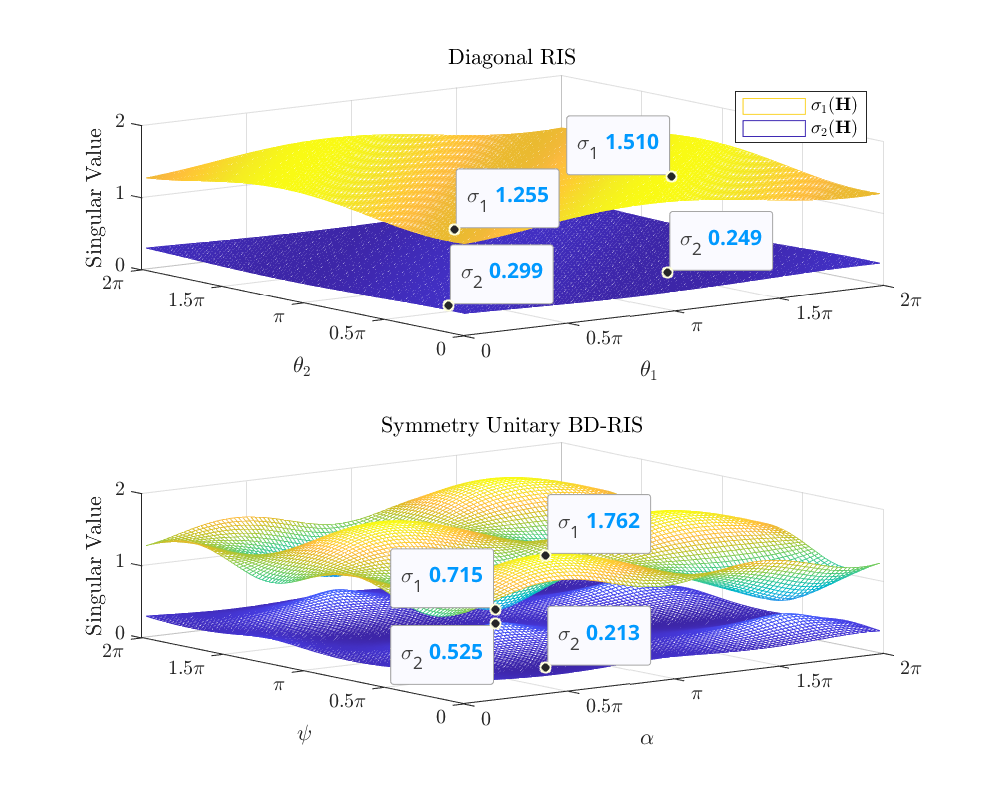
\includegraphics[width=\columnwidth]{assets/simulation/singular_trend.eps}
			\caption{$2 \times 2 \times 2$ (no direct) channel singular value shaping by diagonal and symmetry unitary \gls{ris}.}
			\label{fg:singular_trend}
		\end{figure}
		Fig.~\ref{fg:singular_trend} shows the channel singular values achieved by an exhaustive grid search over $(\theta_1, \theta_2)$ for diagonal \gls{ris} and $(\alpha, \psi)$ for symmetric unitary \gls{ris}.
		It is observed that both singular values can be manipulated up to $9\%$ using diagonal \gls{ris} and $42\%$ using symmetric \gls{bd}-\gls{ris}, despite both architectures have the same number of scattering elements and design parameters.
		A larger performance gap is expected when asymmetric \gls{bd}-\gls{ris} is available.
		This example shows \gls{bd}-\gls{ris} can provide a wider dynamic range of channel singular values and motivates further studies on channel shaping.
	\end{subsection}

	\begin{subsection}{Pareto Frontier Characterization}
		We then characterize the Pareto frontier of channel singular values by maximizing their weighted sum
		\begin{maxi!}
			{\scriptstyle{\mathbf{\Theta}}}{\sum_n \rho_n \sigma_n(\mathbf{H})}{\label{op:pareto}}{\label{ob:pareto}}
			\addConstraint{\mathbf{\Theta}_g^\mathsf{H} \mathbf{\Theta}_g=\mathbf{I},}{\quad \forall g,}{\label{co:pareto_unitary}}
		\end{maxi!}
		where $n \in \{1,\ldots,N \triangleq \min(N_\mathrm{T}, N_\mathrm{R})\}$ and $\rho_n$ is the weight of the $n$-th singular value that can be positive, zero, or negative.
		Varying $\{\rho_n\}$ unveils the entire achievable singular value region.
		Thus, the Pareto frontier problem~\eqref{op:pareto} generalizes most relevant metrics and provides a powerful shaping framework.
		The objective \eqref{ob:pareto} is smooth in $\mathbf{\Theta}$ and the feasible domain \eqref{co:pareto_unitary} for group $g$ corresponds to the Stiefel manifold.
		Next, we zoom out to general smooth maximization problems of asymmetric \gls{bd}-\gls{ris}.

		Inspired by \cite{Abrudan2008,Abrudan2009}, we propose a block-wise \gls{rcg} algorithm along the geodesics on the Lie group of unitary matrices $\mathbb{U}^{L \times L}$.
		It leverages the fact that unitary matrices are closed under multiplication.
		At iteration $r$, the gradient is computed in the Euclidean space and translated to the Riemannian manifold \cite{Absil2009}
		\begin{gather}
			\nabla_{\mathrm{E},g}^{(r)} = \frac{\partial f(\mathbf{\Theta}_g^{(r)})}{\partial \mathbf{\Theta}_g^*},\label{eq:gradient_euclidean}\\
			\nabla_{\mathrm{R},g}^{(r)} = \nabla_{\mathrm{E},g}^{(r)} {\mathbf{\Theta}_g^{(r)}}^\mathsf{H} - \mathbf{\Theta}_g^{(r)} {\nabla_{\mathrm{E},g}^{(r)}}^\mathsf{H}.\label{eq:gradient_riemannian}
		\end{gather}
		The Polak-Ribierre parameter \cite{Polak1969} is approximated as \cite{Abrudan2009}
		\begin{equation}
			\gamma_g^{(r)} = \frac{\mathrm{tr}\bigl((\nabla_{\mathrm{R},g}^{(r)} - \nabla_{\mathrm{R},g}^{(r-1)}) {\nabla_{\mathrm{R},g}^{(r)}}^\mathsf{H}\bigr)}{\mathrm{tr}\bigl(\nabla_{\mathrm{R},g}^{(r-1)} {\nabla_{\mathrm{R},g}^{(r-1)}}^\mathsf{H}\bigr)},
			\label{eq:parameter_cg}
		\end{equation}
		and the conjugate direction is
		\begin{equation}
			\mathbf{D}_g^{(r)} = \nabla_{\mathrm{R},g}^{(r)} + \gamma_g^{(r)} \mathbf{D}_g^{(r-1)}.
			\label{eq:direction_cg}
		\end{equation}
		In the Stiefel manifold, the geodesic emanating from $\mathbf{\Theta}_g^{(r)}$ with velocity $\mathbf{D}_g^{(r)}$ and step size $\mu$ is described compactly by the exponential map \cite{Edelman1998}
		\begin{equation}
			\mathbf{G}_g^{(r)}(\mu) = \exp(\mu \mathbf{D}_g^{(r)}) \mathbf{\Theta}_g^{(r)}.
			\label{eq:geodesic}
		\end{equation}
		An appropriate $\mu^\star$ can be obtained by the Armijo rule \cite{Armijo1966}.\footnote{To double the step size, one only need to square the rotation matrix instead of recomputing the matrix exponential, i.e., $\exp(2 \mu \mathbf{D}_g^{(r)}) = \exp^2(\mu \mathbf{D}_g^{(r)})$.}
		Finally, the scattering matrix is updated along the geodesic as
		\begin{equation}
			\mathbf{\Theta}_g^{(r+1)} = \mathbf{G}_g^{(r)}(\mu^\star).
			\label{eq:update_geodesic}
		\end{equation}
		Algorithm~\ref{ag:rcg} summarizes the proposed block-wise geodesic \gls{rcg} method for smooth maximization problems of asymmetric \gls{bd}-\gls{ris}.
		Convergence to stationary points is guaranteed.

		\begin{remark}
			Compared with universal manifold optimization \cite{Absil2009,Pan2022d}, Algorithm~\ref{ag:rcg} inherits a trifold benefit from \cite{Abrudan2008,Abrudan2009}:
			\begin{enumerate}
				\item No retraction thanks to rotational update \eqref{eq:geodesic}, \eqref{eq:update_geodesic};
				\item Lower computational complexity per iteration;
				\item Faster convergence thanks to proper parameter space.
			\end{enumerate}
		\end{remark}

		\setalgorithmcaptionfont{\small}
		\begin{algorithm}[!t]
			\small
			\caption{Block-wise geodesic \gls{rcg} for asymmetric \gls{bd}-\gls{ris}}
			\label{ag:rcg}
			\begin{algorithmic}[1]
				\Require $f(\mathbf{\Theta})$, $G$
				\Ensure $\mathbf{\Theta}^\star$
				\Initialize {$r \gets 0$, $\mathbf{\Theta}^{(0)}$}
				\Repeat
					\For {$g \gets 1$ to $G$}
						\State $\nabla_{\mathrm{E},g}^{(r)} \gets$ \eqref{eq:gradient_euclidean} \label{ln:gradient_euclidean}
						\State $\nabla_{\mathrm{R},g}^{(r)} \gets$ \eqref{eq:gradient_riemannian}
						\State $\gamma_g^{(r)} \gets$ \eqref{eq:parameter_cg}
						\State $\mathbf{D}_g^{(r)} \gets$ \eqref{eq:direction_cg}
						\If {$\Re\bigl\{\mathrm{tr}({\mathbf{D}_g^{(r)}}^\mathsf{H} \nabla_{\mathrm{R},g}^{(r)})\bigr\} < 0$} \Comment{not an ascent direction}
							\State $\mathbf{D}_g^{(r)} \gets \nabla_{\mathrm{R},g}^{(r)}$
						\EndIf
						\State $\mu \gets 1$
						\State $\mathbf{G}_g^{(r)}(\mu) \gets$ \eqref{eq:geodesic}
						\While {$f\bigl(\mathbf{G}_g^{(r)}(2\mu)\bigr) - f(\mathbf{\Theta}_g^{(r)}) \ge \mu \cdot \mathrm{tr}(\mathbf{D}_g^{(r)} {\mathbf{D}_g^{(r)}}^\mathsf{H}) / 2$}
							\State $\mu \gets 2 \mu$
						\EndWhile
						\While {$f\bigl(\mathbf{G}_g^{(r)}(\mu)\bigr) - f(\mathbf{\Theta}_g^{(r)}) < \mu / 2 \cdot \mathrm{tr}(\mathbf{D}_g^{(r)} {\mathbf{D}_g^{(r)}}^\mathsf{H}) / 2$}
							\State $\mu \gets \mu / 2$
						\EndWhile
						\State $\mathbf{\Theta}_g^{(r+1)} \gets$ \eqref{eq:update_geodesic}
					\EndFor
					\State $r \gets r+1$
				\Until $\lvert f(\mathbf{\Theta}^{(r)}) - f(\mathbf{\Theta}^{(r-1)}) \rvert / f(\mathbf{\Theta}^{(r-1)}) \le \epsilon$
			\end{algorithmic}
		\end{algorithm}

		\begin{lemma}\label{lm:pareto_gradient}
			The Euclidean gradient of \eqref{ob:pareto} w.r.t. \gls{bd}-\gls{ris} group $g$ is
			\begin{equation}
				\frac{\partial \sum_n \rho_n \sigma_n(\mathbf{H})}{\partial \mathbf{\Theta}_g^*} = \mathbf{H}_{\mathrm{B},g}^\mathsf{H} \mathbf{U} \mathrm{diag}(\rho_1,\ldots,\rho_N) \mathbf{V}^\mathsf{H} \mathbf{H}_{\mathrm{F},g}^\mathsf{H},
				\label{eq:pareto_gradient}
			\end{equation}
			where $\mathbf{U}$ and $\mathbf{V}$ are the left and right singular matrices of $\mathbf{H}$, respectively.
		\end{lemma}
		\begin{proof}
			Please refer to Appendix~\ref{ap:pareto_gradient}.
		\end{proof}

		%  The Euclidean gradient of \gls{bd}-\gls{ris} group $g$ is computed as
		% where $\mathbf{U} \in \mathbb{C}^{N_\mathrm{R} \times N}$ and $\mathbf{V} \in \mathbb{C}^{N_\mathrm{T} \times N}$ are the left and right compact singular matrices of $\mathbf{H}$, respectively.
		Algorithm~\ref{ag:rcg} can thus be invoked for the Pareto singular value problem \eqref{op:pareto} where line \ref{ln:gradient_euclidean} uses \eqref{eq:pareto_gradient} explicitly.
		% \eqref{eq:pareto_gradient} is used in line \ref{ln:gradient_euclidean}.
	\end{subsection}

	\begin{subsection}{Some Analytical Bounds}\label{sc:bounds}
		We then discuss some analytical bounds related to channel singular values.
		\begin{proposition}[degree of freedom]\label{pp:dof}
			In point-to-point \gls{mimo}, \gls{bd}-\gls{ris} cannot achieve a higher \gls{dof} than diagonal \gls{ris}.
		\end{proposition}
		\begin{proof}
			Please refer to Appendix~\ref{ap:dof}.
		\end{proof}

		\begin{proposition}[rank-deficient channel]\label{pp:rank_deficient}
			% If the forward/backward channel is rank-$k$, then a \gls{bd}-\gls{ris} can at most enlarge the $n$-th ($n > k$) channel singular value to the $n-k$-th singular value of $\mathbf{T}$, or suppress the $n$-th ($n < N - k + 1$) channel singular value to the $n$-th singular value of $\mathbf{T}$.
			% If the forward/backward channel is rank-$k$, then a sufficiently large \gls{bd}-\gls{ris} can at most enlarge (resp. suppress) the first (resp. last) $k$ equivalent channel singular values without bounds.
			If the forward or backward channel is rank-$k$, then regardless of the \gls{ris} size and architecture, the $n$-th singular value of the equivalent channel is bounded by
			\begin{align}
				\sigma_n(\mathbf{H}) & \le \sigma_{n-k}(\mathbf{T}), && \text{if } n > k, \label{iq:sv_bound_enlarge}\\
				\sigma_n(\mathbf{H}) & \ge \sigma_n(\mathbf{T}), && \text{if } n < N - k + 1, \label{iq:sv_bound_suppress}
			\end{align}
			where
			% \begin{align}
			% 	\mathbf{T} \mathbf{T}^\mathsf{H} = \mathbf{H}_\mathrm{D} (\mathbf{I} - \mathbf{V}_\mathrm{F} \mathbf{V}_\mathrm{F}^\mathsf{H}) \mathbf{H}_\mathrm{D}^\mathsf{H}, & \text{if } \mathrm{rank}(\mathbf{H}_\mathrm{F}) = k, \\
			% 	\mathbf{T}^\mathsf{H} \mathbf{T} = \mathbf{H}_\mathrm{D}^\mathsf{H} (\mathbf{I} - \mathbf{U}_\mathrm{F} \mathbf{U}_\mathrm{F}^\mathsf{H}) \mathbf{H}_\mathrm{D}, & \text{if } \mathrm{rank}(\mathbf{H}_\mathrm{B}) = k.
			% \end{align}
			\begin{equation}
				\mathbf{T} \mathbf{T}^\mathsf{H} =
				\begin{cases}
					\mathbf{H}_\mathrm{D} (\mathbf{I} - \mathbf{V}_\mathrm{F} \mathbf{V}_\mathrm{F}^\mathsf{H}) \mathbf{H}_\mathrm{D}^\mathsf{H}, & \text{if } \mathrm{rank}(\mathbf{H}_\mathrm{F}) = k, \\
					\mathbf{H}_\mathrm{D}^\mathsf{H} (\mathbf{I} - \mathbf{U}_\mathrm{B} \mathbf{U}_\mathrm{B}^\mathsf{H}) \mathbf{H}_\mathrm{D}, & \text{if } \mathrm{rank}(\mathbf{H}_\mathrm{B}) = k,
				\end{cases}
				\label{eq:auxiliary_matrix}
			\end{equation}
			and $\mathbf{V}_\mathrm{F}$ and $\mathbf{U}_\mathrm{B}$ are the right and left compact singular matrices of $\mathbf{H}_\mathrm{F}$ and $\mathbf{H}_\mathrm{B}$, respectively.
			% where $\mathbf{T} \mathbf{T}^\mathsf{H} = \mathbf{H}_\mathrm{D} (\mathbf{I} - \mathbf{V}_\mathrm{F} \mathbf{V}_\mathrm{F}^\mathsf{H}) \mathbf{H}_\mathrm{D}$ if the forward channel is rank-$k$ and $\mathbf{T}^\mathsf{H} \mathbf{T} = \mathbf{H}_\mathrm{D} (\mathbf{I} - \mathbf{U}_\mathrm{F} \mathbf{U}_\mathrm{F}^\mathsf{H}) \mathbf{H}_\mathrm{D}$ if the backward channel is rank-$k$.
		\end{proposition}
		\begin{proof}
			Please refer to Appendix~\ref{ap:rank_deficient}.
		\end{proof}

		% \begin{corollary}[degree of freedom]
		% 	In point-to-point \gls{mimo} with or without direct link, \gls{bd}-\gls{ris} cannot provide a higher \gls{dof} than diagonal \gls{ris}.
		% \end{corollary}

		\begin{corollary}[extreme singular values\label{co:extreme}]
			With a sufficiently large \gls{ris}, the first $k$ channel singular values are unbounded above while the last $k$ channel singular values can be suppressed to zero.
			% For a rank-$k$ forward or backward channel with a sufficiently large \gls{ris}, the first $k$ singular values of the equivalent channel are unbounded above while the last $k$ singular values can be suppressed to zero.
			% If the forward or backward channel is rank-$k$ and the \gls{ris} is sufficiently large, then the first $k$ singular values of the equivalent channel are unbounded above while the last $k$ singular values can be suppressed to zero.
			% If the forward/backward channel is rank-$k$, then the first (resp. last) $k$ singular values of the equivalent channel are unbounded above (resp. below).
			% a sufficiently large \gls{ris} can at most enlarge (resp. suppress) the first (resp. last) $k$ singular values of the equivalent channel without bounds.
		\end{corollary}

		\begin{corollary}[\gls{los} channel\footnote{A similar result has been derived for diagonal \gls{ris} in \cite{Semmler2023}.}\label{co:los}]
			If the forward or backward channel is \gls{los}, then a \gls{ris} can at most enlarge (resp. suppress) the $n$-th ($n \ge 2$) channel singular value to the $(n-1)$-th (resp. $n$-th) singular value of $\mathbf{T}$, that is,
			\begin{equation}
				\sigma_1(\mathbf{H}) \ge \sigma_1(\mathbf{T}) \ge {\sigma_2(\mathbf{H})} \ge \ldots \ge \sigma_{N-1}(\mathbf{T}) \ge {\sigma_N(\mathbf{H})} \ge \sigma_N(\mathbf{T}).
				\label{iq:sv_bound_los}
			\end{equation}
		\end{corollary}

		In Section~\ref{sc:simulation}, we will show by simulation that a finite-size \gls{bd}-\gls{ris} can approach those bounds better than diagonal \gls{ris}.

		\begin{proposition}[fully-connected \gls{ris} without direct link]\label{pp:fully_connected}
			% If the \gls{bd}-\gls{ris} is fully-connected and the direct link is absent, then the singular value bounds on $\mathbf{H}$ are equivalent to the singular value bounds on $\mathbf{BF}$, where $\mathbf{B}$ and $\mathbf{F}$ are arbitrary matrices with the same singular values as $\mathbf{H}_\mathrm{B}$ and $\mathbf{H}_\mathrm{F}$, respectively,
			If the \gls{bd}-\gls{ris} is fully-connected and the direct link is absent, then the channel singular values can be manipulated up to
			% If the \gls{bd}-\gls{ris} is fully-connected and the direct link is absent, then the bounds on the channel singular values are equivalent to the singular values of the equivalent channel, that is,
			% only bounds that apply here are those that apply to the singular values of
			\begin{equation}
				\mathrm{sv}(\mathbf{H}) = \mathrm{sv}(\mathbf{BF}),
			\end{equation}
			where $\mathbf{B}$ and $\mathbf{F}$ are arbitrary matrices with the same singular values as $\mathbf{H}_\mathrm{B}$ and $\mathbf{H}_\mathrm{F}$, respectively,
			% Our focus thus shifts to how the singular values of matrix product are bounded by the singular values of its individual factors.
		\end{proposition}

		\begin{proof}
			Please refer to Appendix~\ref{ap:fully_connected}.
		\end{proof}

		The problem now becomes how the singular values of matrix product are bounded by the singular values of its individual factors.
		Let $N' = \max(N_\mathrm{T},N_\mathrm{S},N_\mathrm{R})$ and $\sigma_n(\mathbf{H})=\sigma_n(\mathbf{H}_\mathrm{F})=\sigma_n(\mathbf{H}_\mathrm{B})=0$ for $N < n \le N'$.
		We have the following corollaries.

		\begin{corollary}[generic singular value bounds \cite{Fulton2000}]
			\begin{equation}
				\prod_{k \in {K}} \sigma_k(\mathbf{H}) \le \prod_{i \in {I}} \sigma_i(\mathbf{H}_\mathrm{B}) \prod_{j \in {J}} \sigma_j(\mathbf{H}_\mathrm{F}),
				\label{iq:sv_bound_fc}
			\end{equation}
			for all admissible triples $(I, J, K) \in T_r^{N'}$ with $r < N'$, where
			\begin{equation*}
				\begin{gathered}
					% T_r^{N'} \triangleq \Bigl\{(I, J, K) \in U_r^{N'} \mid \text{for all } p < r \text{ and all } (F, G, H) \text{ in } T_p^r,\\
					% \sum_{f \in F} i_f + \sum_{g \in G} j_g \le \sum_{h \in H} k_h + p(p+1)/2 \Bigr\},
					T_r^{N'} \triangleq \Bigl\{(I, J, K) \in U_r^{N'} \mid \forall p < r, (F, G, H) \in T_p^r,\\
					\sum_{f \in F} i_f + \sum_{g \in G} j_g \le \sum_{h \in H} k_h + p(p+1)/2 \Bigr\},
				\end{gathered}
			\end{equation*}
			\begin{equation*}
				U_r^{N'} \triangleq \Bigl\{(I, J, K) \mid \sum_{i \in I} i + \sum_{j \in J} j = \sum_{k \in K} k + r(r+1)/2\Bigr\}.
			\end{equation*}
		\end{corollary}

		\begin{corollary}[upper bound on the largest singular value]
			\begin{equation}
				\sigma_1(\mathbf{H}) \le \sigma_1(\mathbf{H}_\mathrm{B}) \sigma_1(\mathbf{H}_\mathrm{F}).
			\end{equation}
		\end{corollary}

		% \begin{corollary}[lower bound on the smallest singular value]
		% 	\begin{equation}
		% 		\sigma_{N'}(\mathbf{H}) \ge \sigma_{N'}(\mathbf{H}_\mathrm{B}) \sigma_{N'}(\mathbf{H}_\mathrm{F}).
		% 	\end{equation}
		% \end{corollary}

		\begin{corollary}[upper bound on the product of first $k$ singular values]
			\begin{equation}
				\prod_{n=1}^k \sigma_n(\mathbf{H}) \le \prod_{n=1}^k \sigma_n(\mathbf{H}_\mathrm{B}) \prod_{n=1}^k \sigma_n(\mathbf{H}_\mathrm{F}).
			\end{equation}
		\end{corollary}

		% \begin{corollary}[lower bound on the product of last $k$ singular values]
		% 	\begin{equation}
		% 		\prod_{n=N'}^{N'-k+1} \sigma_n(\mathbf{H}) \ge \prod_{n=N'}^{N'-k+1} \sigma_n(\mathbf{H}_\mathrm{B}) \prod_{n=N'}^{N'-k+1} \sigma_n(\mathbf{H}_\mathrm{F}).
		% 	\end{equation}
		% \end{corollary}

		\begin{corollary}[upper bound on the sum of first $k$ singular values to the power of $p$\label{co:sum_power}]
			\begin{equation}
				\sum_{n=1}^k \sigma_n^p(\mathbf{H}) \le \sum_{n=1}^k \sigma_n^p(\mathbf{H}_\mathrm{B}) \sigma_n^p(\mathbf{H}_\mathrm{F}), \quad p > 0.
				\label{iq:sv_bound_fc_power}
			\end{equation}
			When $k = N'$ and $p = 2$, \eqref{iq:sv_bound_fc_power} suggests the channel power is upper bounded by the sum of (sorted) element-wise power product of backward and forward subchannels.
		\end{corollary}

		\begin{remark}
			From \eqref{eq:scattering_fc} and \eqref{eq:channel_equivalent_fc} in the proof of Proposition \ref{pp:fully_connected}, we notice that \eqref{iq:sv_bound_fc}--\eqref{iq:sv_bound_fc_power} are simultaneously tight when
			% Interestingly, \eqref{iq:sv_bound_fc}--\eqref{iq:sv_bound_fc_power} are simultaneously tight when
			\begin{equation}
				\mathbf{\Theta} = \mathbf{V}_\mathrm{B} \mathbf{U}_\mathrm{F}^\mathsf{H}.
				\label{eq:scattering_fc_tight}
			\end{equation}
			An interpretation is that the off-diagonal entries can enhance the capabilities of
			\begin{itemize}
				\item subspace alignment: $\mathbf{V}_\mathrm{B}$ and $\mathbf{U}_\mathrm{F}^\mathsf{H}$ in \eqref{eq:scattering_fc} fully align the subspaces of $\mathbf{H}_\mathrm{B}$ and $\mathbf{H}_\mathrm{F}$ by rotation;
				\item subchannel rearrangement: $\mathbf{X} = \mathbf{I}$ in \eqref{eq:channel_equivalent_fc} pairs the subchannels of $\mathbf{H}_\mathrm{B}$ and $\mathbf{H}_\mathrm{F}$ from strongest to weakest, which attains the maximal in rearrangement inequality.
			\end{itemize}
		\end{remark}

		Tight bounds are inapplicable when a \gls{mimo} direct link is present, as the \gls{ris} needs to balance the direct-indirect (additive) and backward-forward (multiplicative) subspace alignments.
		Such a balance often involves optimization approaches and another example will be discussed in Section~\ref{sc:low_complexity}.
	\end{subsection}

\end{section}

\begin{section}{Achievable Rate Maximization}\label{sc:rate}
	The \gls{mimo} achievable rate maximization problem is formulated w.r.t. joint active and passive beamforming
	\begin{maxi!}
		{\scriptstyle{\mathbf{W},\mathbf{\Theta}}}{R = \log \det \biggl(\mathbf{I} + \frac{\mathbf{W}^\mathsf{H}\mathbf{H}^\mathsf{H}\mathbf{H}\mathbf{W}}{\eta}\biggr)}{\label{op:rate}}{\label{ob:rate}}
		\addConstraint{\lVert \mathbf{W} \rVert _\mathrm{F}^2 \le P}{}{}
		\addConstraint{\mathbf{\Theta}_g^\mathsf{H} \mathbf{\Theta}_g=\mathbf{I}, \quad \forall g,}{}{}
	\end{maxi!}
	where $\mathbf{W}$ is the transmit precoder, $R$ is the achievable rate, $\eta$ is the noise power, and $P$ is the transmit power budget.
	Two methods are proposed below to solve problem \eqref{op:rate}.

	\begin{subsection}{Alternating Optimization}
		Consider an \gls{ao} approach that updates $\mathbf{\Theta}$ and $\mathbf{W}$ iteratively.
		For a given $\mathbf{W}$, the passive beamforming subproblem is
		\begin{maxi!}
			{\scriptstyle{\mathbf{\Theta}}}{\log \det \biggl(\mathbf{I} + \frac{\mathbf{H} \mathbf{Q} \mathbf{H}^\mathsf{H}}{\eta}\biggr)}{\label{op:rate_passive}}{\label{ob:rate_passive}}
			\addConstraint{\mathbf{\Theta}_g^\mathsf{H} \mathbf{\Theta}_g=\mathbf{I}, \quad \forall g,}{}{}
		\end{maxi!}
		where $\mathbf{Q} \triangleq \mathbf{W} \mathbf{W}^\mathsf{H}$ is the transmit covariance matrix.
		\begin{lemma}\label{lm:rate_gradient}
			The Euclidean gradient of \eqref{ob:rate_passive} w.r.t. \gls{bd}-\gls{ris} block $g$ is
			\begin{equation}
				\frac{\partial R}{\partial \mathbf{\Theta}_g^*} = \frac{1}{\eta} \mathbf{H}_{\mathrm{B},g}^\mathsf{H} \biggl(\mathbf{I} + \frac{\mathbf{H}\mathbf{Q}\mathbf{H}^\mathsf{H}}{\eta}\biggr)^{-1} \mathbf{H} \mathbf{Q} \mathbf{H}_{\mathrm{F},g}^\mathsf{H}.
				\label{eq:rate_gradient}
			\end{equation}
		\end{lemma}

		\begin{proof}
			Please refer to Appendix~\ref{ap:rate_gradient}.
		\end{proof}
		Algorithm \ref{ag:rcg} is then invoked to solve problem \eqref{op:rate} where line \ref{ln:gradient_euclidean} uses \eqref{eq:rate_gradient} explicitly.
		Since \eqref{ob:rate_passive} is a concave function of $\mathbf{\Theta}$, convergence to local-optimal points is guaranteed.
		On the other hand, the global optimal transmit precoder for a fixed $\mathbf{\Theta}$ is given by the eigenmode transmission \cite{Clerckx2013}
		\begin{equation}
			\mathbf{W}^\star = \mathbf{V} {\mathbf{S}^\star}^{1/2},
			\label{eq:precoder_eigenmode}
		\end{equation}
		where $\mathbf{V}$ is the right channel singular matrix and $\mathbf{S}^\star$ is the optimal water-filling power allocation matrix.
		The overall \gls{ao} algorithm converges to local-optimal points of problem \eqref{op:rate} since each subproblem is solved optimally and the objective is bounded above.
	\end{subsection}

	\begin{subsection}{Low-Complexity Solution}\label{sc:low_complexity}
		We then propose a low-complexity solution to problem \eqref{op:rate} based on channel shaping.
		The passive beamforming subproblem \eqref{op:rate_passive} involves transmit covariance matrix $\mathbf{Q}$ and thus requires iterative \gls{rcg} update.
		Instead, we decouple the joint \gls{ris}-transceiver design by recasting \eqref{op:rate_passive} as channel power maximization
		\begin{maxi!}
			{\scriptstyle{\mathbf{\Theta}}}{\lVert \mathbf{H}_\mathrm{D} + \mathbf{H}_\mathrm{B} \mathbf{\Theta} \mathbf{H}_\mathrm{F} \rVert _\mathrm{F}^2}{\label{op:power_passive}}{\label{ob:power_passive}}
			\addConstraint{\mathbf{\Theta}_g^\mathsf{H} \mathbf{\Theta}_g=\mathbf{I}, \quad \forall g.}{}{}
		\end{maxi!}
		% which only accounts for channel characteristics but has no trivial solution.
		\begin{remark}
			As mentioned in Section \ref{sc:bounds}, the key of solving \eqref{op:power_passive} is to balance the additive and multiplicative subspace alignments.
			Problem \eqref{op:power_passive} is very similar (in terms of maximizing the inner product of $\mathbf{H}_\mathrm{D}$ and $\mathbf{H}_\mathrm{B} \mathbf{\Theta} \mathbf{H}_\mathrm{F}$) to the weighted orthogonal Procrustes problem \cite{Gower2004}
			\begin{mini!}
				{\scriptstyle{\mathbf{\Theta}}}{\lVert \mathbf{H}_\mathrm{D} - \mathbf{H}_\mathrm{B} \mathbf{\Theta} \mathbf{H}_\mathrm{F} \rVert _\mathrm{F}^2}{\label{op:weighted_orthogonal_procrustes}}{}
				\addConstraint{\mathbf{\Theta}^\mathsf{H} \mathbf{\Theta}=\mathbf{I},}{}{}
			\end{mini!}
			which has no trivial solution.
			One lossy transformation, by moving $\mathbf{\Theta}$ to one side \cite{Bell2003}, formulates standard orthogonal Procrustes problems
			\begin{mini!}
				{\scriptstyle{\mathbf{\Theta}}}{\lVert \mathbf{H}_\mathrm{B}^\dagger \mathbf{H}_\mathrm{D} - \mathbf{\Theta} \mathbf{H}_\mathrm{F} \rVert _\mathrm{F}^2 \text{ or } \lVert \mathbf{H}_\mathrm{D} \mathbf{H}_\mathrm{F}^\dagger - \mathbf{H}_\mathrm{B} \mathbf{\Theta} \rVert _\mathrm{F}^2}{\label{op:standard_orthogonal_procrustes}}{}
				\addConstraint{\mathbf{\Theta}^\mathsf{H} \mathbf{\Theta}=\mathbf{I},}{}{}
			\end{mini!}
			which has global optimal solutions $\mathbf{\Theta}^\star = \mathbf{U} \mathbf{V}^\mathsf{H}$ where $\mathbf{U}$ and $\mathbf{V}$ are the left and right singular matrices of $\mathbf{H}_\mathrm{B}^\dagger \mathbf{H}_\mathrm{D} \mathbf{H}_\mathrm{F}^\mathsf{H}$ or $\mathbf{H}_\mathrm{B}^\mathsf{H} \mathbf{H}_\mathrm{D} \mathbf{H}_\mathrm{F}^\dagger$ \cite{Golub2013}.
			This naive solution will be compared with the one proposed below.
		\end{remark}

		Inspired by \cite{Nie2017}, we successively approximate the quadratic objective \eqref{ob:power_passive} by local Taylor expansions and solve each iteration in closed form.

		\begin{proposition}\label{pp:power}
			Starting from any $\mathbf{\Theta}^{(0)} \in \mathbb{U}^{N_\mathrm{S} \times N_\mathrm{S}}$, the sequence
			\begin{equation}
				\mathbf{\Theta}_g^{(r+1)} = \mathbf{U}_g^{(r)} \mathbf{V}_g^{(r)}, \quad \forall g
				\label{eq:scattering_power}
			\end{equation}
			converges to a stationary point of \eqref{op:power_passive}, where $\mathbf{U}_g^{(r)}$ and $\mathbf{V}_g^{(r)}$ are the left and right compact singular matrix of
			\begin{equation}
				\mathbf{M}_g^{(r)} = \mathbf{H}_{\mathrm{B},g}^\mathsf{H} \Bigl(\mathbf{H}_\mathrm{D} + \mathbf{H}_\mathrm{B} \mathrm{diag}\bigl(\mathbf{\Theta}_{[1:g-1]}^{(r+1)},\mathbf{\Theta}_{[g:G]}^{(r)}\bigr) \mathbf{H}_\mathrm{F}\Bigr) \mathbf{H}_{\mathrm{F},g}^\mathsf{H}
				\label{eq:auxiliary_matrix_power}
			\end{equation}
		\end{proposition}

		\begin{proof}
			Please refer to Appendix~\ref{ap:power}.
		\end{proof}
		Once the channel shaping problem \eqref{op:power_passive} is solved, the transmit precoder can be obtained by \eqref{eq:precoder_eigenmode}.
		This two-stage approach decouples both blocks and is computationally efficient.
	\end{subsection}

	% \begin{figure}[!t]
	% 	\centering
	% 	\subfloat[\gls{ris} Elements, $N^\mathrm{T} = 8$\label{fg:pc_rate_sx}]{
	% 		\resizebox{0.48\columnwidth}{!}{
	% 			% This file was created by matlab2tikz.
%
%The latest updates can be retrieved from
%  http://www.mathworks.com/matlabcentral/fileexchange/22022-matlab2tikz-matlab2tikz
%where you can also make suggestions and rate matlab2tikz.
%
\definecolor{mycolor1}{rgb}{0.00000,0.44706,0.74118}%
\definecolor{mycolor2}{rgb}{0.85098,0.32549,0.09804}%
%
\begin{tikzpicture}

\begin{axis}[%
width=7.607cm,
height=6cm,
at={(0cm,0cm)},
scale only axis,
xmin=-10,
xmax=30,
xlabel style={font=\color{white!15!black}},
xlabel={Direct SNR [dB]},
ymin=0,
ymax=60,
ylabel style={font=\color{white!15!black}},
ylabel={Achievable Rate [bit/s/Hz]},
axis background/.style={fill=white},
xmajorgrids,
ymajorgrids,
legend style={at={(0.03,0.97)}, anchor=north west, legend cell align=left, align=left, draw=white!15!black}
]
\addplot [color=black, line width=2.0pt]
  table[row sep=crcr]{%
-10	1.36546104868107\\
0	5.88537073819504\\
10	15.6479397698849\\
20	28.3545786367547\\
30	41.5803303056336\\
};
\addlegendentry{$N_s = 0$}

\addplot [color=mycolor1, line width=2.0pt, mark=o, mark options={solid, mycolor1}]
  table[row sep=crcr]{%
-10	1.58237983975058\\
0	6.50387837535644\\
10	16.8570947901563\\
20	29.7509492256546\\
30	42.9979138713491\\
};
\addlegendentry{$(N_s, L) = (32, 1)$}

\addplot [color=mycolor1, dashed, line width=2.0pt, mark=o, mark options={solid, mycolor1}]
  table[row sep=crcr]{%
-10	1.66761899571824\\
0	6.86015391678907\\
10	17.558641485772\\
20	30.5085404030891\\
30	43.7595094694537\\
};
\addlegendentry{$(N_s, L) = (32, 4)$}

\addplot [color=mycolor1, dotted, line width=2.0pt, mark=o, mark options={solid, mycolor1}]
  table[row sep=crcr]{%
-10	1.70198084326635\\
0	7.07761307084566\\
10	18.0075672651913\\
20	30.9873193827021\\
30	44.2430615141333\\
};
\addlegendentry{$(N_s, L) = (32, 32)$}

\addplot [color=mycolor2, line width=2.0pt, mark=+, mark options={solid, mycolor2}]
  table[row sep=crcr]{%
-10	3.12887098831763\\
0	10.3906425812424\\
10	22.8418905336598\\
20	36.0211679842767\\
30	49.2965127222328\\
};
\addlegendentry{$(N_s, L) = (256, 1)$}

\addplot [color=mycolor2, dashed, line width=2.0pt, mark=+, mark options={solid, mycolor2}]
  table[row sep=crcr]{%
-10	3.89754922195652\\
0	13.0217363041026\\
10	26.051145903396\\
20	39.2688611043277\\
30	52.5427674698922\\
};
\addlegendentry{$(N_s, L) = (256, 4)$}

\addplot [color=mycolor2, dotted, line width=2.0pt, mark=+, mark options={solid, mycolor2}]
  table[row sep=crcr]{%
-10	4.21684458588047\\
0	14.1060943448495\\
10	27.9675046836052\\
20	41.2102781687149\\
30	54.4927123740025\\
};
\addlegendentry{$(N_s, L) = (256, 256)$}

\end{axis}
\end{tikzpicture}%
	% 		}
	% 	}
	% 	\subfloat[Transmit Antenna, $N^\mathrm{S} = 256$\label{fg:pc_rate_tx}]{
	% 		\resizebox{0.48\columnwidth}{!}{
	% 			% This file was created by matlab2tikz.
%
%The latest updates can be retrieved from
%  http://www.mathworks.com/matlabcentral/fileexchange/22022-matlab2tikz-matlab2tikz
%where you can also make suggestions and rate matlab2tikz.
%
\definecolor{mycolor1}{rgb}{0.00000,0.44706,0.74118}%
\definecolor{mycolor2}{rgb}{0.85098,0.32549,0.09804}%
\definecolor{mycolor3}{rgb}{0.92941,0.69412,0.12549}%
%
\begin{tikzpicture}

\begin{axis}[%
width=9.509cm,
height=7.5cm,
at={(0cm,0cm)},
scale only axis,
xmin=-10,
xmax=30,
% xlabel style={font=\color{white!15!black}},
xlabel={Direct SNR [dB]},
ymin=0,
ymax=60,
% ylabel style={font=\color{white!15!black}},
ylabel={Achievable Rate [bit/s/Hz]},
axis background/.style={fill=white},
xmajorgrids,
ymajorgrids,
legend style={at={(0.03,0.97)}, anchor=north west, legend cell align=left, align=left, draw=white!15!black}
]
\addplot [color=mycolor1, line width=2.0pt, mark=o, mark options={solid, mycolor1}]
  table[row sep=crcr]{%
-10	1.82485438191362\\
0	4.7222906563119\\
10	7.99393509732638\\
20	11.3107371667968\\
30	14.6321519880831\\
};
\addlegendentry{$(N^\mathrm{T}, L) = (1, 1)$}

\addplot [color=mycolor1, dashed, line width=2.0pt, mark=o, mark options={solid, mycolor1}]
  table[row sep=crcr]{%
-10	2.24659926648999\\
0	5.26330445507328\\
10	8.55078517680736\\
20	11.8692222057207\\
30	15.1908007320325\\
};
\addlegendentry{$(N^\mathrm{T}, L) = (1, 256)$}

\addplot [color=mycolor2, line width=2.0pt, mark=+, mark options={solid, mycolor2}]
  table[row sep=crcr]{%
-10	2.49039510987196\\
0	8.06192104582032\\
10	17.6588170852107\\
20	32.7099587384036\\
30	45.9789160838128\\
};
\addlegendentry{$(N^\mathrm{T}, L) = (4, 1)$}

\addplot [color=mycolor2, dashed, line width=2.0pt, mark=+, mark options={solid, mycolor2}]
  table[row sep=crcr]{%
-10	3.77849180447307\\
0	13.3359194935281\\
10	26.0483499099173\\
20	39.2753832167713\\
30	52.5569826592083\\
};
\addlegendentry{$(N^\mathrm{T}, L) = (4, 256)$}

\addplot [color=mycolor3, line width=2.0pt, mark=square, mark options={solid, mycolor3}]
  table[row sep=crcr]{%
-10	3.8179809156775\\
0	12.9043718464691\\
10	25.5833268533688\\
20	38.8067308900334\\
30	52.0881220415066\\
};
\addlegendentry{$(N^\mathrm{T}, L) = (16, 1)$}

\addplot [color=mycolor3, dashed, line width=2.0pt, mark=square, mark options={solid, mycolor3}]
  table[row sep=crcr]{%
-10	5.83961863479039\\
0	16.7543020939844\\
10	29.7401886345762\\
20	42.9967723667009\\
30	56.2807797979848\\
};
\addlegendentry{$(N^\mathrm{T}, L) = (16, 256)$}

\end{axis}

\begin{axis}[%
width=12.27cm,
height=9.202cm,
at={(-1.595cm,-1.012cm)},
scale only axis,
xmin=0,
xmax=1,
ymin=0,
ymax=1,
axis line style={draw=none},
ticks=none,
axis x line*=bottom,
axis y line*=left
]
\end{axis}
\end{tikzpicture}%

	% 		}
	% 	}
	% 	\caption{Average achievable rate versus group size $L$. $N^\mathrm{R} = 4$, $(\Lambda^\mathrm{D}, \Lambda^\mathrm{F}, \Lambda^\mathrm{B}) = (65, 54, 46) \unit{dB}$.}
	% 	\label{fg:pc_rate}
	% \end{figure}

	% Fig.~\ref{fg:pc_rate_sx} illustrates how \gls{ris} configuration influences the \gls{mimo} \gls{pc} achievable rate.
	% To ensure a \qty{20}{bit/s/Hz} transmission, an \gls{snr} of \qty{13.5}{\dB} is required for a 8T4R system.
	% This value decreases to \qty{12.5}{\dB} (resp. \qty{8}{\dB}) when 32- (resp. 256-) element diagonal \gls{ris} is present.
	% If tetrads can be formed in \gls{bd}-\gls{ris}, the \gls{snr} can be reduced by another \qty{20}{\percent} (resp. \qty{44}{\percent}).
	% Further increase in $L$ yields a marginal gain and incurs $\mathcal{O}(L^2)$ connections.
	% We thus conclude dyadic or tetradic \gls{bd}-\gls{ris} usually strike a good balance between performance and complexity.



		% \begin{figure}[!t]
		% 	\centering
		% 	\resizebox{0.65\columnwidth}{!}{
		% 		\input{assets/simulation/power_sx.tex}
		% 	}
		% 	\caption{Average channel power versus \gls{ris} elements $N^\mathrm{S}$ and group size $L$. $(N^\mathrm{T}, N^\mathrm{R}) = (8, 4)$, $(\Lambda^\mathrm{D}, \Lambda^\mathrm{F}, \Lambda^\mathrm{B}) = (65, 54, 46) \unit{dB}$.}
		% 	\label{fg:power_sx}
		% \end{figure}

		% \begin{figure}[!t]
		% 	\centering
		% 	\subfloat[Without Direct Link\label{fg:pc_power_bond_nd}]{
		% 		\resizebox{0.48\columnwidth}{!}{
		% 			% This file was created by matlab2tikz.
%
%The latest updates can be retrieved from
%  http://www.mathworks.com/matlabcentral/fileexchange/22022-matlab2tikz-matlab2tikz
%where you can also make suggestions and rate matlab2tikz.
%
\definecolor{mycolor1}{rgb}{0.46667,0.67451,0.18824}%
\definecolor{mycolor2}{rgb}{0.92941,0.50588,0.59608}%
%
\begin{tikzpicture}

\begin{axis}[%
width=7.607cm,
height=6cm,
at={(0cm,0cm)},
scale only axis,
bar shift auto,
xmin=0,
xmax=6,
xtick={1,2,3,4,5},
xticklabels={{1},{4},{16},{64},{256}},
xlabel style={font=\color{white!15!black}},
xlabel={RIS Group Size},
ymin=0,
ymax=3.5e-05,
ylabel style={font=\color{white!15!black}},
ylabel={Channel Power [W]},
axis background/.style={fill=white},
xmajorgrids,
ymajorgrids,
legend style={at={(0.03,0.97)}, anchor=north west, legend cell align=left, align=left, draw=white!15!black}
]
\addplot[ybar, bar width=0.8, fill=mycolor1, draw=black, area legend] table[row sep=crcr] {%
1	7.67624350482862e-07\\
2	1.32530638063741e-06\\
3	3.06197930445936e-06\\
4	9.39519835024894e-06\\
5	3.02284526139409e-05\\
};
\addplot[forget plot, color=white!15!black] table[row sep=crcr] {%
0	0\\
6	0\\
};
\addlegendentry{Composite}

\addplot [color=black, line width=2.0pt]
  table[row sep=crcr]{%
-0.2	0\\
6.2	0\\
};
\addlegendentry{Direct}

\addplot [color=mycolor2, line width=2.0pt]
  table[row sep=crcr]{%
-0.2	3.04194803196479e-05\\
6.2	3.04194803196479e-05\\
};
\addlegendentry{Cascaded}

\end{axis}
\end{tikzpicture}%
		% 		}
		% 	}
		% 	\subfloat[With Direct Link\label{fg:pc_power_bond_hd}]{
		% 		\resizebox{0.48\columnwidth}{!}{
		% 			% This file was created by matlab2tikz.
%
%The latest updates can be retrieved from
%  http://www.mathworks.com/matlabcentral/fileexchange/22022-matlab2tikz-matlab2tikz
%where you can also make suggestions and rate matlab2tikz.
%
\definecolor{mycolor1}{rgb}{0.46667,0.67451,0.18824}%
\definecolor{mycolor2}{rgb}{0.92941,0.50588,0.59608}%
%
\begin{tikzpicture}

\begin{axis}[%
width=7.607cm,
height=6cm,
at={(0cm,0cm)},
scale only axis,
bar shift auto,
xmin=0,
xmax=6,
xtick={1,2,3,4,5},
xticklabels={{1},{4},{16},{64},{256}},
xlabel style={font=\color{white!15!black}},
xlabel={RIS Group Size},
ymin=0,
ymax=7e-05,
ylabel style={font=\color{white!15!black}},
ylabel={Channel Power [W]},
axis background/.style={fill=white},
xmajorgrids,
ymajorgrids,
legend style={at={(0.03,0.97)}, anchor=north west, legend cell align=left, align=left, draw=white!15!black}
]
\addplot[ybar, bar width=0.8, fill=mycolor1, draw=black, area legend] table[row sep=crcr] {%
1	2.83336295997331e-05\\
2	4.76924466169225e-05\\
3	6.08890936283682e-05\\
4	6.46004645413477e-05\\
5	6.64188484186803e-05\\
};
\addplot[forget plot, color=white!15!black] table[row sep=crcr] {%
0	0\\
6	0\\
};
\addlegendentry{Composite}

\addplot [color=black, line width=2.0pt]
  table[row sep=crcr]{%
-0.2	9.51300474293446e-06\\
6.2	9.51300474293446e-06\\
};
\addlegendentry{Direct}

\addplot [color=mycolor2, line width=2.0pt]
  table[row sep=crcr]{%
-0.2	3.07152044114707e-05\\
6.2	3.07152044114707e-05\\
};
\addlegendentry{Cascaded}

\end{axis}
\end{tikzpicture}%
		% 		}
		% 	}
		% 	\caption{Average channel power versus \gls{ris} group size $L$. $(N^\mathrm{T}, N^\mathrm{S}, N^\mathrm{R}) = (8, 256, 4)$, $(\Lambda^\mathrm{D}, \Lambda^\mathrm{F}, \Lambda^\mathrm{B}) = (65, 54, 46) \unit{dB}$.}
		% 	\label{fg:pc_power_bond}
		% \end{figure}
		% % Fig.~\ref{fg:power_sx} shows that, apart from numerous reflecting elements, a sufficiently large group size can help
		% % Fig.~\ref{fg:power_sx} shows that increasing the group size can improve the channel power especially for a large \gls{ris}.
		% Fig.~\ref{fg:power_sx} shows that, apart from adding reflecting elements $N^\mathrm{S}$, increasing the group size $L$ also improves the channel power.
		% % The behavior is more obvious for a large \gls{ris}.
		% This behavior is more pronounced for a large \gls{ris}.
		% For example, the gain of pairwise connection is \qty{2.8}{\percent} for $N^\mathrm{S} = 16$ and \qty{28}{\percent} for $N^\mathrm{S} = 256$.
		% % \gls{bd}-\gls{ris} provides a higher channel power than conventional \gls{ris}.
		% % As $L$ increases from 1 to 2,
		% It implies that the channel shaping capability of \gls{bd}-\gls{ris} scales with group size $L$.

		% Fig.~\ref{fg:pc_power_bond_hd} and \ref{fg:pc_power_bond_nd} compare the average channel power without and with direct link.
		% % where the cascaded channel power available to passive \gls{ris} is $\lVert \mathbf{H}^\mathrm{B} \rVert _\mathrm{F}^2 \lVert \mathbf{H}^\mathrm{F} \rVert _\mathrm{F}^2$.
		% % where the cascaded channel power available to passive \gls{ris} is $\lVert \mathbf{H}^\mathrm{B} \rVert _\mathrm{F}^2 \lVert \mathbf{H}^\mathrm{F} \rVert _\mathrm{F}^2$.
		% % ``Cascaded'' means the maximum power of the cascaded channel, i.e., $\lVert \mathbf{H}^\mathrm{B} \rVert _\mathrm{F}^2 \lVert \mathbf{H}^\mathrm{F} \rVert _\mathrm{F}^2$.
		% % maximum power of the cascaded channel, i.e., $\lVert \mathbf{H}^\mathrm{B} \rVert _\mathrm{F}^2 \lVert \mathbf{H}^\mathrm{F} \rVert _\mathrm{F}^2$.
		% % ? ``Cascaded'' means the \emph{power product} of the forward and backward channels.
		% % ``Cascaded'' means the sum of element-wise product of first $N = \min(N^\mathrm{T}, N^\mathrm{S}, N^\mathrm{R})$ eigenvalues of the forward and backward channels.
		% ``Cascaded'' means the sum of element-wise product of first $N = \min(N^\mathrm{T}, N^\mathrm{S}, N^\mathrm{R})$ eigenvalues (i.e., element-wise power product) of the forward and backward channels.
		% We observe that diagonal \gls{ris} wastes substantial cascaded power and struggles to align the direct-indirect eigenspace.
		% When the direct link is absent, only \qty{2.6}{\percent} of available power is utilized by diagonal \gls{ris} while \qty{100}{\percent} power is recycled by fully-connected \gls{ris}.
		% When the direct link is present, the proposed \gls{bd}-\gls{ris} design can balance the direct-indirect and forward-backward eigenspace alignment for an optimal channel boost.
		% It is worth noting that, when $L$ is sufficiently large, the composite channel power surpasses the power sum of direct and cascaded channels, thanks to the constructive \emph{amplitude superposition} of direct and cascaded channels.
		% This again emphasizes the advantage of in-group connection of \gls{bd}-\gls{ris}.
		% % This is because the direct and indirect channels superpose
		% % the proposed \gls{bd}-\gls{ris} design can also be applied to conventional \gls{ris} to improve the channel power.
		% % When the direct link is present, a small $L$ cannot align the direct-indirect eigenspace.

		% % neither effectively utilizes the cascaded channel power, nor effectively align the direct-indirect eigenspace.
		% % We observe that conventional \gls{ris} neither effectively utilizes the cascaded channel power, nor effectively align the direct-indirect eigenspace.
		% % For conventional \gls{ris},
		% % align the direct-indirect eigenspace.
		% % When the direct link is present, a small $L$ can neither align the direct-indirect eigenspace nor the forward-backward eigenspace.
		% % For a relatively large $N^\mathrm{S}$, conventional \gls{ris} cannot
		% % neither the direct-indirect nor the forward-backward eigenspace can be effectively aligned with a small $L$.

		% % When the direct link is present, a small $L$ can neither preserve the
		% % neither align the direct-indirect eigenspace nor the forward-backward eigenspace.

		% % When the direct link is absent, a large $L$ can align the forward-backward eigenspace but cannot preserve the forward-backward power balance.

\end{section}

\begin{section}{Simulation Results}\label{sc:simulation}
	In this section, we provide numerical results to evaluate the proposed \gls{bd}-\gls{ris} designs.
	Consider a distance-dependent path loss model $\Lambda(d) = \Lambda_0 d^{-\gamma}$ where $\Lambda_0$ is the reference path loss at distance \qty{1}{m}, $d$ is the propagation distance, and $\gamma$ is the path loss exponent.
	The small-scale fading model is $\mathbf{H} = \sqrt{\kappa/(1+\kappa)} \mathbf{H}_\text{LoS} + \sqrt{1/(1+\kappa)} \mathbf{H}_\text{NLoS}$, where $\kappa$ is the Rician $K$-factor, $\mathbf{H}_\text{LoS}$ is the deterministic \gls{los} component, and $\mathbf{H}_\text{NLoS} \sim \mathcal{CN}(\mathbf{0}, \mathbf{I})$ is the Rayleigh component.
	We set $\Lambda_0=\qty{-30}{dB}$, $d_\mathrm{D}=\qty{14.7}{m}$, $d_\mathrm{F}=\qty{10}{m}$, $d_\mathrm{B}=\qty{6.3}{m}$, $\gamma_\mathrm{D}=3$, $\gamma_\mathrm{F}=2.4$ and $\gamma_\mathrm{B}=2$ for reference, which corresponds to a typical indoor environment with $\Lambda_\mathrm{D}=\qty{-65}{dB}$, $\Lambda_\mathrm{F}=\qty{-54}{dB}$, $\Lambda_\mathrm{B}=\qty{-46}{dB}$.
	The indirect path via \gls{ris} is thus \qty{35}{\dB} weaker than the direct path.
	$\kappa \to \infty$ is assumed for all channels unless otherwise specified.

	\begin{subsection}{Channel Singular Values Redistribution}
		\begin{subsubsection}{Pareto Frontier}
			\begin{figure}[!t]
				\centering
				\subfloat[$2 \times 32 \times 2$ (no direct)\label{fg:singular_pareto_sx32_nd}]{
					\resizebox{0.48\columnwidth}{!}{
						% This file was created by matlab2tikz.
%
%The latest updates can be retrieved from
%  http://www.mathworks.com/matlabcentral/fileexchange/22022-matlab2tikz-matlab2tikz
%where you can also make suggestions and rate matlab2tikz.
%
\definecolor{mycolor1}{rgb}{0.00000,0.44706,0.74118}%
\definecolor{mycolor2}{rgb}{0.85098,0.32549,0.09804}%
\definecolor{mycolor3}{rgb}{0.92941,0.69412,0.12549}%
\definecolor{mycolor4}{rgb}{0.49412,0.18431,0.55686}%
%
\begin{tikzpicture}

\begin{axis}[%
width=7.607cm,
height=6cm,
at={(0cm,0cm)},
scale only axis,
xmin=0,
xmax=0.00038965048998045,
xlabel style={font=\color{white!15!black}},
xlabel={$\sigma_1$},
ymin=0,
ymax=0.000304493100518335,
ylabel style={font=\color{white!15!black}},
ylabel={$\sigma_2$},
axis background/.style={fill=white},
xmajorgrids,
ymajorgrids,
legend style={at={(0.03,0.97)}, anchor=north west, legend cell align=left, align=left, draw=white!15!black},
every axis plot/.append style={line width=1.5pt}
]
\addplot[only marks, mark=triangle, mark options={}, mark size=2.3570pt, draw=black] table[row sep=crcr]{%
x	y\\
0	0\\
};
\addlegendentry{Direct}

\addplot [color=mycolor1, line width=2.0pt, mark=o, mark options={solid, mycolor1}]
  table[row sep=crcr]{%
0.000267895667198245	0.000171134879393267\\
0.000265726380728974	0.000173150928555956\\
0.000263620365603918	0.000175013140296501\\
0.000261445144530834	0.000176843202895948\\
0.000259164875117885	0.000178667936743009\\
0.000256772775708205	0.000180487719376887\\
0.000254278514486235	0.000182290392662069\\
0.000251704002269913	0.000184056601213238\\
0.000249073506157511	0.000185767894974696\\
0.000246400740748153	0.000187414817948743\\
0.000243687718680905	0.000188995994660418\\
0.000240928492221004	0.000190514582140261\\
0.000238098477127779	0.000191982763893684\\
0.000235165035954025	0.000193414254436945\\
0.000232089995279799	0.000194822374050852\\
0.000228824413086908	0.000196221753795029\\
0.000225316977451163	0.000197623817299328\\
0.000221535346161309	0.000199028850294541\\
0.000203259528520131	0.000203259526698551\\
0.000199827287451323	0.000199827287443645\\
0.000198123535486915	0.000198123535486911\\
0.000180148810088901	0.0001801488100889\\
8.42468741466946e-21	6.05571416226906e-21\\
6.19979890484365e-21	3.35030862543257e-21\\
6.60756407329265e-21	1.28456637898193e-21\\
7.66177135693828e-21	3.92046971006709e-22\\
0.000180096069830613	1.08306169491646e-20\\
0.000191831039008028	1.66189243361953e-20\\
0.000264113777998769	7.79621614858511e-20\\
0.000279564446825807	4.05296860635826e-19\\
0.000280589608744265	1.14924619753218e-18\\
0.000281565424666408	3.19287626893919e-17\\
0.000294887428789775	6.22978162678605e-16\\
0.000298297210243084	1.4033135819947e-15\\
0.000309415141512222	5.02384211049284e-15\\
0.000312286791270632	6.622168556894e-15\\
0.000313941579001134	1.5519784325904e-11\\
0.000315080469539148	2.60442929195929e-06\\
0.000316650462662155	6.20803322481037e-06\\
0.000317953658131026	1.0637150181653e-05\\
0.000319531793152611	1.60801484565072e-05\\
0.000321145121813445	2.39596943662345e-05\\
0.000321463002882309	3.21072961439859e-05\\
0.000321532819016651	3.76429148560442e-05\\
0.000321472892430131	4.25828187614136e-05\\
0.000321300760117647	4.72640647983865e-05\\
0.000321020731972484	5.18237773689732e-05\\
0.000320633271897779	5.63231191746697e-05\\
0.000320137546722193	6.07926465706622e-05\\
0.00031953359137215	6.52391237196603e-05\\
0.000318820183056992	6.96729345667314e-05\\
0.000317997781544904	7.40900801825946e-05\\
0.000317066229794775	7.84903211168037e-05\\
0.000316024782888273	8.28755034268974e-05\\
0.000314867375461116	8.72664954039366e-05\\
0.000313584778992714	9.16888362417147e-05\\
0.000312161323906551	9.61814565544305e-05\\
0.000310588510709343	0.000100752805689686\\
0.000308886100168095	0.000105333037823099\\
0.000307099022755485	0.000109802296733328\\
0.000304874570657941	0.000114975407123897\\
0.000295523412404848	0.000136118926480847\\
0.000293796779560532	0.000139257271731018\\
0.000292107248523008	0.000142157036202118\\
0.000290431849142458	0.000144876663627326\\
0.000288754605499061	0.000147455239474912\\
0.000287064679129902	0.000149918781615647\\
0.000285354493393488	0.000152285164138566\\
0.000283619431704674	0.00015456587543467\\
0.000281858022889306	0.000156766916808042\\
0.000280067185001826	0.00015889544523825\\
0.000278240363912649	0.000160961566094741\\
0.000276367480760894	0.000162977751672099\\
0.000267895667198245	0.000171134879393267\\
};
\addlegendentry{$L = 1$}

\addplot [color=mycolor2, dashed, line width=2.0pt, mark=+, mark options={solid, mycolor2}]
  table[row sep=crcr]{%
0.000355739456151093	0.00023630212231011\\
0.000353983785016404	0.000238013710074763\\
0.000351859225447142	0.000239984970213792\\
0.000349054422291465	0.000242460729759867\\
0.000344270181551168	0.000246471602221089\\
0.000332985328589198	0.000255488751251254\\
0.000326266184355555	0.000260610115544627\\
0.000320562886323912	0.000264733162717323\\
0.000314325700971254	0.000269011913129879\\
0.000308560245761306	0.000272769530149513\\
0.000304688873039902	0.000275159663058865\\
0.000301895314065004	0.000276789729801272\\
0.000299616367457836	0.000278045082584301\\
0.000297629447604807	0.00027907656379607\\
0.000295820894328768	0.000279959625818801\\
0.000294119244751247	0.000280739245424517\\
0.000292480429716739	0.00028144185454148\\
0.000290869271980479	0.000282086202217012\\
0.000289258251330994	0.000282684955608739\\
0.000287439311775594	0.000283221155075434\\
0.000286111329523935	0.000283226241828683\\
0.000281749477516674	0.000281749467335335\\
0.000279440614092202	0.000279440611372918\\
0.000220457825755789	0.000220457825746552\\
0.000208068910616119	0.000208068910610979\\
0.000187946250277845	0.000187946250276701\\
0.000180148810088901	0.000180148810088901\\
6.5591718870255e-05	6.55917188702549e-05\\
4.20164701380515e-21	8.79388127033691e-22\\
6.32472477104445e-21	3.43356879819089e-22\\
0.000175524733181838	4.89153384024627e-21\\
0.000191831039008028	8.05014238109372e-21\\
0.000223156565739869	2.18554354445088e-20\\
0.000298795369668053	4.43259933963327e-19\\
0.000319836197632342	1.14449267159391e-17\\
0.000337395279306117	2.33052717459466e-17\\
0.000345669096124742	1.5235327945565e-16\\
0.000371901015970715	7.29825031398575e-16\\
0.000372437013168705	1.73328225712588e-13\\
0.000372486831885383	2.81023595538404e-05\\
0.000372471466593596	0.000201236641395997\\
0.000372426852724318	0.000202454117307786\\
0.000372354749362613	0.000203628518387191\\
0.000372256427569083	0.000204770528112299\\
0.000372133071603637	0.000205882935186015\\
0.000371985309281415	0.000206970833147438\\
0.000371813719503542	0.000208037182759402\\
0.00037161832382613	0.000209086468304937\\
0.00037139955457068	0.000210119666912738\\
0.00037115668565401	0.000211142180316026\\
0.000370889086656138	0.000212157232410383\\
0.000370596708144513	0.000213165221964369\\
0.000370278106444865	0.000214170692984417\\
0.000369931918553916	0.000215176768360127\\
0.000369557062102171	0.000216184995411197\\
0.000369151325283754	0.000217199302911258\\
0.000368713688516441	0.000218219947660847\\
0.000368241418310008	0.000219250752341472\\
0.000367731914734066	0.000220294367526888\\
0.000367183349266502	0.000221351363599926\\
0.000366591723007183	0.000222425941716797\\
0.000365955230149435	0.00022351770001446\\
0.000365268517707625	0.00022463180272036\\
0.000364529269287204	0.000225767731198768\\
0.000363731076897723	0.000226930750043674\\
0.00036286865154264	0.000228123468496278\\
0.000361936078587719	0.000229348684335404\\
0.000360923096272773	0.000230613841212628\\
0.000359816798832403	0.000231927997905375\\
0.000358602593712985	0.000233300381138745\\
0.000357257858194128	0.000234747077469494\\
0.000355739456151093	0.00023630212231011\\
};
\addlegendentry{$L = 4$}

\addplot [color=mycolor3, dotted, line width=2.0pt, mark=square, mark options={solid, mycolor3}]
  table[row sep=crcr]{%
0.000387644725001034	0.000252163649786122\\
0.000387494244577878	0.000252309874048033\\
0.000387321385451581	0.00025246982456047\\
0.000387123619656507	0.00025264497436984\\
0.000354044414728323	0.000278788391537759\\
0.000324031566213212	0.00030181769538482\\
0.000323370970606122	0.000302322033286758\\
0.000322939503948698	0.000302634503158319\\
0.000322629710522514	0.000302847188929005\\
0.000322389738998535	0.0003030037313976\\
0.000322192012399091	0.000303125657570389\\
0.000322021223310372	0.000303225205191342\\
0.000321868058470525	0.000303309585408043\\
0.000321726332885747	0.00030338319606735\\
0.000321591838228086	0.000303448853401541\\
0.000321461357536437	0.000303508427690401\\
0.000321333801566517	0.000303563282339639\\
0.000321206511969601	0.000303614207600706\\
0.000321078376511536	0.00030366181921831\\
0.000320948398043425	0.00030370654144927\\
0.000320815486892904	0.000303748637788079\\
0.000320678813033656	0.000303788277927965\\
0.000309564989052386	0.000301409733854497\\
0.000288166772576663	0.000287746907546531\\
0.000279440619857278	0.000279440619671027\\
0.000220457825773397	0.000220457825766601\\
0.000193478737274631	0.000193478737273387\\
0.000187946250278386	0.00018794625027787\\
0.000180148810088901	0.000180148810088901\\
7.38779007531488e-05	7.38779007531487e-05\\
6.5591718870255e-05	6.55917188702549e-05\\
6.11855785437379e-21	3.45293064321707e-21\\
4.20164701380515e-21	8.79388127033691e-22\\
1.54145558743596e-20	4.5368881526408e-22\\
0.000121848054411894	4.00695794022811e-21\\
0.000191831039008028	8.05014238109372e-21\\
0.000298795369668053	1.54041673309025e-20\\
0.000319836197632354	2.36457288348854e-18\\
0.000333476889166338	1.75021877124016e-17\\
0.000335729299617477	4.56099183583301e-17\\
0.000337395279306272	8.16975720607573e-17\\
0.000345669096125748	4.1981459702903e-16\\
0.000346031641514439	4.39830021468541e-15\\
0.000387914582890843	1.13358549119329e-12\\
0.000388584823891499	8.0163235518879e-12\\
0.000389055459349451	2.17977036180119e-08\\
0.000389129203196301	2.36054120455867e-05\\
0.000389090206430443	0.000249310691234572\\
0.000389037671865594	0.00024972476835498\\
0.000388990920465773	0.000249934686797231\\
0.000388964382651109	0.000250035016505946\\
0.000388935788614941	0.000250134077714785\\
0.000388905063299093	0.000250231182320069\\
0.000388872172163426	0.000250326693388387\\
0.000388837071247733	0.00025042106587312\\
0.000388799688709563	0.000250514636529308\\
0.000388759882275995	0.000250607325760949\\
0.00038871754306719	0.000250699736848645\\
0.000388672525582172	0.000250792084880618\\
0.000388624572418996	0.000250884495860529\\
0.000388573499339921	0.000250977447103048\\
0.000388518934001622	0.000251071035900666\\
0.000388460497180009	0.000251165596815782\\
0.000388397897277804	0.000251262019216711\\
0.000388330323709399	0.000251359831654839\\
0.000388257446510124	0.0002514612060543\\
0.000388178442275181	0.000251564986042989\\
0.00038809203917229	0.000251672744789679\\
0.000387997416382034	0.000251785310299683\\
0.000387892731864093	0.000251903721206058\\
0.000387776056777691	0.000252029234268639\\
0.000387644725001034	0.000252163649786122\\
};
\addlegendentry{$L = 16$}

\addplot [color=mycolor4, dashdotted, line width=2.0pt, mark=x, mark options={solid, mycolor4}]
  table[row sep=crcr]{%
0.000355261169740309	0.000280320559854823\\
0.00032414018186505	0.000304493100518335\\
0.000324140181659608	0.000304493100483771\\
0.000317179030115277	0.000302551878646465\\
0.000300436107604006	0.000297641691160318\\
0.000220457825791568	0.000220457825777682\\
0.000208068910631096	0.000208068910627274\\
0.000193478737275628	0.000193478737274652\\
0.00018794625027891	0.000187946250278393\\
0.000180148810088901	0.000180148810088901\\
7.38779007531488e-05	7.38779007531487e-05\\
6.71666052516329e-05	6.71666052516328e-05\\
3.15465671181684e-21	1.72642107428799e-21\\
4.53228785082067e-21	7.20639588176322e-22\\
5.64685722791264e-21	5.28482091624286e-22\\
8.20325856378038e-21	1.7761692113009e-22\\
0.000111248475093952	1.37743980728087e-21\\
0.000180096069830613	2.16135335281665e-21\\
0.000298795369668053	5.37505173232332e-21\\
0.000319836197632357	5.46792961128607e-19\\
0.000333476889166367	2.0283151490536e-17\\
0.000337395279306384	5.36077757300478e-17\\
0.000345669096126209	2.78635951089719e-16\\
0.000387914582997111	2.73836722723604e-14\\
0.000389542876653209	2.94230751176389e-08\\
0.000389650489944512	2.36057139085565e-05\\
0.00038965048998045	0.000253270842548633\\
0.000389650489894017	0.000253270843326888\\
0.000355261169740309	0.000280320559854823\\
};
\addlegendentry{$L = 32$}

\addplot[only marks, mark=triangle, mark options={}, mark size=2.3570pt, draw=black] table[row sep=crcr]{%
x	y\\
0	0\\
};
\end{axis}
\end{tikzpicture}%

					}
				}
				\subfloat[$2 \times 32 \times 2$\label{fg:singular_pareto_sx32}]{
					\resizebox{0.48\columnwidth}{!}{
						% This file was created by matlab2tikz.
%
%The latest updates can be retrieved from
%  http://www.mathworks.com/matlabcentral/fileexchange/22022-matlab2tikz-matlab2tikz
%where you can also make suggestions and rate matlab2tikz.
%
\definecolor{mycolor1}{rgb}{0.00000,0.44706,0.74118}%
\definecolor{mycolor2}{rgb}{0.85098,0.32549,0.09804}%
\definecolor{mycolor3}{rgb}{0.92941,0.69412,0.12549}%
\definecolor{mycolor4}{rgb}{0.49412,0.18431,0.55686}%
%
\begin{tikzpicture}

\begin{axis}[%
width=7.607cm,
height=6cm,
at={(0cm,0cm)},
scale only axis,
xmin=0.000850130707459294,
xmax=0.001495567105556,
xlabel style={font=\color{white!15!black}},
xlabel={$\sigma_1$},
ymin=5.81124124465135e-05,
ymax=0.000756440229046408,
ylabel style={font=\color{white!15!black}},
ylabel={$\sigma_2$},
axis background/.style={fill=white},
xmajorgrids,
ymajorgrids,
legend style={at={(0.03,0.03)}, anchor=south west, legend cell align=left, align=left, draw=white!15!black},
every axis plot/.append style={line width=1.5pt}
]
\addplot[only marks, mark=triangle, mark options={}, mark size=2.3570pt, draw=black] table[row sep=crcr]{%
x	y\\
0.00117134827739843	0.000407871162732991\\
};
\addlegendentry{Direct}

\addplot [color=mycolor1, line width=2.0pt, mark=o, mark options={solid, mycolor1}]
  table[row sep=crcr]{%
0.00137955431172681	0.000588505616267897\\
0.00137418269622086	0.000593615295742653\\
0.00136749093451528	0.000599376628494274\\
0.00135890213089589	0.000606072077153129\\
0.00134973459427533	0.000612532388777538\\
0.0013410733835681	0.000618021117436472\\
0.00133234723576559	0.000622963402732477\\
0.00132298835416539	0.000627671842535913\\
0.00131283927996255	0.000632167827335414\\
0.00130175068079053	0.000636441315549385\\
0.00128938330235212	0.000640521027244044\\
0.00127272827567336	0.000645071318717164\\
0.001239223656723	0.000652826329399127\\
0.00121181294625974	0.000657515986538869\\
0.0011948709631463	0.000659612394858911\\
0.00117924446441914	0.000660770327164558\\
0.00116465364423377	0.000661132293899478\\
0.00113619330680091	0.000660369140191549\\
0.00111681335066479	0.00065893828544607\\
0.00110400776403201	0.00065738003226823\\
0.00109347165774378	0.000655554479547099\\
0.00108325459149789	0.00065326015322085\\
0.00107295870959626	0.000650409170334344\\
0.00105545417968485	0.000644538951540662\\
0.00104038763128197	0.000638729468304811\\
0.00102417401193919	0.000631551077219278\\
0.00101241548515279	0.000625650365523887\\
0.00100425860502732	0.000621064981892173\\
0.0009940831826727	0.000614742850166296\\
0.000987415602981892	0.000610234296197683\\
0.000980849676409786	0.000605333755974594\\
0.000975257972036462	0.000600727614092169\\
0.000970012018476528	0.000595952796375679\\
0.000965688097012915	0.000591642872687785\\
0.000961613627835618	0.000587170882990767\\
0.000958073981707157	0.000582866103258482\\
0.000954801020084192	0.000578430681164638\\
0.000951712819265589	0.000573772911667256\\
0.000947720748747545	0.000567031466535514\\
0.00094368967956249	0.000559421880095604\\
0.000938666225540191	0.000548842479170087\\
0.000933989675734051	0.000537341214562972\\
0.000929618025042593	0.000524954702892616\\
0.000923396186557418	0.000504608362177913\\
0.000919374605694746	0.000488686430151083\\
0.00091547451826384	0.000469323228217002\\
0.000912531517333292	0.000449138286656906\\
0.000910612071336649	0.000429871807904457\\
0.000909389566483529	0.000408076663647609\\
0.00090933992249972	0.000390775894408823\\
0.000910025743387089	0.000375356272495326\\
0.00091091055269242	0.000366524713164421\\
0.000912645642715888	0.000355223472332591\\
0.000915376017019132	0.000342148360849908\\
0.000919105832897833	0.000327691792510907\\
0.00092356432588294	0.000313121837840753\\
0.000928759465232966	0.000298651133960116\\
0.000942287333852755	0.000265315511165294\\
0.000945407531781455	0.000258678174141125\\
0.000948227552284999	0.000253339610730937\\
0.000951261088922912	0.00024820687902244\\
0.000954330222322886	0.000243539341369861\\
0.000957758218767062	0.000238823590128389\\
0.000960765045145899	0.000235047301644474\\
0.00096247943759114	0.000233103328996495\\
0.000969263161794999	0.000225981910890112\\
0.000977251953109233	0.000218323364932485\\
0.000985528271575816	0.000211536294192776\\
0.000992872848283534	0.000206166024981668\\
0.0010013184827797	0.00020061025405219\\
0.00101013591969619	0.00019539863910245\\
0.00102058684140004	0.000189876058840151\\
0.00103338161892076	0.000183865790027054\\
0.00104875048028412	0.000177484198331724\\
0.00106282584387646	0.00017241993489089\\
0.0010901148768206	0.000164497710367294\\
0.00110349204607487	0.000161179713098831\\
0.00112069218342597	0.00015785505182807\\
0.00113884160166316	0.000155164648932022\\
0.0011562057946585	0.000153460124509895\\
0.00118292823905634	0.000152352333453505\\
0.00120578552949893	0.00015242439366199\\
0.00122445160762688	0.000153374551047328\\
0.00123563402207558	0.000154663630250101\\
0.00124664204314176	0.000156532905506736\\
0.00125646840843924	0.00015873919398177\\
0.0012662380127387	0.000161444101481681\\
0.00127841894557433	0.000165502994603158\\
0.00129598590726039	0.000172188795659219\\
0.00130943172976148	0.000178179258685881\\
0.00132294341473045	0.000184951527100318\\
0.00133349182303189	0.000190922665910368\\
0.0013495725197189	0.000201255032705785\\
0.00136120068833834	0.000209375390277804\\
0.00136890916574433	0.000215378485139867\\
0.00137417862830058	0.000219910697088492\\
0.00137806203541532	0.000223602625444923\\
0.00137806478360425	0.000223605373435129\\
0.00138134703659724	0.000227051007879811\\
0.00138434858265688	0.000230530827225564\\
0.00138726696437118	0.000234272897611889\\
0.00139743637599501	0.000249104704351882\\
0.00140097987249171	0.000254695880160429\\
0.00140427131598064	0.000260507662721602\\
0.0014072558936856	0.000266435943662982\\
0.00140993387764274	0.000272479387021766\\
0.0014125096938205	0.000279170248174948\\
0.00142243876078053	0.000309807745633092\\
0.00142481748232869	0.000318421975031348\\
0.00142751115465991	0.000330552652584366\\
0.00143206701205701	0.000356986980452433\\
0.00143443314590829	0.000376177388259869\\
0.00143628278130165	0.000401042934134447\\
0.00143665815258903	0.000415196865978549\\
0.00143626535833052	0.000429896769863785\\
0.00143475282867046	0.000450519703825262\\
0.00143293009981114	0.00046549066117573\\
0.00143115255664776	0.000475813256555725\\
0.00142892158373648	0.000485645686787124\\
0.00142327161992456	0.000505869693634385\\
0.00141658082101008	0.000525970631421433\\
0.00141195598395635	0.000538042748709412\\
0.00140755516351337	0.000547974537410286\\
0.00140338490443229	0.000556280887626802\\
0.00139978200072969	0.000562651295896027\\
0.00139627232965815	0.000568195828553697\\
0.00139257689630319	0.000573442682146656\\
0.00138859749227567	0.000578540827318686\\
0.00138428272742652	0.000583541389326504\\
0.00137955431172681	0.000588505616267897\\
};
\addlegendentry{$L = 1$}

\addplot [color=mycolor2, dashed, line width=2.0pt, mark=+, mark options={solid, mycolor2}]
  table[row sep=crcr]{%
0.00145175374728852	0.000712138617643247\\
0.00144806552022841	0.000715650077897501\\
0.00144419410443229	0.000718989447528968\\
0.00144013371659298	0.000722157982721491\\
0.00143587610825277	0.000725156273566722\\
0.00143140482272577	0.000727987297831363\\
0.00142670891913738	0.000730646898054616\\
0.00142176925584083	0.000733132631242624\\
0.00141655379316094	0.000735443677233748\\
0.00141103349490505	0.000737572040836793\\
0.00140517129493981	0.000739507419047906\\
0.00139891310187375	0.000741237867860969\\
0.00139220154369391	0.000742743267701533\\
0.00138496439763641	0.000743996938126859\\
0.0013771137514211	0.000744962703532665\\
0.00136853990585377	0.000745592064888499\\
0.00135911155012479	0.000745819620275147\\
0.000934187728827284	0.000745653154728374\\
0.000928012911193149	0.000745200409979498\\
0.000922456865460068	0.000744517424556519\\
0.000917421009822961	0.000743645523110819\\
0.000912832277376057	0.000742616675124022\\
0.000908626350511491	0.00074145409877695\\
0.000904751550943793	0.00074017518558608\\
0.000901167410918195	0.000738793606292529\\
0.000897836762226826	0.000737318079698494\\
0.000894730199791747	0.000735755094341854\\
0.000891821868056294	0.000734108147883148\\
0.000889091406840098	0.000732379592931443\\
0.000886519566943525	0.000730568689085288\\
0.000884716494186002	0.000729172459308234\\
0.000883213275809347	0.000727931011978652\\
0.00088137384608762	0.000726291004326046\\
0.000877105184234858	0.000657669335130148\\
0.000868779169627044	0.000451322305708609\\
0.000859278802721471	0.00020756981136125\\
0.000859216629255504	0.000195032344348207\\
0.00085972887866163	0.000183876743941325\\
0.000860516658984232	0.000175630380822671\\
0.000861632818316307	0.000167793668822133\\
0.00086315707658967	0.000159921188337145\\
0.000864789234581575	0.000153253650498972\\
0.000866811932488616	0.000146491998024455\\
0.00086883762385246	0.000140770733690998\\
0.000871035370689725	0.000135395325402882\\
0.000873393574769313	0.000130333101192121\\
0.000875897055486515	0.000125566912965659\\
0.000878527701202053	0.000121088928592918\\
0.000881385633076845	0.000116720731527713\\
0.000884020893818647	0.0001130770858632\\
0.000886321161444745	0.000110197361051585\\
0.000898351056422359	9.78610012968871e-05\\
0.000901901296192659	9.46800468924414e-05\\
0.000907314830212936	9.0577092539252e-05\\
0.000911918881765063	8.74958718784481e-05\\
0.00091655599180857	8.4726844148044e-05\\
0.000921573148532702	8.20656229455337e-05\\
0.000926196587980724	7.98892038939097e-05\\
0.000931365055731019	7.77424909679372e-05\\
0.000936609977830356	7.58344908886277e-05\\
0.000943587539873934	7.37060966302058e-05\\
0.000950226009355891	7.20523121823955e-05\\
0.000955326860908372	7.10122549005254e-05\\
0.000963072139371514	6.98099915465556e-05\\
0.000969832012280516	6.90544247771336e-05\\
0.000977527091520709	6.85621986428993e-05\\
0.0012130854863295	6.84254518863658e-05\\
0.00141791071928	6.96269161501433e-05\\
0.00142312391154118	7.05296931063686e-05\\
0.00142790940996811	7.16027851071856e-05\\
0.00143232897965355	7.2824540624029e-05\\
0.00143642224036855	7.41756620389875e-05\\
0.0014402317904773	7.56441857939603e-05\\
0.00144378785261983	7.72196357042662e-05\\
0.0014471187471446	7.88955489119111e-05\\
0.00145024686175705	8.06670009665958e-05\\
0.00145319228305501	8.25316293149959e-05\\
0.00145597392620647	8.44902046657583e-05\\
0.0014586063651231	8.65442027981609e-05\\
0.00146110210401823	8.86967904894178e-05\\
0.00146347060971972	9.09516238327398e-05\\
0.00146347270456283	9.09537163181542e-05\\
0.00146572500774135	9.33194750133863e-05\\
0.00146786828031155	9.58043438357939e-05\\
0.00146990747666019	9.84176959452521e-05\\
0.00147184750716623	0.00010117285184622\\
0.00147369058907476	0.000104084138471012\\
0.00147543748873705	0.000107168864311114\\
0.0014770869188056	0.000110447064687982\\
0.00147863604733218	0.000113943643453907\\
0.00148007869334683	0.000117685994871893\\
0.00148140657863155	0.000121708890609374\\
0.0014826071640195	0.000126051874666176\\
0.00148366437255438	0.000130766534909269\\
0.00148455607452328	0.000135916261268162\\
0.00148525193618964	0.000141576944272346\\
0.00148571220804542	0.000147855652949098\\
0.00148588155071661	0.000614577767814696\\
0.00148561238578428	0.00062581568874115\\
0.00148489612765628	0.000635596916778479\\
0.00148383317806433	0.000644248148062585\\
0.00148249253444526	0.000651991901170431\\
0.00148091800089575	0.000659014199832266\\
0.00147913751365726	0.000665454930191529\\
0.00147716830960976	0.000671420239806806\\
0.0014750228946532	0.000676984976134035\\
0.00147270587491031	0.000682214166201574\\
0.00147022084201018	0.000687152535646436\\
0.00146756790409176	0.000691836645914274\\
0.00146474747581704	0.000696291300259663\\
0.0014617564730793	0.000700538627867053\\
0.00145859606643639	0.000704588534607951\\
0.00145526262624861	0.000708453058056901\\
0.00145175374728852	0.000712138617643247\\
};
\addlegendentry{$L = 4$}

\addplot [color=mycolor3, dotted, line width=2.0pt, mark=square, mark options={solid, mycolor3}]
  table[row sep=crcr]{%
0.00149046290152123	0.000749029254155564\\
0.0014900242269345	0.00074944700571706\\
0.00148956595140804	0.000749842385878001\\
0.00148908527851801	0.000750217514822503\\
0.00148858061179832	0.000750572888805431\\
0.00148804928788216	0.00075090929458397\\
0.00148748523631993	0.000751228774981614\\
0.00148688472888253	0.00075153094833365\\
0.00148624325212002	0.000751815163525175\\
0.00148555343341602	0.000752081095560801\\
0.0014848065906605	0.000752327583569775\\
0.00148399652283026	0.00075255146201138\\
0.00148310950182114	0.000752750321984406\\
0.00148213188457328	0.0007529195766878\\
0.00148104571787482	0.000753053088092032\\
0.00147982927991805	0.000753142253382241\\
0.00147845410444853	0.00075317530055406\\
0.000856399484299476	0.000753079955662908\\
0.00085561190314361	0.00075299087227254\\
0.000855168383252795	0.000752894042526675\\
0.000854808259349123	0.000752794560377031\\
0.000854476998753862	0.00075268531896617\\
0.000854171826735235	0.000752567788883797\\
0.000853892942724351	0.000752444475390079\\
0.000853623914142379	0.000752309358535738\\
0.00085337810464549	0.000752170293463684\\
0.000853143937523826	0.00075202220008706\\
0.000852924266392751	0.000751867645258384\\
0.000852713985039399	0.000751703649951764\\
0.000852573654187733	0.000751583253736799\\
0.000852509600662535	0.000751525774234404\\
0.00085216606910422	0.000751009418407836\\
0.000852087035106126	0.00075082980172535\\
0.000851924200217365	0.000750422497451242\\
0.000850371834940363	7.83330461071049e-05\\
0.000850367123973061	7.59963655680903e-05\\
0.000850452392963229	7.44253717148826e-05\\
0.000850572412869088	7.32556626151417e-05\\
0.000850729803715266	7.22122573874861e-05\\
0.000850963683544685	7.10836145599801e-05\\
0.00085117690039885	7.02749238911815e-05\\
0.00085140946312952	6.95414157594678e-05\\
0.000851663484465899	6.88630797042573e-05\\
0.000851921250054968	6.82738127080908e-05\\
0.000852235164654366	6.76406847805733e-05\\
0.00085244098022708	6.72916006764241e-05\\
0.000852575638270119	6.71441261169647e-05\\
0.000855293128156684	6.42194441589772e-05\\
0.000855628679613259	6.39493355269094e-05\\
0.000855976800622717	6.36976812377671e-05\\
0.000856342866396364	6.34551290253909e-05\\
0.00085673172979605	6.32317378177175e-05\\
0.000857371652381497	6.28771846181823e-05\\
0.00085823517243215	6.24998316958764e-05\\
0.000858658557351719	6.23446229182737e-05\\
0.000859302431077715	6.21722239703818e-05\\
0.00086014829123621	6.19824843312733e-05\\
0.000861443678839111	6.1765230282703e-05\\
0.000862185836573078	6.16446201569014e-05\\
0.000865019299296782	6.14668514592799e-05\\
0.00148652830672264	6.24988491252918e-05\\
0.00148756147713045	6.27715119705714e-05\\
0.0014880677690769	6.29637627044874e-05\\
0.00148847364518094	6.31658985332232e-05\\
0.0014889012889211	6.340163880027e-05\\
0.00148958946767849	6.38226172290342e-05\\
0.0014899657954339	6.40859123640802e-05\\
0.00149044958736498	6.44584450088417e-05\\
0.0014907766583995	6.47382107454055e-05\\
0.00149124853041068	6.51802683567342e-05\\
0.00149126387281642	6.51956454924086e-05\\
0.00149162376609705	6.5574211271998e-05\\
0.00149197557836475	6.59824758572283e-05\\
0.00149230879327787	6.64098900092647e-05\\
0.00149270640416903	6.69834976486238e-05\\
0.00149293882889736	6.73543860860554e-05\\
0.00149323394201324	6.78758388121919e-05\\
0.00149351604468895	6.84368795556996e-05\\
0.0014937864155005	6.90478292669155e-05\\
0.00149403855836293	6.97026338361394e-05\\
0.0014942762195696	7.04230012239587e-05\\
0.00149449628185129	7.1219554848062e-05\\
0.00149469367891662	7.21013984572583e-05\\
0.00149486425226757	7.3087028075443e-05\\
0.00149500061683729	7.41978783389704e-05\\
0.00149509793153764	0.000410863543510539\\
0.00149512842708102	0.000734389327803829\\
0.00149508222545898	0.000736322135349975\\
0.00149496077692915	0.000737981317030748\\
0.00149478459564268	0.0007394154266034\\
0.00149456731440495	0.000740671168966442\\
0.0014943182183291	0.000741782777794207\\
0.001494043997576	0.000742775138080022\\
0.00149375005962558	0.000743665850177549\\
0.00149343908306023	0.000744472718100399\\
0.00149311330100405	0.000745208160429862\\
0.00149277399382837	0.000745882586790691\\
0.00149242164900008	0.000746504763466269\\
0.00149205708068219	0.000747080593327281\\
0.00149167950055224	0.000747616787479555\\
0.00149128840330427	0.000748117964075322\\
0.00149088263226683	0.000748588356485789\\
0.00149046290152123	0.000749029254155564\\
};
\addlegendentry{$L = 16$}

\addplot [color=mycolor4, dashdotted, line width=2.0pt, mark=x, mark options={solid, mycolor4}]
  table[row sep=crcr]{%
0.00149386639048453	0.000755049655210065\\
0.00149371321782535	0.000755195521204306\\
0.0014935545341768	0.000755332417443745\\
0.00149338938893506	0.000755461305300265\\
0.00149321694115587	0.000755582756001372\\
0.00149303620516568	0.00075569719649723\\
0.0014928457894547	0.000755805039377688\\
0.00149264498691478	0.000755906076228377\\
0.00149243167931481	0.000756000585561203\\
0.00149220410845542	0.000756088315803518\\
0.00149196000195171	0.000756168891611219\\
0.00149169722763798	0.000756241543642034\\
0.00149141111040051	0.000756305712823123\\
0.0014910979926927	0.00075635991046275\\
0.00149075487766604	0.000756402060862943\\
0.00149037404242127	0.000756429972395182\\
0.00148995046881103	0.000756440229046408\\
0.000850713473664349	0.000756416718845723\\
0.000850663212280196	0.000756406361226111\\
0.000850618768517117	0.000756394757827047\\
0.000850579412502709	0.000756382153355347\\
0.000850543896081195	0.00075636862630528\\
0.000850511372754104	0.000756354265254022\\
0.000850481500978184	0.00075633924846132\\
0.000850453460881014	0.000756323372912526\\
0.000850427409551194	0.000756306881026027\\
0.000850402900072667	0.000756289627563039\\
0.000850379689043704	0.000756271519490907\\
0.000850362461715169	0.000756256819835924\\
0.000850342425569706	0.000756238193485083\\
0.000850130707459294	6.11099280701719e-05\\
0.000850148647025596	6.06874539733784e-05\\
0.000850172021980861	6.04826107331783e-05\\
0.000850196042692511	6.03508340672045e-05\\
0.000850224679739394	6.02346652794101e-05\\
0.000850252156330193	6.01552296980166e-05\\
0.000850927713023346	5.90066160227148e-05\\
0.000851015950565683	5.89088955082686e-05\\
0.000851139093088481	5.87801051186764e-05\\
0.000851355363190468	5.86051095368014e-05\\
0.000851402419252119	5.85682203487598e-05\\
0.000851559198154111	5.84712629153387e-05\\
0.000851614280135624	5.84404156361093e-05\\
0.000851839061286514	5.83251206964467e-05\\
0.000852079176178841	5.82432954935825e-05\\
0.000852544271774776	5.81452091614017e-05\\
0.000853026106262565	5.81124124465135e-05\\
0.00148202778580132	5.87561193247614e-05\\
0.00148995086077685	5.92432048779224e-05\\
0.00149164411536169	5.93937741840165e-05\\
0.00149196951360547	5.9480314746377e-05\\
0.00149257268125237	5.98244890280208e-05\\
0.00149298250414031	6.01503582395203e-05\\
0.00149312170290923	6.02768484821111e-05\\
0.00149360086647569	6.07942590234414e-05\\
0.00149388618441288	6.11328148597379e-05\\
0.00149410150178149	6.14304027310704e-05\\
0.00149413570811437	6.14788441769673e-05\\
0.00149415693008344	6.15102907975543e-05\\
0.00149438279846284	6.18880728895224e-05\\
0.00149467166868244	6.24436727957114e-05\\
0.00149478452214937	6.26982811479396e-05\\
0.0014948113061461	6.27606485455104e-05\\
0.00149495176038534	6.31259618423602e-05\\
0.00149547987929816	0.000410138142976125\\
0.001495567105556	0.000749580677176887\\
0.00149554917810926	0.000750331947706176\\
0.00149550265362032	0.000750967918632245\\
0.00149543511188738	0.000751517850727611\\
0.00149535186555685	0.000751998089470744\\
0.0014952590545945	0.000752411703974411\\
0.00149515652356265	0.000752782740275688\\
0.00149504724871517	0.000753113853451888\\
0.00149493239598821	0.000753411807439089\\
0.00149481287112702	0.00075368157241838\\
0.00149468938022518	0.00075392699028808\\
0.00149456201677617	0.000754151891844859\\
0.00149443084208897	0.000754359097760289\\
0.00149429581983774	0.000754550852231667\\
0.00149415684568532	0.000754728949529443\\
0.00149401388536234	0.000754894698859366\\
0.00149386639048453	0.000755049655210065\\
};
\addlegendentry{$L = 32$}

\end{axis}
\end{tikzpicture}%
					}
				}
				\\
				\subfloat[$2 \times 64 \times 2$\label{fg:singular_pareto_sx64}]{
					\resizebox{0.48\columnwidth}{!}{
						% This file was created by matlab2tikz.
%
%The latest updates can be retrieved from
%  http://www.mathworks.com/matlabcentral/fileexchange/22022-matlab2tikz-matlab2tikz
%where you can also make suggestions and rate matlab2tikz.
%
\definecolor{mycolor1}{rgb}{0.00000,0.44706,0.74118}%
\definecolor{mycolor2}{rgb}{0.85098,0.32549,0.09804}%
\definecolor{mycolor3}{rgb}{0.92941,0.69412,0.12549}%
\definecolor{mycolor4}{rgb}{0.49412,0.18431,0.55686}%
%
\begin{tikzpicture}

\begin{axis}[%
width=7.607cm,
height=6cm,
at={(0cm,0cm)},
scale only axis,
xmin=0.000665933747270548,
xmax=0.00180816416675568,
% xlabel style={font=\color{white!15!black}},
xlabel={$\sigma_1(\mathbf{H})$},
ymin=1.10708260774394e-20,
ymax=0.000931271909489233,
% ylabel style={font=\color{white!15!black}},
ylabel={$\sigma_2(\mathbf{H})$},
axis background/.style={fill=white},
xmajorgrids,
ymajorgrids,
legend style={at={(0.03,0.03)}, anchor=south west, legend cell align=left, align=left, draw=white!15!black},
every axis plot/.append style={line width=1.5pt}
]
\addplot[only marks, mark=triangle, mark options={}, mark size=2.3570pt, draw=black] table[row sep=crcr]{%
x	y\\
0.00123451554249979	0.000261671419241521\\
};
\addlegendentry{Direct}

\addplot [color=mycolor1, line width=2.0pt, mark=o, mark options={solid, mycolor1}]
  table[row sep=crcr]{%
0.00159608285697502	0.000664114392083429\\
0.00158691664294714	0.000672837941128764\\
0.00157660050010728	0.000681731690268777\\
0.00156590259762528	0.000690085825238813\\
0.00155467994239563	0.000697976645701225\\
0.00153986973643909	0.000707372645028292\\
0.0015148645023757	0.000721449433364078\\
0.00149697676532785	0.000730394195338623\\
0.0014811063630021	0.000737471285391353\\
0.00146705261153674	0.000742888836825103\\
0.00145145312317651	0.000748034879132762\\
0.00143354032724506	0.000752981116885134\\
0.00141219815168891	0.00075775662502572\\
0.00138599656893751	0.000762282978521517\\
0.001355981991655	0.00076597328234428\\
0.00132155867810352	0.000768494850647513\\
0.00127159845792326	0.000769595351798804\\
0.00123642786506839	0.000768807421978087\\
0.00121422536014095	0.000767187754726459\\
0.00118743020096022	0.000763797105859703\\
0.00116236115681128	0.000759517337937116\\
0.00114216255507682	0.000754981192412643\\
0.00112132876332356	0.000749208839458789\\
0.0010987179355452	0.000741727590503771\\
0.001073267755154	0.000731896088791152\\
0.00104840588147425	0.00072089161304077\\
0.00103123882758884	0.000712332026035008\\
0.00102072542642717	0.00070661151546976\\
0.00101127064407598	0.000700865695981975\\
0.00100290573808909	0.000695274516366674\\
0.00099405869556404	0.000688750411001148\\
0.000985723184951612	0.000681989259163176\\
0.000977942269806648	0.000675005939163037\\
0.000883365237789003	0.000578594721583551\\
0.000875259823033198	0.000568804316998415\\
0.00086636420891398	0.000556929660283238\\
0.000858029700529914	0.000544803768004766\\
0.000849145080144272	0.00053057937604649\\
0.000840385049788102	0.00051511967478722\\
0.000831240490517266	0.000497160206301654\\
0.000823405081875965	0.000479893545133291\\
0.000814633564461672	0.000458113314889421\\
0.000806977608550476	0.000436163726292382\\
0.000800072243550595	0.000412970991852368\\
0.000793559072159092	0.000386530995276439\\
0.000788411273090975	0.000360210129693543\\
0.000784467319171457	0.000332879132259079\\
0.000781370109809877	0.000300494465576911\\
0.000779229604973693	0.000255973167522945\\
0.000778843765690314	0.000189061764117299\\
0.000780851644081482	0.00014653579410713\\
0.00078386863842555	0.000116085317999348\\
0.000787435958310619	9.41678760729649e-05\\
0.00079298844062422	6.9432611338902e-05\\
0.000797722113984264	5.34238131636791e-05\\
0.000802073424201546	4.09329153574363e-05\\
0.000806203726326662	3.06917584825308e-05\\
0.000813014934977753	2.20160208093019e-05\\
0.000824950988932121	7.10447651041556e-06\\
0.000827696888811626	3.85134078631187e-06\\
0.000830547864235395	1.21674953920938e-06\\
0.000831965275229041	2.44617826405831e-07\\
0.000832649165431366	1.79133867425279e-08\\
0.000832828850348146	1.10708260774394e-20\\
0.00161378237741308	6.65749607101577e-19\\
0.00161378237741355	5.8393880144134e-16\\
0.00161378237849435	1.32872382628457e-12\\
0.00161639227547958	3.40455067607412e-06\\
0.00163014580907626	2.28971513147335e-05\\
0.00163990293192521	3.82518884070967e-05\\
0.00164673659382605	5.02988168914937e-05\\
0.00165256368270938	6.18735109090836e-05\\
0.00165770600095059	7.34703347459089e-05\\
0.00166401148822954	8.99928952340316e-05\\
0.00167059283856931	0.000109936635373391\\
0.00167658908453108	0.00013162628400113\\
0.00168183527674099	0.000155018775367617\\
0.00168631721115301	0.000180982050508911\\
0.00169157776515169	0.000222197499567037\\
0.0016938416476388	0.000253372151620205\\
0.00169524815187732	0.000327486553761353\\
0.00169398163691352	0.000384104665758756\\
0.00169113344593976	0.000423595412164682\\
0.00168746779562959	0.00045341619951097\\
0.00168166868784352	0.000486331065994069\\
0.00167573939279825	0.000513052824819554\\
0.00166982471571825	0.000534440995798568\\
0.00166328466709128	0.000554261223027059\\
0.00165659661416354	0.000571625272087831\\
0.00164994826526868	0.00058664202350194\\
0.00164324082244803	0.000599976257139259\\
0.00163623992074054	0.000612337398149498\\
0.00162880459408019	0.00062408033199365\\
0.00162098454625344	0.000635186241435433\\
0.00161290650953524	0.00064554019696715\\
0.00160463337370114	0.000655133158519538\\
0.00159608285697502	0.000664114392083429\\
};
\addlegendentry{$L = 1$}

\addplot [color=mycolor2, dashed, line width=2.0pt, mark=+, mark options={solid, mycolor2}]
  table[row sep=crcr]{%
0.0017386594129955	0.000860048272090083\\
0.00173620516066716	0.000862385276306713\\
0.00173365845469748	0.000864582194303698\\
0.00173100324095088	0.000866654293858911\\
0.00172822270935142	0.000868612367139377\\
0.00172529641442896	0.000870465091689542\\
0.00172219949784328	0.000872218997274339\\
0.00171890327802487	0.000873877536139426\\
0.00171537346710331	0.000875441416860692\\
0.00171156313466259	0.00087691025673575\\
0.00170742153093652	0.000878277201093898\\
0.00170288236322903	0.00087953179778277\\
0.00169786056348726	0.000880657548119832\\
0.00169224883215724	0.000881628811261486\\
0.00168591886705108	0.000882406429632005\\
0.00167869706302702	0.000882935175885586\\
0.00167037980039834	0.000883134115394112\\
0.00102052209736536	0.000882801692620656\\
0.00101646047276367	0.000882503284497043\\
0.00101267238345347	0.000882037044403964\\
0.00100912045073618	0.000881421520159389\\
0.00100577415829649	0.000880670753564986\\
0.00100260461810987	0.000879794177847139\\
0.000999591303638097	0.00087879914985014\\
0.000996714501147741	0.000877689800195453\\
0.000993956695076467	0.000876467622492497\\
0.000991304163226718	0.000875132632656254\\
0.00098874401757588	0.000873682418028017\\
0.00098626581874889	0.000872113116072078\\
0.000983859443434805	0.000870418263617197\\
0.000982667940276653	0.000869508063587063\\
0.000980791270287472	0.00086797495643917\\
0.000978764853396329	0.000866174303123083\\
0.00073858103322915	0.000625587747554838\\
0.000736804562629995	0.00062341605253277\\
0.000735216509742291	0.000621195965101899\\
0.000733326042401016	0.000618190330161238\\
0.000731462763390808	0.000614635580866718\\
0.00072960197688474	0.000610261186413097\\
0.000727481471851482	0.000604194613646108\\
0.000725774643635242	0.00059698869144714\\
0.000724411832896014	0.000588243050464741\\
0.000722671507844784	0.00057242143535709\\
0.000720908493707654	0.000551316307025198\\
0.000717663020121559	0.000480820238180472\\
0.00071027146682115	1.85577797620156e-07\\
0.000710272133741029	2.04326485221653e-20\\
0.000710272133741029	1.24468938843598e-20\\
0.00176612080949286	4.10800016469333e-20\\
0.00176612080949286	1.85966565899392e-18\\
0.00176612080954112	1.05266522974633e-12\\
0.00176658705241273	0.000768319728234086\\
0.00176627636802428	0.000781399086076133\\
0.001765475267997	0.000792357337836094\\
0.00176432796955949	0.000801704108891192\\
0.00176293138974357	0.000809777996388858\\
0.00176135178909172	0.000816827834029172\\
0.00175963734811238	0.000823033257292548\\
0.00175782002453809	0.000828541533511611\\
0.00175592216240292	0.000833466677211746\\
0.00175395850137951	0.000837900348712894\\
0.00175193781323402	0.000841917498031388\\
0.00174986495888347	0.000845578643152257\\
0.0017477395215548	0.000848936553024065\\
0.00174556170527002	0.000852029858633396\\
0.00174332601024846	0.000854895377084003\\
0.00174102703287014	0.000857561023545491\\
0.0017386594129955	0.000860048272090083\\
};
\addlegendentry{$L = 4$}

\addplot [color=mycolor3, dotted, line width=2.0pt, mark=square, mark options={solid, mycolor3}]
  table[row sep=crcr]{%
0.00179380276845171	0.00091689979762741\\
0.00179330381640944	0.000917374896950445\\
0.00179278266048231	0.000917824483975737\\
0.00179223588641608	0.000918251208265826\\
0.00179166118529593	0.00091865597284368\\
0.00179105243790838	0.000919041439304825\\
0.00179040687137795	0.000919407052815547\\
0.00178971966764065	0.000919752827018602\\
0.00178898345155905	0.000920079015279063\\
0.00178819041326094	0.000920384737764874\\
0.00178733064593907	0.000920668516231091\\
0.00178639456888193	0.000920927244200767\\
0.00178536783735916	0.000921157441801043\\
0.0017842320969085	0.000921354081194788\\
0.00178296621498302	0.000921509663813811\\
0.00178154397059403	0.000921613885204562\\
0.0017799292148076	0.000921652660192432\\
0.000988173389737295	0.000921582699284711\\
0.000957736273207751	0.000921529495829503\\
0.000956956181711174	0.000921436401691889\\
0.000956262822922715	0.000921316245628706\\
0.000955621424562645	0.000921172308373418\\
0.000955026459647334	0.000921007721403984\\
0.000954469354603954	0.000920823719947534\\
0.000953946831222138	0.000920622178674876\\
0.00095345140828616	0.000920402549695003\\
0.000952983758568837	0.000920167088503862\\
0.000952538188648702	0.000919914641645634\\
0.000952111090952238	0.000919644150536898\\
0.000951701194433098	0.000919355407751773\\
0.000951305944643583	0.000919046852318652\\
0.000950925140027922	0.000918718263904203\\
0.000950848596271687	0.000918647407418934\\
0.000679717985371998	0.000646470303425183\\
0.000679378897894892	0.000645792824605016\\
0.000679064490109163	0.000645032778423549\\
0.000678722747899459	0.000644083164721458\\
0.000677914453470986	0.000641232357239559\\
0.00067750701005809	0.000638207934222391\\
0.000677322919355633	0.000635620156515246\\
0.000677047863285968	0.000630803033852765\\
0.000674975974668598	5.06904442744669e-08\\
0.000674977394216685	2.27657807105469e-20\\
0.000674977394217525	2.0914813109004e-20\\
0.00179895941878977	5.27490978356368e-16\\
0.00179895941879047	2.50903236847347e-14\\
0.00179895941879441	3.04019292668737e-13\\
0.00179895941880352	1.03827816531674e-12\\
0.00179895941881027	1.59019368378821e-12\\
0.00179895941882359	3.20186569698865e-12\\
0.00179895941884063	5.63352168589419e-12\\
0.0017991011722443	0.000900190223937653\\
0.00179904761519291	0.000902434408333122\\
0.00179890811245153	0.000904341359869694\\
0.00179870656384648	0.000905983094296771\\
0.00179845843443343	0.00090741758790198\\
0.00179817474211808	0.00090868352751566\\
0.00179786315604028	0.000909810873569764\\
0.00179752971313305	0.000910821053531535\\
0.00179717732419367	0.000911735177535424\\
0.00179680876466913	0.000912567112422704\\
0.00179642418724526	0.000913331493190543\\
0.0017960252855648	0.000914035854842987\\
0.00179561177040327	0.000914688958760955\\
0.00179518419519686	0.000915296119290815\\
0.00179474074215017	0.000915864399173621\\
0.00179428054460277	0.000916397925030764\\
0.00179380276845171	0.00091689979762741\\
};
\addlegendentry{$L = 16$}

\addplot [color=mycolor4, dashdotted, line width=2.0pt, mark=x, mark options={solid, mycolor4}]
  table[row sep=crcr]{%
0.00180555185284818	0.000929399946939874\\
0.00180533514986291	0.000929606320188223\\
0.00180511241911368	0.000929798491198706\\
0.00180488301833069	0.000929977560540128\\
0.00180464543585704	0.000930144931618639\\
0.00180439887046556	0.000930301114559859\\
0.00180414061727167	0.000930447428205666\\
0.00180387197745908	0.000930582648819448\\
0.00180358777824979	0.000930708610274962\\
0.00180328851982513	0.0009308239951381\\
0.00180297041976148	0.000930929010172791\\
0.00180263140440767	0.000931022740000879\\
0.00180226747773386	0.000931104368117137\\
0.00180187450841429	0.000931172452949046\\
0.00180144635722952	0.000931225124403758\\
0.00180097831933697	0.000931259464153654\\
0.00180046348509318	0.000931271909489233\\
0.000944849900941658	0.000931211694645889\\
0.000944839913505128	0.000931209338074817\\
0.00094483470026005	0.000931207092411984\\
0.00094483124185063	0.000931205333770562\\
0.000944828626165158	0.000931203830760087\\
0.00094482570824285	0.000931201962340366\\
0.000944823320857996	0.000931200264243388\\
0.000944820797083095	0.000931198282524072\\
0.000944818436457118	0.000931196231738259\\
0.000944817065599912	0.000931194940775414\\
0.000666172865144616	0.000641827260687818\\
0.00066608480570714	0.000641225162002834\\
0.000665933747270548	5.1429931679751e-09\\
0.000665937663943505	2.6464573050457e-18\\
0.000665937663957412	2.56331862610015e-20\\
0.00179284167343554	4.12442654237233e-14\\
0.00179996213281698	0.000131597351506554\\
0.00180741613556227	0.000385954778968086\\
0.00180816416675568	0.00092051863831523\\
0.00180813232064453	0.000921859200902388\\
0.00180805141427027	0.000922966363355986\\
0.00180793735194591	0.000923896258342538\\
0.00180780005090852	0.000924690490277386\\
0.00180764709754446	0.000925373483790865\\
0.00180748259104349	0.000925969298705207\\
0.00180730920132486	0.000926495018121581\\
0.00180712977427	0.000926960625605547\\
0.00180694604044497	0.000927375443789162\\
0.00180675764720281	0.000927749950181251\\
0.00180656608987988	0.00092808825455196\\
0.00180637080873473	0.000928396761518694\\
0.00180617226146695	0.000928678778348136\\
0.00180596971317736	0.000928938408687284\\
0.00180576306092541	0.000929178045128876\\
0.00180555185284818	0.000929399946939874\\
};
\addlegendentry{$L = 64$}

\end{axis}
\end{tikzpicture}%

					}
				}
				\subfloat[$2 \times 128 \times 2$\label{fg:singular_pareto_sx128}]{
					\resizebox{0.48\columnwidth}{!}{
						% This file was created by matlab2tikz.
%
%The latest updates can be retrieved from
%  http://www.mathworks.com/matlabcentral/fileexchange/22022-matlab2tikz-matlab2tikz
%where you can also make suggestions and rate matlab2tikz.
%
\definecolor{mycolor1}{rgb}{0.00000,0.44706,0.74118}%
\definecolor{mycolor2}{rgb}{0.85098,0.32549,0.09804}%
\definecolor{mycolor3}{rgb}{0.92941,0.69412,0.12549}%
\definecolor{mycolor4}{rgb}{0.49412,0.18431,0.55686}%
%
\begin{tikzpicture}

\begin{axis}[%
width=7.607cm,
height=6cm,
at={(0cm,0cm)},
scale only axis,
xmin=6.82872585627327e-18,
xmax=0.00243816160662188,
% xlabel style={font=\color{white!15!black}},
xlabel={$\sigma_1(\mathbf{H})$},
ymin=3.65485567546015e-21,
ymax=0.00161848476949908,
% ylabel style={font=\color{white!15!black}},
ylabel={$\sigma_2(\mathbf{H})$},
axis background/.style={fill=white},
xmajorgrids,
ymajorgrids,
legend style={at={(0.03,0.97)}, anchor=north west, legend cell align=left, align=left, draw=white!15!black},
every axis plot/.append style={line width=1.5pt}
]
\addplot[only marks, mark=triangle, mark options={}, mark size=2.3570pt, draw=black] table[row sep=crcr]{%
x	y\\
0.00106823197271749	0.000315419858965939\\
};
\addlegendentry{Direct}

\addplot [color=mycolor1, line width=2.0pt, mark=o, mark options={solid, mycolor1}]
  table[row sep=crcr]{%
0.00184667263255644	0.00105283104259383\\
0.00182013858730192	0.00107811414263772\\
0.00179446438717075	0.00110027146645747\\
0.00176844990466793	0.00112057240647327\\
0.00174471598225592	0.00113735225073209\\
0.00173147018986277	0.0011457366537772\\
0.00171580206722167	0.00115459255032051\\
0.00169703638968541	0.00116404598160524\\
0.00167988551784587	0.00117165264042197\\
0.00165718151718767	0.00118033305141772\\
0.00163702803533105	0.00118700156329319\\
0.00161226798692668	0.00119381007407023\\
0.00157105208627055	0.00120298087682078\\
0.00150917948363715	0.00121387316714933\\
0.00147157873771745	0.00121848599716562\\
0.00141343882647389	0.00122268663375429\\
0.00135084809104336	0.00122423429959488\\
0.00128936609099569	0.00122271750802284\\
0.00121973809357671	0.00121765733083521\\
0.00121741694180727	0.00121741694049506\\
0.00121741694033254	0.00121741694033254\\
0.00121741694033254	0.00121741694033254\\
0.000119403095894786	0.000119403095894786\\
0.000119403095894786	0.000119403095894786\\
0.000119403095894786	0.000119403095894785\\
0.000119403095868481	0.000119403095619605\\
0.000119403020394798	0.000119402298841366\\
0.000119386835029527	0.000119220988146345\\
0.000119057519576339	0.000114537334043434\\
0.000118455254948543	9.74254158896766e-05\\
0.000118475403377689	6.05430449574898e-05\\
0.000119625289046176	3.58679417568317e-05\\
0.000121423832495273	1.68770395478336e-05\\
0.000123412343773753	3.63936799619954e-06\\
0.000126000066494017	2.66928867246076e-10\\
0.000126094125790575	7.84463000637013e-16\\
0.000126164157534685	1.20407546614755e-19\\
0.000126171645826149	1.34875575902017e-20\\
0.000464871894092027	3.07637746131283e-20\\
0.00212946194498699	1.28942837838959e-19\\
0.00212946194498699	6.05180410022353e-19\\
0.00213171673459533	1.04876633850556e-05\\
0.00213642096799013	3.76095271630723e-05\\
0.00214246905743812	8.74587445329254e-05\\
0.00214751768540749	0.000157066053816262\\
0.00215085610784843	0.000271599925869964\\
0.00214933836456014	0.00033572935755316\\
0.00214495278417729	0.000395001725460926\\
0.00213813677099238	0.000450421310742063\\
0.00212769108455725	0.000510559965583877\\
0.0021139023007005	0.000571766564918572\\
0.00209785728241506	0.000629897607970685\\
0.00208118843029345	0.000680330658337416\\
0.00206298961265576	0.000727725985644975\\
0.00204487386350509	0.000768568135802446\\
0.0020225203667261	0.000812913003034874\\
0.00199616218047092	0.000859421583248756\\
0.0019661374861644	0.000906979746165971\\
0.00193991813992618	0.000944225376108491\\
0.00191015036907694	0.000982312334340278\\
0.00187569450797794	0.00102229903484787\\
0.00184667263255644	0.00105283104259383\\
};
\addlegendentry{$L = 1$}

\addplot [color=mycolor2, dashed, line width=2.0pt, mark=+, mark options={solid, mycolor2}]
  table[row sep=crcr]{%
0.00224810954787343	0.00142765882888639\\
0.00223752516987624	0.00143773668940813\\
0.00222645577942414	0.00144728533430297\\
0.00221483758007418	0.00145635192562367\\
0.0022025971723238	0.00146497167929375\\
0.00218964306727519	0.00147317316537416\\
0.0021758697346165	0.00148097339279209\\
0.00216113623435137	0.00148838676976667\\
0.00214526641585671	0.00149541773160406\\
0.00212805031445442	0.00150205397827131\\
0.00210921569109828	0.00150827010338685\\
0.00208840018900012	0.00151402285650014\\
0.00206515213082401	0.00151923352023128\\
0.00204653673297032	0.00152250712144237\\
0.0020319724883019	0.00152429677367295\\
0.00201538660022458	0.00152551134991323\\
0.00199610708059676	0.00152597176892137\\
0.00152539239259048	0.0015253923826303\\
0.00152539238261993	0.00152539238223587\\
0.00152539238222263	0.00152539238221814\\
0.00152539238221792	0.00152539238221792\\
2.5656190712798e-05	2.56561907127979e-05\\
2.5656190712798e-05	2.56561907127979e-05\\
2.56542030161616e-05	2.55564221517753e-05\\
2.55651332386643e-05	1.80765962966132e-05\\
2.54274242107853e-05	3.89478936932254e-08\\
2.54284933602812e-05	9.88017767029914e-20\\
2.54284933602812e-05	3.65485567546015e-21\\
0.00235185136612809	1.88970490505015e-19\\
0.00235185136612809	1.89904129212748e-19\\
0.00235185136623601	2.10937246606743e-12\\
0.00235306574672104	0.00112241590476244\\
0.00235222900963638	0.00115749997958599\\
0.00234998758195604	0.00118808242566059\\
0.00234662460486239	0.00121543787151824\\
0.00234233285079524	0.00124022235534106\\
0.00233725320120539	0.00126287502712395\\
0.00233149354254889	0.0012837093862117\\
0.00232513727045498	0.00130296539740488\\
0.00231825051346261	0.00132082977484434\\
0.00231088706115753	0.00133744986558083\\
0.00230308575053904	0.00135295487223089\\
0.00229487765359623	0.00136744900965217\\
0.00228628461857372	0.00138102243969255\\
0.00227731644465318	0.00139375886428586\\
0.00226797184875481	0.0014057346459718\\
0.00225824024199718	0.00141701733112661\\
0.00224810954787343	0.00142765882888639\\
};
\addlegendentry{$L = 4$}

\addplot [color=mycolor3, dotted, line width=2.0pt, mark=square, mark options={solid, mycolor3}]
  table[row sep=crcr]{%
0.00238467756794191	0.00157463743802116\\
0.0023819055258318	0.00157727655066139\\
0.00237896534516425	0.00157981282300349\\
0.00237584496745458	0.00158224793554099\\
0.00237252341665759	0.00158458699447776\\
0.00236898096929058	0.00158682982530082\\
0.00236518489959242	0.00158897971725607\\
0.00236110787568849	0.00159103122832968\\
0.00235670400375528	0.0015929825465803\\
0.00235192681387114	0.00159482430984728\\
0.00234671740987606	0.00159654394608101\\
0.00234101372325919	0.00159812080273434\\
0.00233471410748323	0.00159953351436297\\
0.0023277213879351	0.00160074429522783\\
0.00231990369916102	0.00160170525428858\\
0.00231109266365087	0.00160235119567967\\
0.00230106518932941	0.00160259231647374\\
0.00160118657134884	0.00160118657130681\\
0.00160118657130541	0.00160118657130541\\
0.00160118657130541	0.00160118657130541\\
6.82872585627327e-18	6.74276093779542e-18\\
6.88479121295111e-18	6.56284337752166e-18\\
7.42057943416505e-18	5.97949898675849e-18\\
1.02652588277888e-17	2.97624528851796e-18\\
1.35225160295751e-17	9.81653158908711e-19\\
4.14744432044337e-17	2.45169228672175e-20\\
7.31026945953357e-17	1.12901305223653e-20\\
0.00240962077068218	8.49382046082521e-20\\
0.00240962077068218	7.13445152076569e-19\\
0.00240962077068218	1.82769532418166e-15\\
0.00240962077068223	3.61308205942841e-14\\
0.00241036864849235	0.000689895899012993\\
0.00241058391784397	0.001500391286991\\
0.00241038337686835	0.00150873726156622\\
0.0024098417777718	0.00151612468860024\\
0.00240902820374127	0.00152274239623327\\
0.00240799204744864	0.00152872601777691\\
0.00240676935813045	0.00153417843028343\\
0.00240538530850182	0.0015391847600932\\
0.00240385837864775	0.00154381019963698\\
0.00240220130519937	0.00154810819989861\\
0.00240042398682364	0.00155211931244551\\
0.00239852970644693	0.00155588372037528\\
0.00239652119195967	0.0015594299630115\\
0.00239439821373247	0.00156278291878547\\
0.0023921563985175	0.00156596608984207\\
0.00238979468829576	0.0015689920967447\\
0.0023873042623312	0.00157187887211322\\
0.00238467756794191	0.00157463743802116\\
};
\addlegendentry{$L = 16$}

\addplot [color=mycolor4, dashdotted, line width=2.0pt, mark=x, mark options={solid, mycolor4}]
  table[row sep=crcr]{%
0.00243247601307818	0.00161102948034108\\
0.00243181726442887	0.00161165656477936\\
0.00243111150394324	0.0016122652276857\\
0.00243034895492804	0.00161286020159992\\
0.00242952456255834	0.00161344066443583\\
0.00242862742029526	0.001614008619057\\
0.00242764675719739	0.00161456392365131\\
0.00242657046026066	0.00161510534481505\\
0.0024253816348233	0.00161563184601292\\
0.00242406462370524	0.00161613934041111\\
0.00242258868646807	0.00161662631813364\\
0.00242092561566571	0.00161708574928453\\
0.00241903974380994	0.0016175082481848\\
0.00241688060323457	0.00161788176032039\\
0.00241438047713464	0.00161818872597477\\
0.00241145950912255	0.00161840237398835\\
0.00240800886067149	0.00161848476949908\\
0.0016125832868018	0.00161258328680179\\
0.0016125832868018	0.00161258328680179\\
4.41861269324237e-17	4.39679816668224e-17\\
4.42487311992999e-17	4.3689150444209e-17\\
4.49235979942934e-17	4.18057790230463e-17\\
4.61823527517726e-17	3.88188355014716e-17\\
4.75959736712383e-17	3.71564588856519e-17\\
4.99517629543179e-17	3.46309127460204e-17\\
5.3414622038972e-17	3.20782508438301e-17\\
1.78221588060886e-16	1.23512160090444e-19\\
2.25535334231316e-16	9.69560902112338e-20\\
0.00242826624274052	1.84359040767942e-19\\
0.00243816160662188	0.00159530193644534\\
0.00243812120540108	0.00159696998886273\\
0.00243801276205771	0.00159844584296826\\
0.00243784681893939	0.00159979588937176\\
0.00243763228419044	0.00160103384331362\\
0.00243737839939767	0.00160216490951862\\
0.00243708815663387	0.00160321401749747\\
0.00243676405035725	0.00160419536850885\\
0.00243641249255725	0.00160510705401521\\
0.00243602874408712	0.00160597328678824\\
0.00243561458791574	0.00160679618287729\\
0.00243517406320179	0.00160757377854252\\
0.00243470267688429	0.00160831823103241\\
0.00243419894595674	0.00160903347764242\\
0.00243366221677335	0.00160972119062613\\
0.00243308965934047	0.00161038494285019\\
0.00243247601307818	0.00161102948034108\\
};
\addlegendentry{$L = 128$}

\end{axis}
\end{tikzpicture}%

					}
				}
				\caption{Pareto frontiers of singular values of a 2T2R channel reshaped by a \gls{ris}.}
				\label{fg:singular_pareto}
			\end{figure}
			% Fig. \ref{fg:singular_pareto} shows the Pareto frontiers of channel singular values reshaped by \gls{bd}-\gls{ris}.
			Fig. \ref{fg:singular_pareto} shows the Pareto singular values of a 2T2R \gls{mimo} reshaped by a \gls{ris}.
			When the direct link is absent, the achievable regions in Fig. \subref*{fg:singular_pareto_sx32_nd} are shaped like pizza slices.
			This is because $\sigma_1(\mathbf{H}) \ge \sigma_2(\mathbf{H}) \ge 0$ and there exists a tradeoff between aligning the two subspaces.
			%  since $\sigma_1(\mathbf{H}) \ge \sigma_2(\mathbf{H}) \ge 0$.
			We observe that the smallest singular value is enhanced up to \num{2e-4} by diagonal \gls{ris} and \num{3e-4} by fully-connected \gls{bd}-\gls{ris}, corresponding to a \qty{50}{\percent} gain.
			When the direct link is present, the shape of the singular value region depends heavily on the relative strength of the indirect link.
			In Fig. \subref*{fg:singular_pareto_sx32}, a 32-element \gls{ris} is insufficient to compensate the \qty{35}{dB} path loss imbalance and results in a limited singular value region that is symmetric around the direct point.
			As the group size $L$ increases, the shape of the region evolves from elliptical to square.
			This transformation not only provides a better tradeoff in subchannel manipulation but also improves the dynamic range of $\sigma_1(\mathbf{H})$ and $\sigma_2(\mathbf{H})$ by \qty{22}{\percent} and \qty{38}{\percent}, respectively.
			The achievable singular value region also enlarges as the number of scattering elements $N_\mathrm{S}$ increases.
			In particular, Fig. \subref*{fg:singular_pareto_sx128} shows that the equivalent channel can be completely nulled by a 128-element \gls{bd}-\gls{ris} but not by a diagonal one.
			Those results demonstrate the superior channel shaping capability of \gls{bd}-\gls{ris} for better signal enhancement and interference suppression.
		\end{subsubsection}

		\begin{subsubsection}{Analytical Bounds and Numerical Results}
			\begin{figure}[!t]
				\centering
				\subfloat[$4 \times 32 \times 4$ (rank-1)\label{fg:singular_bound_rank1_sx32}]{
					\resizebox{0.48\columnwidth}{!}{
						% This file was created by matlab2tikz.
%
%The latest updates can be retrieved from
%  http://www.mathworks.com/matlabcentral/fileexchange/22022-matlab2tikz-matlab2tikz
%where you can also make suggestions and rate matlab2tikz.
%
\definecolor{mycolor1}{rgb}{0.00000,0.44700,0.74100}%
\definecolor{mycolor2}{rgb}{0.00000,0.44706,0.74118}%
\definecolor{mycolor3}{rgb}{0.85098,0.32549,0.09804}%
\definecolor{mycolor4}{rgb}{0.49400,0.18400,0.55600}%
\definecolor{mycolor5}{rgb}{0.46667,0.67451,0.18824}%
%
\makeatletter
\newcommand\resetstackedplots{
    \makeatletter
    \pgfplots@stacked@isfirstplottrue
    \makeatother
    \addplot [forget plot,draw=none] coordinates{(1,0) (5,0) (10,0) (15,0) (20,0)};
}
\makeatother
%
\begin{tikzpicture}

\begin{axis}[%
width=9.509cm,
height=7.5cm,
at={(0cm,0cm)},
scale only axis,
bar width=0.325,
xmin=-0.125,
xmax=5.125,
xtick={1,2,3,4},
xticklabels={{$\sigma_1(\mathbf{H})$},{$\sigma_2(\mathbf{H})$},{$\sigma_3(\mathbf{H})$},{$\sigma_4(\mathbf{H})$}},
ymin=0,
ymax=0.002,
% ylabel style={font=\color{white!15!black}},
ylabel={Amplitude},
axis background/.style={fill=white},
xmajorgrids,
ymajorgrids,
legend style={legend cell align=left, align=left, draw=white!15!black},
legend columns=4,
transpose legend,
legend style={/tikz/column 2/.style={column sep=5pt}}
]
\addplot[ybar stacked, fill=none, draw=none, forget plot] table[row sep=crcr] {%
0.8375	0.00172515536422714\\
1.8375	0.00100217806517558\\
2.8375	0.000352757538105714\\
3.8375	0.000123939298123254\\
};
\addplot[forget plot, color=white!15!black] table[row sep=crcr] {%
-0.125	0\\
5.125	0\\
};
\addplot[ybar stacked, fill=mycolor2, fill opacity=0.5, draw=black, area legend] table[row sep=crcr] {%
0.8375	1.77586704705756e-05\\
1.8375	0.000127158817727647\\
2.8375	0.0002203611436369\\
3.8375	0.000174937536612442\\
};
\addplot[forget plot, color=white!15!black] table[row sep=crcr] {%
-0.125	0\\
5.125	0\\
};
\addlegendentry{D-min}

\addplot[ybar stacked, fill=mycolor3, fill opacity=0.5, draw=black, area legend] table[row sep=crcr] {%
0.8375	0.000181872601837377\\
1.8375	0.000366753236169139\\
2.8375	0.000296256103311964\\
3.8375	3.0817049708412e-05\\
};
\addplot[forget plot, color=white!15!black] table[row sep=crcr] {%
-0.125	0\\
5.125	0\\
};
\addlegendentry{D-max}

\resetstackedplots

\addplot[ybar stacked, fill=none, draw=none, forget plot] table[row sep=crcr] {%
1.1625	0.00172516728828725\\
2.1625	0.00100306026989406\\
3.1625	0.000335153436324708\\
4.1625	0.000105743462680291\\
};
\addplot[forget plot, color=white!15!black] table[row sep=crcr] {%
-0.125	0\\
5.125	0\\
};
\addplot[ybar stacked, fill=mycolor2, draw=black, area legend] table[row sep=crcr] {%
1.1625	1.77467464104629e-05\\
2.1625	0.000126276613009161\\
3.1625	0.000237965245417907\\
4.1625	0.000193133372055405\\
};
\addplot[forget plot, color=white!15!black] table[row sep=crcr] {%
-0.125	0\\
5.125	0\\
};
\addlegendentry{BD-min}

\addplot[ybar stacked, fill=mycolor3, draw=black, area legend] table[row sep=crcr] {%
1.1625	0.000222406605491606\\
2.1625	0.000415962829151039\\
3.1625	0.000325674699988366\\
4.1625	3.0817049696797e-05\\
};
\addplot[forget plot, color=white!15!black] table[row sep=crcr] {%
-0.125	0\\
5.125	0\\
};
\addlegendentry{BD-max}

\addplot [color=mycolor5, line width=2.0pt]
  table[row sep=crcr]{%
-0.125	0.00172515536418547\\
5.125	0.00172515536418547\\
};
\addlegendentry{$\sigma_1(\mathbf{T})$}

\addplot [color=mycolor5, dashed, line width=2.0pt]
  table[row sep=crcr]{%
-0.125	0.00100217806517392\\
5.125	0.00100217806517392\\
};
\addlegendentry{$\sigma_2(\mathbf{T})$}

\addplot [color=mycolor5, dotted, line width=2.0pt]
  table[row sep=crcr]{%
-0.125	0.000329693884444316\\
5.125	0.000329693884444316\\
};
\addlegendentry{$\sigma_3(\mathbf{T})$}

\addplot [color=mycolor5, dashdotted, line width=2.0pt]
  table[row sep=crcr]{%
-0.125	1.01657134672358e-11\\
5.125	1.01657134672358e-11\\
};
\addlegendentry{$\sigma_4(\mathbf{T})$}

\end{axis}

% \begin{axis}[%
% width=12.27cm,
% height=9.202cm,
% at={(-1.595cm,-1.012cm)},
% scale only axis,
% xmin=0,
% xmax=1,
% ymin=0,
% ymax=1,
% axis line style={draw=none},
% ticks=none,
% axis x line*=bottom,
% axis y line*=left,
% legend columns=5,
% transpose legend,
% legend style={/tikz/column 2/.style={column sep=5pt}}
% ]
% \end{axis}
\end{tikzpicture}%

					}
				}
				\subfloat[$4 \times 64 \times 4$ (rank-1)\label{fg:singular_bound_rank1_sx64}]{
					\resizebox{0.48\columnwidth}{!}{
						% This file was created by matlab2tikz.
%
%The latest updates can be retrieved from
%  http://www.mathworks.com/matlabcentral/fileexchange/22022-matlab2tikz-matlab2tikz
%where you can also make suggestions and rate matlab2tikz.
%
\definecolor{mycolor1}{rgb}{0.00000,0.44700,0.74100}%
\definecolor{mycolor2}{rgb}{0.00000,0.44706,0.74118}%
\definecolor{mycolor3}{rgb}{0.85098,0.32549,0.09804}%
\definecolor{mycolor4}{rgb}{0.49400,0.18400,0.55600}%
\definecolor{mycolor5}{rgb}{0.46667,0.67451,0.18824}%
%
\makeatletter
\newcommand\resetstackedplots{
    \makeatletter
    \pgfplots@stacked@isfirstplottrue
    \makeatother
    \addplot [forget plot,draw=none] coordinates{(1,0) (5,0) (10,0) (15,0) (20,0)};
}
\makeatother
%
\begin{tikzpicture}

\begin{axis}[%
width=9.509cm,
height=7.5cm,
at={(0cm,0cm)},
scale only axis,
bar width=0.325,
xmin=-0.125,
xmax=5.125,
xtick={1,2,3,4},
xticklabels={{$\sigma_1(\mathbf{H})$},{$\sigma_2(\mathbf{H})$},{$\sigma_3(\mathbf{H})$},{$\sigma_4(\mathbf{H})$}},
ymin=0,
ymax=0.003,
% ylabel style={font=\color{white!15!black}},
ylabel={Amplitude},
axis background/.style={fill=white},
xmajorgrids,
ymajorgrids,
legend style={legend cell align=left, align=left, draw=white!15!black},
legend columns=4,
transpose legend,
legend style={/tikz/column 2/.style={column sep=5pt}}
]
\addplot[ybar stacked, fill=mycolor1, fill opacity=0, draw=none, forget plot] table[row sep=crcr] {%
0.8375	0.00195358578718362\\
1.8375	0.000905403110314898\\
2.8375	0.000478480067807894\\
3.8375	3.24792561983075e-17\\
};
\addplot[forget plot, color=white!15!black] table[row sep=crcr] {%
-0.125	0\\
5.125	0\\
};
\addplot[ybar stacked, fill=mycolor2, fill opacity=0.5, draw=black, area legend] table[row sep=crcr] {%
0.8375	4.10673634284198e-05\\
1.8375	9.08396603062443e-05\\
2.8375	0.000280905224832324\\
3.8375	0.000316345482660046\\
};
\addplot[forget plot, color=white!15!black] table[row sep=crcr] {%
-0.125	0\\
5.125	0\\
};
\addlegendentry{D-min}

\addplot[ybar stacked, fill=mycolor3, fill opacity=0.5, draw=black, area legend] table[row sep=crcr] {%
0.8375	0.00057247498440489\\
1.8375	0.000934081190202522\\
2.8375	0.00014601781767251\\
3.8375	0.000162134585145759\\
};
\addplot[forget plot, color=white!15!black] table[row sep=crcr] {%
-0.125	0\\
5.125	0\\
};
\addlegendentry{D-max}

\resetstackedplots

\addplot[ybar stacked, fill=mycolor4, fill opacity=0, draw=none, forget plot] table[row sep=crcr] {%
1.1625	0.00195358621182515\\
2.1625	0.000905405810406567\\
3.1625	0.000478484657925968\\
4.1625	3.62951302572638e-06\\
};
\addplot[forget plot, color=white!15!black] table[row sep=crcr] {%
-0.125	0\\
5.125	0\\
};
\addplot[ybar stacked, fill=mycolor2, draw=black, area legend] table[row sep=crcr] {%
1.1625	4.10669387868874e-05\\
2.1625	9.0836960214575e-05\\
3.1625	0.000280900634714249\\
4.1625	0.000312715969634352\\
};
\addplot[forget plot, color=white!15!black] table[row sep=crcr] {%
-0.125	0\\
5.125	0\\
};
\addlegendentry{BD-min}

\addplot[ybar stacked, fill=mycolor3, draw=black, area legend] table[row sep=crcr] {%
1.1625	0.000668204539596567\\
2.1625	0.000957343016500992\\
3.1625	0.000146017817609404\\
4.1625	0.000162134585134279\\
};
\addplot[forget plot, color=white!15!black] table[row sep=crcr] {%
-0.125	0\\
5.125	0\\
};
\addlegendentry{BD-max}

\addplot [color=mycolor5, line width=2.0pt]
  table[row sep=crcr]{%
-0.125	0.00195358578716264\\
5.125	0.00195358578716264\\
};
\addlegendentry{$\sigma_1(\mathbf{T})$}

\addplot [color=mycolor5, dashed, line width=2.0pt]
  table[row sep=crcr]{%
-0.125	0.000905403110313456\\
5.125	0.000905403110313456\\
};
\addlegendentry{$\sigma_2(\mathbf{T})$}

\addplot [color=mycolor5, dotted, line width=2.0pt]
  table[row sep=crcr]{%
-0.125	0.000478480067806991\\
5.125	0.000478480067806991\\
};
\addlegendentry{$\sigma_3(\mathbf{T})$}

\addplot [color=mycolor5, dashdotted, line width=2.0pt]
  table[row sep=crcr]{%
-0.125	1.20606340074858e-11\\
5.125	1.20606340074858e-11\\
};
\addlegendentry{$\sigma_4(\mathbf{T})$}

\end{axis}
\end{tikzpicture}%

					}
				}
				\\
				\subfloat[$4 \times 128 \times 4$ (rank-2)\label{fg:singular_bound_rank2_sx128}]{
					\resizebox{0.48\columnwidth}{!}{
						% This file was created by matlab2tikz.
%
%The latest updates can be retrieved from
%  http://www.mathworks.com/matlabcentral/fileexchange/22022-matlab2tikz-matlab2tikz
%where you can also make suggestions and rate matlab2tikz.
%
\definecolor{mycolor1}{rgb}{0.00000,0.44700,0.74100}%
\definecolor{mycolor2}{rgb}{0.00000,0.44706,0.74118}%
\definecolor{mycolor3}{rgb}{0.85098,0.32549,0.09804}%
\definecolor{mycolor4}{rgb}{0.49400,0.18400,0.55600}%
\definecolor{mycolor5}{rgb}{0.46667,0.67451,0.18824}%
%
\makeatletter
\newcommand\resetstackedplots{
    \makeatletter
    \pgfplots@stacked@isfirstplottrue
    \makeatother
    \addplot [forget plot,draw=none] coordinates{(1,0) (5,0) (10,0) (15,0) (20,0)};
}
\makeatother
%
\begin{tikzpicture}

\begin{axis}[%
width=9.509cm,
height=7.5cm,
at={(0cm,0cm)},
scale only axis,
bar width=0.325,
xmin=-0.125,
xmax=5.125,
xtick={1,2,3,4},
xticklabels={{$\sigma_1(\mathbf{H})$},{$\sigma_2(\mathbf{H})$},{$\sigma_3(\mathbf{H})$},{$\sigma_4(\mathbf{H})$}},
ymin=0,
ymax=0.004,
% ylabel style={font=\color{white!15!black}},
ylabel={Amplitude},
axis background/.style={fill=white},
xmajorgrids,
ymajorgrids,
legend style={legend cell align=left, align=left, draw=white!15!black},
legend columns=4,
transpose legend,
legend style={/tikz/column 2/.style={column sep=5pt}}
]
\addplot[ybar stacked, fill=none, draw=none, forget plot] table[row sep=crcr] {%
0.8375	0.00142543267002251\\
1.8375	0.000656306214245826\\
2.8375	0.000132970460937413\\
3.8375	3.2994096547908e-20\\
};
\addplot[forget plot, color=white!15!black] table[row sep=crcr] {%
-0.125	0\\
5.125	0\\
};
\addplot[ybar stacked, fill=mycolor2, fill opacity=0.5, draw=black, area legend] table[row sep=crcr] {%
0.8375	0.000316188517375316\\
1.8375	0.000636356951614819\\
2.8375	0.000675093172956787\\
3.8375	0.000311028141103694\\
};
\addplot[forget plot, color=white!15!black] table[row sep=crcr] {%
-0.125	0\\
5.125	0\\
};
\addlegendentry{D-min}

\addplot[ybar stacked, fill=mycolor3, fill opacity=0.5, draw=black, area legend] table[row sep=crcr] {%
0.8375	0.00143103448582135\\
1.8375	0.000911508088276409\\
2.8375	0.000557699498413843\\
3.8375	0.000345278073129164\\
};
\addplot[forget plot, color=white!15!black] table[row sep=crcr] {%
-0.125	0\\
5.125	0\\
};
\addlegendentry{D-max}

\resetstackedplots

\addplot[ybar stacked, fill=none, draw=none, forget plot] table[row sep=crcr] {%
1.1625	0.00142543579700608\\
2.1625	0.00065631304524136\\
3.1625	5.27477395632166e-06\\
4.1625	4.21048388214027e-08\\
};
\addplot[forget plot, color=white!15!black] table[row sep=crcr] {%
-0.125	0\\
5.125	0\\
};
\addplot[ybar stacked, fill=mycolor2, draw=black, area legend] table[row sep=crcr] {%
1.1625	0.000316185390391755\\
2.1625	0.000636350120619285\\
3.1625	0.000802788859937878\\
4.1625	0.000310986036264873\\
};
\addplot[forget plot, color=white!15!black] table[row sep=crcr] {%
-0.125	0\\
5.125	0\\
};
\addlegendentry{BD-min}

\addplot[ybar stacked, fill=mycolor3, draw=black, area legend] table[row sep=crcr] {%
1.1625	0.00179647322615157\\
2.1625	0.00141980780340078\\
3.1625	0.000617369035963568\\
4.1625	0.000345278072973618\\
};
\addplot[forget plot, color=white!15!black] table[row sep=crcr] {%
-0.125	0\\
5.125	0\\
};
\addlegendentry{BD-max}

\addplot [color=mycolor5, line width=2.0pt]
  table[row sep=crcr]{%
-0.125	0.00142543266997377\\
5.125	0.00142543266997377\\
};
\addlegendentry{$\sigma_1(\mathbf{T})$}

\addplot [color=mycolor5, dashed, line width=2.0pt]
  table[row sep=crcr]{%
-0.125	0.000656306214237067\\
5.125	0.000656306214237067\\
};
\addlegendentry{$\sigma_2(\mathbf{T})$}

\addplot [color=mycolor5, dotted, line width=2.0pt]
  table[row sep=crcr]{%
-0.125	1.83134593569563e-11\\
5.125	1.83134593569563e-11\\
};
\addlegendentry{$\sigma_3(\mathbf{T})$}

\addplot [color=mycolor5, dashdotted, line width=2.0pt]
  table[row sep=crcr]{%
-0.125	8.07634856586464e-12\\
5.125	8.07634856586464e-12\\
};
\addlegendentry{$\sigma_4(\mathbf{T})$}

\end{axis}
\end{tikzpicture}%

					}
				}
				\subfloat[$4 \times 256 \times 4$ (rank-4)\label{fg:singular_bound_rank4_sx256}]{
					\resizebox{0.48\columnwidth}{!}{
						% This file was created by matlab2tikz.
%
%The latest updates can be retrieved from
%  http://www.mathworks.com/matlabcentral/fileexchange/22022-matlab2tikz-matlab2tikz
%where you can also make suggestions and rate matlab2tikz.
%
\definecolor{mycolor1}{rgb}{0.00000,0.44700,0.74100}%
\definecolor{mycolor2}{rgb}{0.00000,0.44706,0.74118}%
\definecolor{mycolor3}{rgb}{0.85098,0.32549,0.09804}%
\definecolor{mycolor4}{rgb}{0.49400,0.18400,0.55600}%
\definecolor{mycolor5}{rgb}{0.46667,0.67451,0.18824}%
%
\makeatletter
\newcommand\resetstackedplots{
    \makeatletter
    \pgfplots@stacked@isfirstplottrue
    \makeatother
    \addplot [forget plot,draw=none] coordinates{(1,0) (5,0) (10,0) (15,0) (20,0)};
}
\makeatother
%
\begin{tikzpicture}

\begin{axis}[%
width=9.509cm,
height=7.5cm,
at={(0cm,0cm)},
scale only axis,
bar width=0.325,
xmin=-0.125,
xmax=5.125,
xtick={1,2,3,4},
xticklabels={{$\sigma_1(\mathbf{H})$},{$\sigma_2(\mathbf{H})$},{$\sigma_3(\mathbf{H})$},{$\sigma_4(\mathbf{H})$}},
ymin=0,
ymax=0.005,
% ylabel style={font=\color{white!15!black}},
ylabel={Amplitude},
axis background/.style={fill=white},
xmajorgrids,
ymajorgrids,
legend style={legend cell align=left, align=left, draw=white!15!black},
legend columns=4,
transpose legend,
legend style={/tikz/column 2/.style={column sep=5pt}}
]
\addplot[ybar stacked, fill=none, draw=none, forget plot] table[row sep=crcr] {%
0.8375	0.000590158480426682\\
1.8375	0.000129241592659798\\
2.8375	2.58214028253461e-05\\
3.8375	6.14844865636593e-20\\
};
\addplot[forget plot, color=white!15!black] table[row sep=crcr] {%
-0.125	0\\
5.125	0\\
};
\addplot[ybar stacked, fill=mycolor2, fill opacity=0.5, draw=black, area legend] table[row sep=crcr] {%
0.8375	0.00131538553898149\\
1.8375	0.000939081061667071\\
2.8375	0.00068542783385897\\
3.8375	0.000169352904449523\\
};
\addplot[forget plot, color=white!15!black] table[row sep=crcr] {%
-0.125	0\\
5.125	0\\
};
\addlegendentry{D-min}

\addplot[ybar stacked, fill=mycolor3, fill opacity=0.5, draw=black, area legend] table[row sep=crcr] {%
0.8375	0.0023951194667282\\
1.8375	0.00184094568953638\\
2.8375	0.00115975659942478\\
3.8375	0.000827148080235149\\
};
\addplot[forget plot, color=white!15!black] table[row sep=crcr] {%
-0.125	0\\
5.125	0\\
};
\addlegendentry{D-max}

\resetstackedplots

\addplot[ybar stacked, fill=none, draw=none, forget plot] table[row sep=crcr] {%
1.1625	0.000346385584583973\\
2.1625	7.78556027220081e-08\\
3.1625	3.09245924695688e-10\\
4.1625	3.0971797863086e-11\\
};
\addplot[forget plot, color=white!15!black] table[row sep=crcr] {%
-0.125	0\\
5.125	0\\
};
\addplot[ybar stacked, fill=mycolor2, draw=black, area legend] table[row sep=crcr] {%
1.1625	0.00155915843482419\\
2.1625	0.00106824479872415\\
3.1625	0.000711248927438391\\
4.1625	0.000169352873477725\\
};
\addplot[forget plot, color=white!15!black] table[row sep=crcr] {%
-0.125	0\\
5.125	0\\
};
\addlegendentry{BD-min}

\addplot[ybar stacked, fill=mycolor3, draw=black, area legend] table[row sep=crcr] {%
1.1625	0.002953753985213\\
2.1625	0.002904805544911\\
3.1625	0.00250318921193009\\
4.1625	0.00168645690620485\\
};
\addplot[forget plot, color=white!15!black] table[row sep=crcr] {%
-0.125	0\\
5.125	0\\
};
\addlegendentry{BD-max}

\addplot [color=mycolor5, line width=2.0pt]
  table[row sep=crcr]{%
-0.125	3.45656762152605e-11\\
5.125	3.45656762152605e-11\\
};
\addlegendentry{$\sigma_1(\mathbf{T})$}

\addplot [color=mycolor5, dashed, line width=2.0pt]
  table[row sep=crcr]{%
-0.125	1.40250773872945e-11\\
5.125	1.40250773872945e-11\\
};
\addlegendentry{$\sigma_2(\mathbf{T})$}

\addplot [color=mycolor5, dotted, line width=2.0pt]
  table[row sep=crcr]{%
-0.125	9.62701814871279e-12\\
5.125	9.62701814871279e-12\\
};
\addlegendentry{$\sigma_3(\mathbf{T})$}

\addplot [color=mycolor5, dashdotted, line width=2.0pt]
  table[row sep=crcr]{%
-0.125	3.69974075950399e-12\\
5.125	3.69974075950399e-12\\
};
\addlegendentry{$\sigma_4(\mathbf{T})$}

\end{axis}
\end{tikzpicture}%

					}
				}
				\caption{
					Achievable channel singular values: analytical bounds (green lines) and numerical optimization results (blue and red bars).
					`D' means diagonal \gls{ris} and `BD' means fully-connected \gls{bd}-\gls{ris}.
					`rank-$k$' refers to the forward channel.
				}
				\label{fg:singular_bound}
			\end{figure}
			Fig. \ref{fg:singular_bound} illustrates the analytical singular value bounds in Proposition \ref{pp:rank_deficient} and the numerical results obtained by solving problem \eqref{op:pareto} with $\rho_n = \pm 1$ and $\rho_{n'} = 0$, $\forall n' \ne n$.
			Here we assme a rank-$k$ forward channel without loss of generality.
			When the \gls{ris} is in the vicinity of the transmitter, Figs. \subref*{fg:singular_bound_rank1_sx32} and \subref*{fg:singular_bound_rank1_sx64} show that the achievable channel singular values indeed satisfy Corollary \ref{co:los}, namely $\sigma_1(\mathbf{H}) \ge \sigma_1(\mathbf{T})$, $\sigma_2(\mathbf{T}) \le \sigma_2(\mathbf{H}) \le \sigma_1(\mathbf{T})$, etc.
			It is obvious that \gls{bd}-\gls{ris} can approach those bounds better than diagonal \gls{ris} especially for a small $N_\mathrm{S}$.
			% Another example is given in Fig. \subref*{fg:singular_bound_rank2_sx128} where the forward channel is rank-2.
			Another example is given in Fig. \subref*{fg:singular_bound_rank2_sx128} with rank-2 forward channel.
			% The observations align with Proposition \ref{pp:rank_deficient} that t
			The first two channel singular values are unbounded above and bounded below by the first two singular values of $\mathbf{T}$, while the last two singular values can be suppressed to zero and bounded above by the first two singular values of $\mathbf{T}$.
			Those observations align with Proposition \ref{pp:rank_deficient} and Corollary \ref{co:extreme}.
			Finally, Fig. \subref*{fg:singular_bound_rank4_sx256} confirms there are no extra singular value bounds when both forward and backward channels are full-rank.
			This can be predicted from \eqref{eq:auxiliary_matrix} where the compact singular matrix $\mathbf{V}_\mathrm{F}$ becomes unitary and $\mathbf{T}=\mathbf{0}$.
			The numerical results are consistent with the analytical bounds, and we conclude that the channel shaping advantage of \gls{bd}-\gls{ris} over diagonal \gls{ris} scales with forward and backward channel ranks.

			\begin{figure}[!t]
				\centering
				\subfloat[$1 \times 256 \times 1$ (no direct)\label{fg:power_bond_txrx1_nd}]{
					\resizebox{0.4725\columnwidth}{!}{
						% This file was created by matlab2tikz.
%
%The latest updates can be retrieved from
%  http://www.mathworks.com/matlabcentral/fileexchange/22022-matlab2tikz-matlab2tikz
%where you can also make suggestions and rate matlab2tikz.
%
\definecolor{mycolor1}{rgb}{0.46667,0.67451,0.18824}%
\definecolor{mycolor2}{rgb}{0.92941,0.50588,0.59608}%
%
\begin{tikzpicture}

\begin{axis}[%
width=7.607cm,
height=6cm,
at={(0cm,0cm)},
scale only axis,
bar shift auto,
xmin=0,
xmax=6,
xtick={1,2,3,4,5},
xticklabels={{1},{4},{16},{64},{256}},
% xlabel style={font=\color{white!15!black}},
xlabel={RIS Group Size},
ymin=0,
ymax=7.17504949306389e-06,
% ylabel style={font=\color{white!15!black}},
ylabel={Channel Power [W]},
axis background/.style={fill=white},
xmajorgrids,
ymajorgrids,
legend style={at={(0.97,0.03)}, anchor=south east, legend cell align=left, align=left, draw=white!15!black}
]
\addplot[ybar, bar width=0.8, fill=mycolor1, draw=black, area legend] table[row sep=crcr] {%
1	4.05032179628278e-06\\
2	5.75669800225934e-06\\
3	6.32486926088864e-06\\
4	6.48461843519388e-06\\
5	6.52277226642172e-06\\
};
\addplot[forget plot, color=white!15!black] table[row sep=crcr] {%
0	0\\
6	0\\
};
\addlegendentry{Equivalent}

\addplot [color=mycolor2, dashed, line width=2.0pt]
  table[row sep=crcr]{%
0	6.52277226642171e-06\\
6	6.52277226642171e-06\\
};
\addlegendentry{Cascaded}

\end{axis}
\end{tikzpicture}%

					}
				}
				\subfloat[$4 \times 256 \times 4$ (no direct)\label{fg:power_bond_txrx4_nd}]{
					\resizebox{0.4875\columnwidth}{!}{
						% This file was created by matlab2tikz.
%
%The latest updates can be retrieved from
%  http://www.mathworks.com/matlabcentral/fileexchange/22022-matlab2tikz-matlab2tikz
%where you can also make suggestions and rate matlab2tikz.
%
\definecolor{mycolor1}{rgb}{0.46667,0.67451,0.18824}%
\definecolor{mycolor2}{rgb}{0.92941,0.50588,0.59608}%
%
\begin{tikzpicture}

\begin{axis}[%
width=7.607cm,
height=6cm,
at={(0cm,0cm)},
scale only axis,
bar shift auto,
xmin=0,
xmax=6,
xtick={1,2,3,4,5},
xticklabels={{1},{4},{16},{64},{256}},
% xlabel style={font=\color{white!15!black}},
xlabel={RIS Group Size},
ymin=0,
ymax=2.9105133741022e-05,
% ylabel style={font=\color{white!15!black}},
ylabel={Channel Power [W]},
axis background/.style={fill=white},
xmajorgrids,
ymajorgrids,
legend style={at={(0.97,0.03)}, anchor=south east, legend cell align=left, align=left, draw=white!15!black}
]
\addplot[ybar, bar width=0.8, fill=mycolor1, draw=black, area legend] table[row sep=crcr] {%
1	7.17506228344783e-06\\
2	1.70104957555835e-05\\
3	2.42867157787661e-05\\
4	2.6078917547989e-05\\
5	2.64592124918381e-05\\
};
\addplot[forget plot, color=white!15!black] table[row sep=crcr] {%
0	0\\
6	0\\
};
\addlegendentry{Equivalent}

\addplot [color=mycolor2, dashed, line width=2.0pt]
  table[row sep=crcr]{%
0	2.65527006901199e-05\\
6	2.65527006901199e-05\\
};
\addlegendentry{Cascaded}

\end{axis}
\end{tikzpicture}%

					}
				}
				\caption{
					Average maximum channel power versus \gls{bd}-\gls{ris} group size and \gls{mimo} dimensions.
					`Cascaded' refers to the available power of the cascaded channel, i.e., the sum of (sorted) element-wise power product of backward and forward subchannels.
				}
				\label{fg:power_bond}
			\end{figure}

			Fig. \ref{fg:power_bond} compares the analytical channel power bound in Corollary \ref{co:sum_power} with $k=N'$, $p=2$ and the numerical results obtained by solving problem \eqref{op:power_passive} when the direct link is absent.
			Here, a fully-connected \gls{bd}-\gls{ris} can attain the upper bound either in closed form \eqref{eq:scattering_fc_tight} or via optimization approach \eqref{eq:scattering_power}.
			% Recall that a fully-connected \gls{bd}-\gls{ris} in closed form \eqref{eq:scattering_fc_tight} can attain the bound.
			% We observe that the bound is also tight for fully-connected \gls{bd}-\gls{ris}.
			% Increasing the group size of \gls{bd}-\gls{ris} significantly improves the channel power especially for a large \gls{mimo}.
			% Apparently, \gls{bd}-\gls{ris} with a larger group size can approach the bound better, and a fully-connected one can achieve the bound.
			% The bound here indicates how much power can potentially be extracted from the forward and backward channels.
			% We observe that using a larger group size can approach the bound better, and full
			% We observe that the bound is tight for fully-connected \gls{bd}-\gls{ris} in \gls{siso} and \gls{mimo}.
			For the \gls{siso} case in Fig. \subref*{fg:power_bond_txrx1_nd}, the maximum channel power is approximately \num{4e-6} by diagonal \gls{ris} and \num{6.5e-6} by fully-connected \gls{bd}-\gls{ris}, corresponding to a \qty{62.5}{\percent} gain.
			This aligns with the asymptotic \gls{bd}-\gls{ris} scaling law derived for \gls{siso} in \cite{Shen2020a}.
			Interestingly, the gain surges to \qty{270}{\percent} in 4T4R \gls{mimo} as shown in Fig. \subref*{fg:power_bond_txrx4_nd}.
			This is because subspace alignment boils down to phase matching in \gls{siso} such that both triangular and Cauchy-Schwarz inequalities in \cite[(50)]{Shen2020a} can be simultaneously tight regardless of the group size.
			That is, diagonal \gls{ris} is sufficient for subspace alignment in \gls{siso} while the \qty{62.5}{\percent} gain from \gls{bd}-\gls{ris} comes purely from subchannel rearrangement (i.e., pairing the forward and backward channels from strongest to weakest).
			Now consider a diagonal \gls{ris} in \gls{mimo}.
			Each element can only apply a common phase shift to the associated rank-1 $N_\mathrm{R} \times N_\mathrm{T}$ indirect channel.
			Therefore, perfect subspace alignment of indirect channels through different elements is generally impossible.
			It means the disadvantage of diagonal \gls{ris} in subspace alignment and subchannel rearrangement scales with \gls{mimo} dimensions.
			We thus conclude that the power gain of \gls{bd}-\gls{ris} scales with group size and \gls{mimo} dimensions.
		\end{subsubsection}

		% The Pareto singular value frontiers of a $2 \times 2$ \gls{mimo} with a 32-element \gls{bd}-\gls{ris} is shown in Fig.~\ref{fg:singular_pareto}.
		% The Pareto frontier of channel singular values reshaped by \gls{bd}-\gls{ris} is shown in Fig. \ref{fg:singular_pareto}.
		% The Pareto frontier of channel singular values reshaped by \gls{bd}-\gls{ris} is shown in Fig. \ref{fg:singular_pareto}.
		% Clearly, a larger group size provides
		% and evolving trend of channel singular values are shown in Fig.~\ref{fg:singular_pareto} and \ref{fg:pc_singular_bound}.
		% Clearly, \gls{bd}-\gls{ris} with a larger group size can redistribute the channel singular values to a wider range.
	\end{subsection}

	\begin{subsection}{Achievable Rate Maximization}
		\begin{figure}[!t]
			\centering
			\subfloat[$4 \times N_\mathrm{S} \times 4$ (no direct)\label{fg:power_sx_txrx4_nd}]{
				\resizebox{0.49\columnwidth}{!}{
					% This file was created by matlab2tikz.
%
%The latest updates can be retrieved from
%  http://www.mathworks.com/matlabcentral/fileexchange/22022-matlab2tikz-matlab2tikz
%where you can also make suggestions and rate matlab2tikz.
%
\definecolor{mycolor1}{rgb}{0.00000,0.44706,0.74118}%
\definecolor{mycolor2}{rgb}{0.85098,0.32549,0.09804}%
\definecolor{mycolor3}{rgb}{0.92941,0.69412,0.12549}%
\definecolor{mycolor4}{rgb}{0.49412,0.18431,0.55686}%
\definecolor{mycolor5}{rgb}{0.46667,0.67451,0.18824}%
%
\begin{tikzpicture}

\begin{axis}[%
width=7.607cm,
height=6cm,
at={(0cm,0cm)},
scale only axis,
xmin=1,
xmax=9,
xtick={1,2,3,4,5,6,7,8,9},
xticklabels={{$2^0$},{$2^1$},{$2^2$},{$2^3$},{$2^4$},{$2^5$},{$2^6$},{$2^7$},{$2^8$}},
% xlabel style={font=\color{white!15!black}},
xlabel={RIS Group Size},
ymode=log,
ymin=0,
ymax=2.78677766586222e-05,
yminorticks=true,
% ylabel style={font=\color{white!15!black}},
ylabel={Channel Power [W]},
axis background/.style={fill=white},
xmajorgrids,
ymajorgrids,
yminorgrids,
legend style={at={(0.97,0.03)}, anchor=south east, legend cell align=left, align=left, draw=white!15!black}
]
\addplot [color=mycolor1, line width=2.0pt, mark=o, mark options={solid, mycolor1}]
  table[row sep=crcr]{%
1	6.99145902975942e-08\\
2	8.97858080126235e-08\\
3	1.10557661304593e-07\\
4	1.22551810593014e-07\\
5	1.26787105755798e-07\\
};
\addlegendentry{$N_\mathrm{S} = 16$}

\addplot [color=mycolor2, dashed, line width=2.0pt, mark=+, mark options={solid, mycolor2}]
  table[row sep=crcr]{%
1	2.08743164478759e-07\\
2	2.96887164047636e-07\\
3	3.75943778967238e-07\\
4	4.42643658355463e-07\\
5	4.7171716527853e-07\\
6	4.81550179680348e-07\\
};
\addlegendentry{$N_\mathrm{S} = 32$}

\addplot [color=mycolor3, dotted, line width=2.0pt, mark=square, mark options={solid, mycolor3}]
  table[row sep=crcr]{%
1	6.52025994818607e-07\\
2	9.26861044762298e-07\\
3	1.27032343716339e-06\\
4	1.53618793990853e-06\\
5	1.67163651289274e-06\\
6	1.73596271663607e-06\\
7	1.75345755264342e-06\\
};
\addlegendentry{$N_\mathrm{S} = 64$}

\addplot [color=mycolor4, dashdotted, line width=2.0pt, mark=x, mark options={solid, mycolor4}]
  table[row sep=crcr]{%
1	1.99061569360268e-06\\
2	2.98675452460894e-06\\
3	4.42918977107822e-06\\
4	5.4992188058146e-06\\
5	6.07109836315085e-06\\
6	6.36485589126154e-06\\
7	6.48548860040384e-06\\
8	6.52407036347331e-06\\
};
\addlegendentry{$N_\mathrm{S} = 128$}

\addplot [color=mycolor5, line width=2.0pt, mark=triangle, mark options={solid, mycolor5}]
  table[row sep=crcr]{%
1	7.15454963593848e-06\\
2	1.12396778098877e-05\\
3	1.70204681583048e-05\\
4	2.17601290563321e-05\\
5	2.43835233785127e-05\\
6	2.55754056614997e-05\\
7	2.6163904835638e-05\\
8	2.64241772153192e-05\\
9	2.65407396748783e-05\\
};
\addlegendentry{$N_\mathrm{S} = 256$}

\end{axis}

\begin{axis}[%
width=9.816cm,
height=7.362cm,
at={(-1.276cm,-0.81cm)},
scale only axis,
xmin=0,
xmax=1,
ymin=0,
ymax=1,
axis line style={draw=none},
ticks=none,
axis x line*=bottom,
axis y line*=left
]
\end{axis}
\end{tikzpicture}%

				}
			}
			\subfloat[$16 \times N_\mathrm{S} \times 16$\label{fg:power_sx_txrx16}]{
				\resizebox{0.47\columnwidth}{!}{
					% This file was created by matlab2tikz.
%
%The latest updates can be retrieved from
%  http://www.mathworks.com/matlabcentral/fileexchange/22022-matlab2tikz-matlab2tikz
%where you can also make suggestions and rate matlab2tikz.
%
\definecolor{mycolor1}{rgb}{0.85000,0.32500,0.09800}%
\definecolor{mycolor2}{rgb}{0.00000,0.44706,0.74118}%
\definecolor{mycolor3}{rgb}{0.92900,0.69400,0.12500}%
\definecolor{mycolor4}{rgb}{0.49400,0.18400,0.55600}%
\definecolor{mycolor5}{rgb}{0.85098,0.32549,0.09804}%
\definecolor{mycolor6}{rgb}{0.46600,0.67400,0.18800}%
\definecolor{mycolor7}{rgb}{0.30100,0.74500,0.93300}%
\definecolor{mycolor8}{rgb}{0.92941,0.69412,0.12549}%
\definecolor{mycolor9}{rgb}{0.63500,0.07800,0.18400}%
\definecolor{mycolor10}{rgb}{0.00000,0.44700,0.74100}%
\definecolor{mycolor11}{rgb}{0.49412,0.18431,0.55686}%
\definecolor{mycolor12}{rgb}{0.46667,0.67451,0.18824}%
\definecolor{mycolor13}{rgb}{0.50196,0.50196,0.50196}%
%
\begin{tikzpicture}

\begin{axis}[%
width=7.607cm,
height=6cm,
at={(0cm,0cm)},
scale only axis,
xmin=1,
xmax=9,
xtick={1,2,3,4,5,6,7,8,9},
xticklabels={{$2^0$},{$2^1$},{$2^2$},{$2^3$},{$2^4$},{$2^5$},{$2^6$},{$2^7$},{$2^8$}},
xlabel style={font=\color{white!15!black}},
xlabel={RIS Group Size},
ymode=log,
ymin=7.71952537202106e-05,
ymax=0.000358145391898644,
yminorticks=true,
ylabel style={font=\color{white!15!black}},
ylabel={Channel Power [W]},
axis background/.style={fill=white},
xmajorgrids,
ymajorgrids,
yminorgrids,
legend style={at={(0.03,0.97)}, anchor=north west, legend cell align=left, align=left, draw=white!15!black}
]
\addplot [color=black, line width=2.0pt]
  table[row sep=crcr]{%
1	8.12581618107481e-05\\
2	8.12581618107481e-05\\
3	8.12581618107481e-05\\
4	8.12581618107481e-05\\
5	8.12581618107481e-05\\
6	8.12581618107481e-05\\
7	8.12581618107481e-05\\
8	8.12581618107481e-05\\
9	8.12581618107481e-05\\
};
\addlegendentry{No RIS}

\addplot[only marks, mark=triangle, mark options={rotate=90}, mark size=2pt, line width=2pt, draw=mycolor2, forget plot] table[row sep=crcr]{%
x	y\\
5	8.74153313091917e-05\\
};
\addplot[only marks, mark=triangle, mark options={rotate=270}, mark size=2pt, line width=2pt, draw=mycolor2, forget plot] table[row sep=crcr]{%
x	y\\
5	8.74291033971713e-05\\
};
\addplot[only marks, mark=triangle, mark options={rotate=90}, mark size=2pt, line width=2pt, draw=mycolor5, forget plot] table[row sep=crcr]{%
x	y\\
6	9.91843205545709e-05\\
};
\addplot[only marks, mark=triangle, mark options={rotate=270}, mark size=2pt, line width=2pt, draw=mycolor5, forget plot] table[row sep=crcr]{%
x	y\\
6	9.91780210311253e-05\\
};
\addplot[only marks, mark=triangle, mark options={rotate=90}, mark size=2pt, line width=2pt, draw=mycolor8, forget plot] table[row sep=crcr]{%
x	y\\
7	0.00012405412223482\\
};
\addplot[only marks, mark=triangle, mark options={rotate=270}, mark size=2pt, line width=2pt, draw=mycolor8, forget plot] table[row sep=crcr]{%
x	y\\
7	0.000124044149009442\\
};
\addplot[only marks, mark=triangle, mark options={rotate=90}, mark size=2pt, line width=2pt, draw=mycolor11, forget plot] table[row sep=crcr]{%
x	y\\
8	0.000182844868229739\\
};
\addplot[only marks, mark=triangle, mark options={rotate=270}, mark size=2pt, line width=2pt, draw=mycolor11, forget plot] table[row sep=crcr]{%
x	y\\
8	0.000182852647982853\\
};
\addplot[only marks, mark=triangle, mark options={rotate=90}, mark size=2pt, line width=2pt, draw=mycolor12, forget plot] table[row sep=crcr]{%
x	y\\
9	0.000339584399340245\\
};
\addplot[only marks, mark=triangle, mark options={rotate=270}, mark size=2pt, line width=2pt, draw=mycolor12, forget plot] table[row sep=crcr]{%
x	y\\
9	0.000339587956470715\\
};


\addplot[draw=none, only marks, mark=triangle, mark options={rotate=90}, mark size=2pt, line width=2pt, draw=mycolor13] table[row sep=crcr]{%
x	y\\
1	1\\
};
\addlegendentry{OP-left}

\addplot[draw=none, only marks, mark=triangle, mark options={rotate=270}, mark size=2pt, line width=2pt, draw=mycolor13] table[row sep=crcr]{%
x	y\\
1	1\\
};
\addlegendentry{OP-right}

\addplot [color=mycolor2, line width=2.0pt]
  table[row sep=crcr]{%
1	8.41788427928869e-05\\
2	8.50641788557691e-05\\
3	8.63696852707132e-05\\
4	8.79903454326538e-05\\
5	8.96339735645668e-05\\
};
\addlegendentry{$N_\mathrm{S} = 16$}

\addplot [color=mycolor5, dashed, line width=2.0pt]
  table[row sep=crcr]{%
1	8.72783634122255e-05\\
2	8.91184079692796e-05\\
3	9.17640563659579e-05\\
4	9.50977289249081e-05\\
5	9.85503564245316e-05\\
6	0.00010076742152366\\
};
\addlegendentry{$N_\mathrm{S} = 32$}

\addplot [color=mycolor8, dotted, line width=2.0pt]
  table[row sep=crcr]{%
1	9.36120443845964e-05\\
2	9.75056089045287e-05\\
3	0.000102998044584118\\
4	0.000110120638452998\\
5	0.0001177772588008\\
6	0.000122854470762259\\
7	0.000125497666976946\\
};
\addlegendentry{$N_\mathrm{S} = 64$}

\addplot [color=mycolor11, dashdotted, line width=2.0pt]
  table[row sep=crcr]{%
1	0.000106289915229579\\
2	0.000114680256721358\\
3	0.000126826397397359\\
4	0.000142994695102657\\
5	0.00016107230730003\\
6	0.000173889895707073\\
7	0.000180752926606848\\
8	0.000184267352458571\\
};
\addlegendentry{$N_\mathrm{S} = 128$}

\addplot [color=mycolor12, line width=2.0pt]
  table[row sep=crcr]{%
1	0.000134334856638143\\
2	0.000153364621257308\\
3	0.000182125698990213\\
4	0.000221951821498391\\
5	0.000269865717893532\\
6	0.000305861046930524\\
7	0.00032571637890533\\
8	0.000335868097136638\\
9	0.00034109084942728\\
};
\addlegendentry{$N_\mathrm{S} = 256$}

\end{axis}

\end{tikzpicture}%

				}
			}
			\caption{
				Average channel power versus antenna size and \gls{bd}-\gls{ris} group size.
			}
			\label{fg:power_sx}
		\end{figure}

		\begin{figure}[!t]
			\centering
			\subfloat[$4 \times 128 \times 4$\label{fg:rate_beamforming}]{
				\resizebox{0.49\columnwidth}{!}{
					% This file was created by matlab2tikz.
%
%The latest updates can be retrieved from
%  http://www.mathworks.com/matlabcentral/fileexchange/22022-matlab2tikz-matlab2tikz
%where you can also make suggestions and rate matlab2tikz.
%
\definecolor{mycolor1}{rgb}{0.00000,0.44706,0.74118}%
\definecolor{mycolor2}{rgb}{0.85098,0.32549,0.09804}%
\definecolor{mycolor3}{rgb}{0.92941,0.69412,0.12549}%
%
\begin{tikzpicture}

\begin{axis}[%
width=9.509cm,
height=7.5cm,
at={(0cm,0cm)},
scale only axis,
xmin=-20,
xmax=20,
xlabel style={font=\color{white!15!black}},
xlabel={Transmit Power [dB]},
ymin=0,
ymax=50,
ylabel style={font=\color{white!15!black}},
ylabel={Achievable Rate [bit/s/Hz]},
axis background/.style={fill=white},
xmajorgrids,
ymajorgrids,
legend style={at={(0.03,0.97)}, anchor=north west, legend cell align=left, align=left, draw=white!15!black}
]
\addplot [color=black, line width=2.0pt]
  table[row sep=crcr]{%
-20	0.966447889650251\\
-15	2.13054139165545\\
-10	4.18094583776722\\
-5	7.28839897274867\\
0	11.4412630405996\\
5	16.4565340424558\\
10	22.1955896885685\\
15	28.4236694030567\\
20	34.8930026415245\\
};
\addlegendentry{No RIS}

\addplot [color=mycolor1, line width=2.0pt, mark=o, mark options={solid, mycolor1}]
  table[row sep=crcr]{%
-20	1.78458164361096\\
-15	3.561866909033\\
-10	6.41094164720174\\
-5	10.6060494439492\\
0	15.8685341243575\\
5	22.3729979194697\\
10	29.1590147839292\\
15	35.8614481865284\\
20	42.5460340979809\\
};
\addlegendentry{Alternate: $L = 1$}

\addplot [color=mycolor1, dashed, line width=2.0pt, mark=o, mark options={solid, mycolor1}]
  table[row sep=crcr]{%
-20	1.68142608264932\\
-15	3.47229181555908\\
-10	6.32764150769308\\
-5	10.2843682032806\\
0	15.1638664406851\\
5	20.8059527875408\\
10	26.9552004673932\\
15	33.3756719661617\\
20	39.9334611692689\\
};
\addlegendentry{Decouple: $L = 1$}

\addplot [color=mycolor2, line width=2.0pt, mark=+, mark options={solid, mycolor2}]
  table[row sep=crcr]{%
-20	2.04085797293085\\
-15	4.23025423333992\\
-10	7.66035321117132\\
-5	12.3873778126605\\
0	18.3041387392747\\
5	25.1416115903226\\
10	32.1208560143212\\
15	38.8917948319834\\
20	45.5317843299722\\
};
\addlegendentry{Alternate: $L = 4$}

\addplot [color=mycolor2, dashed, line width=2.0pt, mark=+, mark options={solid, mycolor2}]
  table[row sep=crcr]{%
-20	2.02933277886478\\
-15	4.22295410662709\\
-10	7.76659807581125\\
-5	12.7308814491693\\
0	18.701625254284\\
5	25.1136038999092\\
10	31.6819574777726\\
15	38.3017094469001\\
20	44.9379200377717\\
};
\addlegendentry{Decouple: $L = 4$}

\addplot [color=mycolor3, line width=2.0pt, mark=square, mark options={solid, mycolor3}]
  table[row sep=crcr]{%
-20	2.28407687242564\\
-15	4.81826080186169\\
-10	9.03773074941209\\
-5	14.6404440346335\\
0	20.9116094666672\\
5	27.4324929209647\\
10	34.0375775236663\\
15	40.668902236646\\
20	47.3087929158649\\
};
\addlegendentry{Alternate: $L = 128$}

\addplot [color=mycolor3, dashed, line width=2.0pt, mark=square, mark options={solid, mycolor3}]
  table[row sep=crcr]{%
-20	2.28308476166498\\
-15	4.81938588993846\\
-10	9.03056751903296\\
-5	14.6240066357304\\
0	20.8908816734224\\
5	27.4101252589219\\
10	34.0139992275384\\
15	40.6451530688563\\
20	47.2849864973432\\
};
\addlegendentry{Decouple: $L = 128$}

\end{axis}
\end{tikzpicture}%
				}
			}
			\subfloat[$N_\mathrm{T} \times 128 \times N_\mathrm{R}$\label{fg:rate_txrx}]{
				\resizebox{0.47\columnwidth}{!}{
					% This file was created by matlab2tikz.
%
%The latest updates can be retrieved from
%  http://www.mathworks.com/matlabcentral/fileexchange/22022-matlab2tikz-matlab2tikz
%where you can also make suggestions and rate matlab2tikz.
%
\definecolor{mycolor1}{rgb}{0.00000,0.44706,0.74118}%
\definecolor{mycolor2}{rgb}{0.85098,0.32549,0.09804}%
\definecolor{mycolor3}{rgb}{0.92941,0.69412,0.12549}%
%
\begin{tikzpicture}

\begin{axis}[%
width=9.509cm,
height=7.5cm,
at={(0cm,0cm)},
scale only axis,
xmin=-20,
xmax=20,
% xlabel style={font=\color{white!15!black}},
xlabel={Transmit Power [dB]},
ymin=0,
ymax=180,
% ylabel style={font=\color{white!15!black}},
ylabel={Achievable Rate [bit/s/Hz]},
axis background/.style={fill=white},
xmajorgrids,
ymajorgrids,
legend style={at={(0.03,0.97)}, anchor=north west, legend cell align=left, align=left, draw=white!15!black}
]
\addplot [color=mycolor1, line width=2.0pt, mark=o, mark options={solid, mycolor1}]
  table[row sep=crcr]{%
-20	0.80645914151727\\
-15	1.73412802108339\\
-10	3.04800729466691\\
-5	4.57707843574454\\
0	6.19336035613507\\
5	7.83986275409894\\
10	9.49621942970358\\
15	11.1557232230498\\
20	12.8162253009448\\
};
\addlegendentry{D: $N_\mathrm{T}=N_\mathrm{R} = 1$}

\addplot [color=mycolor1, dashed, line width=2.0pt, mark=o, mark options={solid, mycolor1}]
  table[row sep=crcr]{%
-20	1.02738485492902\\
-15	2.08553552813062\\
-10	3.48388115902665\\
-5	5.04985209432047\\
0	6.67930178784317\\
5	8.33014111798399\\
10	9.98788714882126\\
15	11.6478319270646\\
20	13.3084734885675\\
};
\addlegendentry{BD: $N_\mathrm{T}=N_\mathrm{R} = 1$}

\addplot [color=mycolor2, line width=2.0pt, mark=+, mark options={solid, mycolor2}]
  table[row sep=crcr]{%
-20	1.80216712847512\\
-15	3.61095912930842\\
-10	6.46727118154321\\
-5	10.6728381717045\\
0	15.8663694653186\\
5	22.3025811138217\\
10	29.0071824375286\\
15	35.8429220927395\\
20	42.5257892938348\\
};
\addlegendentry{D: $N_\mathrm{T}=N_\mathrm{R} = 4$}

\addplot [color=mycolor2, dashed, line width=2.0pt, mark=+, mark options={solid, mycolor2}]
  table[row sep=crcr]{%
-20	2.25658747812802\\
-15	4.74132020552887\\
-10	8.90509622893698\\
-5	14.6240914814496\\
0	20.8875622193268\\
5	27.4056906119124\\
10	34.0092394399095\\
15	40.6403427407311\\
20	47.2808661774305\\
};
\addlegendentry{BD: $N_\mathrm{T}=N_\mathrm{R} = 4$}

\addplot [color=mycolor3, line width=2.0pt, mark=square, mark options={solid, mycolor3}]
  table[row sep=crcr]{%
-20	5.00809118408572\\
-15	10.4621038645415\\
-10	19.7374730744499\\
-5	33.550570634643\\
0	51.8679825318363\\
5	73.8730754193531\\
10	98.4593995342972\\
15	124.330060387556\\
20	151.362123996259\\
};
\addlegendentry{D: $N_\mathrm{T}=N_\mathrm{R} = 16$}

\addplot [color=mycolor3, dashed, line width=2.0pt, mark=square, mark options={solid, mycolor3}]
  table[row sep=crcr]{%
-20	6.35841719175107\\
-15	13.4657499296479\\
-10	25.5048236983859\\
-5	43.2319146419582\\
0	66.1428004903052\\
5	91.9243453059882\\
10	118.034135979311\\
15	144.396858442714\\
20	171.015174863974\\
};
\addlegendentry{BD: $N_\mathrm{T}=N_\mathrm{R} = 16$}

\end{axis}
\end{tikzpicture}%

				}
			}
			\\
			\subfloat[$4 \times N_\mathrm{S} \times 4$\label{fg:rate_sx}]{
				\resizebox{0.47\columnwidth}{!}{
					% This file was created by matlab2tikz.
%
%The latest updates can be retrieved from
%  http://www.mathworks.com/matlabcentral/fileexchange/22022-matlab2tikz-matlab2tikz
%where you can also make suggestions and rate matlab2tikz.
%
\definecolor{mycolor1}{rgb}{0.00000,0.44706,0.74118}%
\definecolor{mycolor2}{rgb}{0.85098,0.32549,0.09804}%
\definecolor{mycolor3}{rgb}{0.92941,0.69412,0.12549}%
%
\begin{tikzpicture}

\begin{axis}[%
width=9.509cm,
height=7.5cm,
at={(0cm,0cm)},
scale only axis,
xmin=-10,
xmax=30,
xlabel style={font=\color{white!15!black}},
xlabel={Direct SNR [dB]},
ymin=0,
ymax=60,
ylabel style={font=\color{white!15!black}},
ylabel={Achievable Rate [bit/s/Hz]},
axis background/.style={fill=white},
xmajorgrids,
ymajorgrids,
legend style={at={(0.03,0.97)}, anchor=north west, legend cell align=left, align=left, draw=white!15!black}
]
\addplot [color=black, line width=2.0pt]
  table[row sep=crcr]{%
-10	0.838135979976363\\
-5	1.9496300768948\\
0	3.95761411403491\\
5	6.98909372661541\\
10	11.339075684881\\
15	16.9779007848268\\
20	23.2628750091427\\
25	29.7883261657784\\
30	36.3942160750186\\
};
\addlegendentry{No RIS}

\addplot [color=mycolor1, line width=2.0pt, mark=o, mark options={solid, mycolor1}]
  table[row sep=crcr]{%
-10	0.941154751967903\\
-5	2.13946353062907\\
0	4.25540267844202\\
5	7.49546451649157\\
10	12.1523068038063\\
15	18.03549531498\\
20	24.4225144981324\\
25	30.9829984456276\\
30	37.6002567668895\\
};
\addlegendentry{D: $N_\mathrm{S} = 16$}

\addplot [color=mycolor1, dashed, line width=2.0pt, mark=o, mark options={solid, mycolor1}]
  table[row sep=crcr]{%
-10	0.986422548472731\\
-5	2.27058614683908\\
0	4.4905414287818\\
5	7.99580801770085\\
10	13.0025609689179\\
15	19.0172779216527\\
20	25.4472626603711\\
25	32.0218235181968\\
30	38.6435938142895\\
};
\addlegendentry{BD: $N_\mathrm{S} = 16$}

\addplot [color=mycolor2, line width=2.0pt, mark=+, mark options={solid, mycolor2}]
  table[row sep=crcr]{%
-10	1.30315855870619\\
-5	2.72305940727859\\
0	5.10783425681493\\
5	8.77552569547817\\
10	14.1850574723158\\
15	20.3982255895702\\
20	26.8997184380596\\
25	33.4978883768511\\
30	40.1272289452675\\
};
\addlegendentry{D: $N_\mathrm{S} = 64$}

\addplot [color=mycolor2, dashed, line width=2.0pt, mark=+, mark options={solid, mycolor2}]
  table[row sep=crcr]{%
-10	1.43766582611107\\
-5	3.18395443115961\\
0	6.26865020215127\\
5	11.1852870875795\\
10	17.128106651565\\
15	23.5313605445974\\
20	30.0970014502128\\
25	36.7159021196358\\
30	43.3518442264547\\
};
\addlegendentry{BD: $N_\mathrm{S} = 64$}

\addplot [color=mycolor3, line width=2.0pt, mark=square, mark options={solid, mycolor3}]
  table[row sep=crcr]{%
-10	2.40752340388736\\
-5	4.76350874846694\\
0	8.13459027652242\\
5	13.0243984111666\\
10	20.0141993898353\\
15	26.5237862057486\\
20	33.1245696144951\\
25	39.7547386167171\\
30	46.394259206232\\
};
\addlegendentry{D: $N_\mathrm{S} = 256$}

\addplot [color=mycolor3, dashed, line width=2.0pt, mark=square, mark options={solid, mycolor3}]
  table[row sep=crcr]{%
-10	3.59812318842657\\
-5	7.74441791723872\\
0	13.5197070268899\\
5	19.753382753417\\
10	26.2612980191743\\
15	32.861463464107\\
20	39.4914333185911\\
25	46.1308912679962\\
30	52.7733559114996\\
};
\addlegendentry{BD: $N_\mathrm{S} = 256$}

\end{axis}
\end{tikzpicture}%
				}
			}
			\subfloat[$4 \times 128 \times 4$\label{fg:rate_kfactor}]{
				\resizebox{0.47\columnwidth}{!}{
					% This file was created by matlab2tikz.
%
%The latest updates can be retrieved from
%  http://www.mathworks.com/matlabcentral/fileexchange/22022-matlab2tikz-matlab2tikz
%where you can also make suggestions and rate matlab2tikz.
%
\definecolor{mycolor1}{rgb}{0.00000,0.44706,0.74118}%
\definecolor{mycolor2}{rgb}{0.85098,0.32549,0.09804}%
\definecolor{mycolor3}{rgb}{0.92941,0.69412,0.12549}%
%
\begin{tikzpicture}

\begin{axis}[%
width=9.509cm,
height=7.5cm,
at={(0cm,0cm)},
scale only axis,
xmin=-20,
xmax=20,
xlabel style={font=\color{white!15!black}},
xlabel={Transmit Power [dB]},
ymin=0,
ymax=60,
ylabel style={font=\color{white!15!black}},
ylabel={Achievable Rate [bit/s/Hz]},
axis background/.style={fill=white},
xmajorgrids,
ymajorgrids,
legend style={at={(0.03,0.97)}, anchor=north west, legend cell align=left, align=left, draw=white!15!black}
]
\addplot [color=mycolor1, line width=2.0pt, mark=o, mark options={solid, mycolor1}]
  table[row sep=crcr]{%
-20	2.56707154115515\\
-15	5.00537396949523\\
-10	8.9199378677787\\
-5	13.4948183934644\\
0	19.3823922738541\\
5	26.9442510904971\\
10	33.5469603019093\\
15	40.1776141504088\\
20	46.8173462185398\\
};
\addlegendentry{D: $\kappa_\mathrm{F} = \kappa_\mathrm{B} = 0$}

\addplot [color=mycolor1, dashed, line width=2.0pt, mark=o, mark options={solid, mycolor1}]
  table[row sep=crcr]{%
-20	3.89062899523848\\
-15	7.61147209450243\\
-10	13.5772409726275\\
-5	19.8062354269818\\
0	26.3126014653888\\
5	32.9124669937148\\
10	39.5423558890382\\
15	46.1818421835085\\
20	52.824333242607\\
};
\addlegendentry{BD: $\kappa_\mathrm{F} = \kappa_\mathrm{B} = 0$}

\addplot [color=mycolor2, line width=2.0pt, mark=+, mark options={solid, mycolor2}]
  table[row sep=crcr]{%
-20	4.98426713868245\\
-15	6.89138897723077\\
-10	9.54947271658219\\
-5	13.3597862294692\\
0	18.0509650568876\\
5	23.9700523348845\\
10	30.390991733206\\
15	36.9671752530709\\
20	43.5923727776005\\
};
\addlegendentry{D: $\kappa_\mathrm{F} = \kappa_\mathrm{B} = 10$}

\addplot [color=mycolor2, dashed, line width=2.0pt, mark=+, mark options={solid, mycolor2}]
  table[row sep=crcr]{%
-20	5.03512665176522\\
-15	7.09242547812388\\
-10	10.1126717034095\\
-5	14.2361634177841\\
0	19.772052421145\\
5	26.0515465890193\\
10	32.5797810011407\\
15	39.1871706054672\\
20	45.8195161527832\\
};
\addlegendentry{BD: $\kappa_\mathrm{F} = \kappa_\mathrm{B} = 10$}

\addplot [color=mycolor3, line width=2.0pt, mark=square, mark options={solid, mycolor3}]
  table[row sep=crcr]{%
-20	5.2336013120783\\
-15	7.3256799126027\\
-10	10.1393305384934\\
-5	13.630984595484\\
0	17.8118415406977\\
5	22.6223399630847\\
10	28.024636904737\\
15	33.898885023858\\
20	40.323009228974\\
};
\addlegendentry{{D: $\kappa_\mathrm{F} = \kappa_\mathrm{B} \to \infty$}}

\addplot [color=mycolor3, dashed, line width=2.0pt, mark=square, mark options={solid, mycolor3}]
  table[row sep=crcr]{%
-20	5.23728630615507\\
-15	7.33099182531035\\
-10	10.1434822587948\\
-5	13.6331635517765\\
0	17.8142984381886\\
5	22.6232307500545\\
10	28.0287180669729\\
15	33.8994900427291\\
20	40.323263740988\\
};
\addlegendentry{{BD: $\kappa_\mathrm{F} = \kappa_\mathrm{B} \to \infty$}}

\end{axis}
\end{tikzpicture}%
				}
			}
			\caption{
				Average channel power versus antenna size and \gls{bd}-\gls{ris} group size.
			}
			\label{fg:rate}
		\end{figure}
	\end{subsection}
	% [channel.pathloss.distance.direct, channel.pathloss.distance.forward, channel.pathloss.distance.backward, channel.pathloss.exponent.direct, channel.pathloss.exponent.forward, channel.pathloss.exponent.backward] = deal(-14.7, -10, -6.3, -3, -2.4, -2);

		% \begin{figure}[!t]
		% 	\centering
		% 	\resizebox{0.65\columnwidth}{!}{
		% 		% This file was created by matlab2tikz.
%
%The latest updates can be retrieved from
%  http://www.mathworks.com/matlabcentral/fileexchange/22022-matlab2tikz-matlab2tikz
%where you can also make suggestions and rate matlab2tikz.
%
\definecolor{mycolor1}{rgb}{0.58039,0.76863,0.96078}%
\definecolor{mycolor2}{rgb}{0.25882,0.37647,0.66667}%
\definecolor{mycolor3}{rgb}{0.94902,0.38039,0.38039}%
\definecolor{mycolor4}{rgb}{0.91765,0.03529,0.03529}%
\definecolor{mycolor5}{rgb}{0.46667,0.67451,0.18824}%
%
\begin{tikzpicture}

\begin{axis}[%
width=9.509cm,
height=7.5cm,
at={(0cm,0cm)},
scale only axis,
bar shift auto,
xmin=0,
xmax=5,
xtick={1,2,3,4},
xticklabels={{$\sigma_1$},{$\sigma_2$},{$\sigma_3$},{$\sigma_4$}},
ymin=0,
ymax=4.5,
ylabel style={font=\color{white!15!black}},
ylabel={Amplitude},
axis background/.style={fill=white},
xmajorgrids,
ymajorgrids,
legend style={legend cell align=left, align=left, draw=white!15!black},
legend columns=5,
transpose legend,
legend style={/tikz/column 2/.style={column sep=5pt}}
]
\addplot[ybar, bar width=0.123, fill=black, draw=black, area legend] table[row sep=crcr] {%
1	3.11578483462081\\
2	2.33621539044729\\
3	1.33501504737837\\
4	0.346232804852115\\
};
\addplot[forget plot, color=white!15!black] table[row sep=crcr] {%
0	0\\
5	0\\
};
\addlegendentry{Direct}

\addplot[ybar, bar width=0.123, fill=mycolor1, draw=black, area legend] table[row sep=crcr] {%
1	2.74905207049567\\
2	1.83843449000086\\
3	0.952844790933556\\
4	0.022527302733258\\
};
\addplot[forget plot, color=white!15!black] table[row sep=crcr] {%
0	0\\
5	0\\
};
\addlegendentry{Min, $L = 1$}

\addplot[ybar, bar width=0.123, fill=mycolor2, draw=black, area legend] table[row sep=crcr] {%
1	2.71936092735902\\
2	1.81605826060481\\
3	0.906339746943746\\
4	0.00914697809349159\\
};
\addplot[forget plot, color=white!15!black] table[row sep=crcr] {%
0	0\\
5	0\\
};
\addlegendentry{Min, $L = 32$}

\addplot[ybar, bar width=0.123, fill=mycolor3, draw=black, area legend] table[row sep=crcr] {%
1	3.8960081771894\\
2	2.67136418131802\\
3	1.64221742934803\\
4	0.603919247269453\\
};
\addplot[forget plot, color=white!15!black] table[row sep=crcr] {%
0	0\\
5	0\\
};
\addlegendentry{Max, $L = 1$}

\addplot[ybar, bar width=0.123, fill=mycolor4, draw=black, area legend] table[row sep=crcr] {%
1	4.03127940593837\\
2	2.67500105747776\\
3	1.67178857361767\\
4	0.628233917896107\\
};
\addplot[forget plot, color=white!15!black] table[row sep=crcr] {%
0	0\\
5	0\\
};
\addlegendentry{Max, $L = 32$}

\addplot [color=mycolor5, line width=2.0pt]
  table[row sep=crcr]{%
0	2.68074858002325\\
5	2.68074858002325\\
};
\addlegendentry{$\sigma_1(\mathbf{T})$}

\addplot [color=mycolor5, dashed, line width=2.0pt]
  table[row sep=crcr]{%
0	1.7029380545254\\
5	1.7029380545254\\
};
\addlegendentry{$\sigma_2(\mathbf{T})$}

\addplot [color=mycolor5, dotted, line width=2.0pt]
  table[row sep=crcr]{%
0	0.745179150575099\\
5	0.745179150575099\\
};
\addlegendentry{$\sigma_3(\mathbf{T})$}

\addplot [color=mycolor5, dashdotted, line width=2.0pt]
  table[row sep=crcr]{%
0	1.47492426026826e-08\\
5	1.47492426026826e-08\\
};
\addlegendentry{$\sigma_4(\mathbf{T})$}

\end{axis}

\begin{axis}[%
width=12.27cm,
height=9.202cm,
at={(-1.595cm,-1.012cm)},
scale only axis,
xmin=0,
xmax=1,
ymin=0,
ymax=1,
axis line style={draw=none},
ticks=none,
axis x line*=bottom,
axis y line*=left,
legend columns=5,
transpose legend,
legend style={/tikz/column 2/.style={column sep=5pt}}
]
\end{axis}
\end{tikzpicture}%
		% 	}
		% 	\caption{Singular value bounds for rank-1 indirect channel. $(N^\mathrm{T}, N^\mathrm{S}, N^\mathrm{R}) = (4, 32, 4)$, $(\Lambda^\mathrm{D}, \Lambda^\mathrm{F}, \Lambda^\mathrm{B}) = (0, -17.5, -17.5) \unit{dB}$.}
		% 	\label{fg:pc_singular_bound}
		% \end{figure}

		% The Pareto frontier and evolving trend of channel singular values are shown in Fig.~\ref{fg:singular_pareto} and \ref{fg:pc_singular_bound}.
		% Clearly, \gls{bd}-\gls{ris} with a larger group size can redistribute the channel singular values to a wider range.
\end{section}

\begin{appendix}
	\begin{subsection}{Proof of Lemma \ref{lm:pareto_gradient}}\label{ap:pareto_gradient}
		Let $\mathbf{H} = \sum_n \mathbf{u}_n \sigma_n \mathbf{v}_n^\mathsf{H}$ be the compact \gls{svd} of the equivalent channel.
		Since the singular vectors are orthonormal, the $n$-th singular value can be expressed as
		\begin{equation}
			\sigma_n = \mathbf{u}_n^\mathsf{H} \mathbf{H} \mathbf{v}_n = \mathbf{u}_n^\mathsf{T} \mathbf{H}^* \mathbf{v}_n^*,
		\end{equation}
		whose differential w.r.t. $\mathbf{\Theta}_g^*$ is
		\begin{align*}
			\partial \sigma_n
			& = \partial \mathbf{u}_n^\mathsf{T} \underbrace{\mathbf{H}^* \mathbf{v}_n^*}_{\sum_m \mathbf{u}_m^* \sigma_m \mathbf{v}_m^\mathsf{T} \mathbf{v}_n} + \mathbf{u}_n^\mathsf{T} \cdot \partial \mathbf{H}^* \cdot \mathbf{v}_n^* + \underbrace{\mathbf{u}_n^\mathsf{T} \mathbf{H}^*}_{\mathbf{u}_n^\mathsf{T} \sum_m \mathbf{u}_m^* \sigma_m \mathbf{v}_m^\mathsf{T}} \partial \mathbf{v}_n^*\\
			& = \underbrace{\partial \mathbf{u}_n^\mathsf{T} \mathbf{u}_n^*}_{\partial 1 = 0} \cdot \sigma_n + \mathbf{u}_n^\mathsf{T} \cdot \partial \mathbf{H}^* \cdot \mathbf{v}_n^* + \sigma_n \cdot \underbrace{\mathbf{v}_n^\mathsf{T} \partial \mathbf{v}_n^*}_{\partial 1 = 0}\\
			& = \mathbf{u}_n^\mathsf{T} \mathbf{H}_{\mathrm{B},g}^* \cdot \partial \mathbf{\Theta}_g^* \cdot \mathbf{H}_{\mathrm{F},g}^* \mathbf{v}_n^*\\
			& = \mathrm{tr}(\mathbf{H}_{\mathrm{F},g}^* \mathbf{v}_n^*\mathbf{u}_n^\mathsf{T} \mathbf{H}_{\mathrm{B},g}^* \cdot \partial \mathbf{\Theta}_g^*).
		\end{align*}
		According to \cite{Hjorungnes2007}, the corresponding complex derivative is
		\begin{equation}
			\frac{\partial \sigma_n}{\partial \mathbf{\Theta}_g^*} = \mathbf{H}_{\mathrm{B},g}^\mathsf{H} \mathbf{u}_n \mathbf{v}_n^\mathsf{H} \mathbf{H}_{\mathrm{F},g}^\mathsf{H}.
			\label{eq:derivative_sv}
		\end{equation}
		A linear combination of \eqref{eq:derivative_sv} yields \eqref{eq:pareto_gradient}.
	\end{subsection}

	\begin{subsection}{Proof of Proposition \ref{pp:dof}}\label{ap:dof}
		The scattering matrix of \gls{bd}-\gls{ris} can be decomposed as\footnote{This is because (block) unitary matrices are closed under multiplication.}
		\begin{equation}
			\mathbf{\Theta} = \mathbf{L} \mathbf{\Theta}_\mathrm{D} \mathbf{R}^\mathsf{H},
		\end{equation}
		where $\mathbf{\Theta}_\mathrm{D} \in \mathbb{U}^{N_\mathrm{S} \times N_\mathrm{S}}$ corresponds to diagonal \gls{ris} and $\mathbf{L}, \mathbf{R} \in \mathbb{U}^{N_\mathrm{S} \times N_\mathrm{S}}$ are block diagonal matrices of $L \times L$ unitary blocks.
		Manipulating $\mathbf{L}$ and $\mathbf{R}$ rotates the linear spans of $\bar{\mathbf{H}}_\mathrm{B} \triangleq \mathbf{H}_\mathrm{B} \mathbf{L}$ and $\bar{\mathbf{H}}_\mathrm{F} \triangleq \mathbf{R}^\mathsf{H} \mathbf{H}_\mathrm{F}$ and maintains their rank.
		On the other hand, there exists a $\mathbf{\Theta}_\mathrm{D}$ such that
		\begin{equation*}
			\begin{split}
				\mathrm{rank}(\mathbf{H}_\mathrm{B} \mathbf{\Theta}_\mathrm{D} \mathbf{H}_\mathrm{F})
				& = \min \bigl( \mathrm{rank}(\mathbf{H}_\mathrm{B}), \mathrm{rank}(\mathbf{\Theta}_\mathrm{D}), \mathrm{rank}(\mathbf{H}_\mathrm{F}) \bigr) \\
				& = \min \bigl( \mathrm{rank}(\bar{\mathbf{H}}_\mathrm{B}), N_\mathrm{S}, \mathrm{rank}(\bar{\mathbf{H}}_\mathrm{F}) \bigr) \\
				& = \max_\mathbf{\Theta} \ \mathrm{rank}(\mathbf{H}_\mathrm{B} \mathbf{\Theta} \mathbf{H}_\mathrm{F})
			\end{split}
		\end{equation*}
		The same result holds if the direct link is present.
	\end{subsection}

	\begin{subsection}{Proof of Proposition \ref{pp:rank_deficient}}\label{ap:rank_deficient}
		We consider rank-$k$ forward channel and the proof follows similarly for rank-$k$ backward channel.
		Let $\mathbf{H}_\mathrm{F} = \mathbf{U}_\mathrm{F} \mathbf{\Sigma}_\mathrm{F} \mathbf{V}_\mathrm{F}^\mathsf{H}$ be the compact \gls{svd} of the forward channel.
		The channel Gram matrix $\mathbf{G} \triangleq \mathbf{H} \mathbf{H}^\mathsf{H} $ can be written as
		\begin{equation*}
			\begin{split}
				\mathbf{G}
				& = \mathbf{H}_\mathrm{D} \mathbf{H}_\mathrm{D}^\mathsf{H} + \mathbf{H}_\mathrm{B} \mathbf{\Theta} \mathbf{U}_\mathrm{F} \mathbf{\Sigma}_\mathrm{F} \mathbf{\Sigma}_\mathrm{F}^\mathsf{H} \mathbf{U}_\mathrm{F}^\mathsf{H} \mathbf{\Theta}^\mathsf{H} \mathbf{H}_\mathrm{B}^\mathsf{H} \\
				& \quad + \mathbf{H}_\mathrm{B} \mathbf{\Theta} \mathbf{U}_\mathrm{F} \mathbf{\Sigma}_\mathrm{F} \mathbf{V}_\mathrm{F}^\mathsf{H} \mathbf{H}_\mathrm{D}^\mathsf{H} + \mathbf{H}_\mathrm{D} \mathbf{V}_\mathrm{F} \mathbf{\Sigma}_\mathrm{F} \mathbf{U}_\mathrm{F}^\mathsf{H} \mathbf{\Theta}^\mathsf{H} \mathbf{H}_\mathrm{B}^\mathsf{H} \\
				& = \mathbf{H}_\mathrm{D} (\mathbf{I} - \mathbf{V}_\mathrm{F} \mathbf{V}_\mathrm{F}^\mathsf{H}) \mathbf{H}_\mathrm{D}^\mathsf{H} \\
				& \quad + (\mathbf{H}_\mathrm{B} \mathbf{\Theta} \mathbf{U}_\mathrm{F} \mathbf{\Sigma}_\mathrm{F} + \mathbf{H}_\mathrm{D} \mathbf{V}_\mathrm{F}) (\mathbf{\Sigma}_\mathrm{F} \mathbf{U}_\mathrm{F}^\mathsf{H} \mathbf{\Theta}^\mathsf{H} \mathbf{H}_\mathrm{B}^\mathsf{H} + \mathbf{V}_\mathrm{F}^\mathsf{H} \mathbf{H}_\mathrm{D}^\mathsf{H}) \\
				& = \mathbf{Y} + \mathbf{Z} \mathbf{Z}^\mathsf{H},
			\end{split}
		\end{equation*}
		where we define $\mathbf{Y} \triangleq \mathbf{H}_\mathrm{D} (\mathbf{I} - \mathbf{V}_\mathrm{F} \mathbf{V}_\mathrm{F}^\mathsf{H}) \mathbf{H}_\mathrm{D}^\mathsf{H} \in \mathbb{H}^{N_\mathrm{R} \times N_\mathrm{R}}$ and $\mathbf{Z} \triangleq \mathbf{H}_\mathrm{B} \mathbf{\Theta} \mathbf{U}_\mathrm{F} \mathbf{\Sigma}_\mathrm{F} + \mathbf{H}_\mathrm{D} \mathbf{V}_\mathrm{F} \in \mathbb{C}^{N_\mathrm{R} \times k}$.
		That is to say, $\mathbf{G}$ can be expressed as a Hermitian matrix plus $k$ rank-1 perturbations.
		According to the Cauchy interlacing formula \cite{Golub2013}, the $n$-th eigenvalue of $\mathbf{G}$ is bounded by
		\begin{align}
			\lambda_n(\mathbf{G}) & \le \lambda_{n-k}(\mathbf{Y}), && \text{if } n > k, \label{iq:ev:bound_enlarge} \\
			\lambda_n(\mathbf{G}) & \ge \lambda_n(\mathbf{Y}), && \text{if } n < N - k + 1 \label{iq:ev_bound_suppress}.
		\end{align}
		Since $\mathbf{Y} = \mathbf{T} \mathbf{T}^\mathsf{H}$ is positive semi-definite, taking the square roots of \eqref{iq:ev:bound_enlarge} and \eqref{iq:ev_bound_suppress} gives \eqref{iq:sv_bound_enlarge} and \eqref{iq:sv_bound_suppress}.
	\end{subsection}

	\begin{subsection}{Proof of Proposition \ref{pp:fully_connected}}\label{ap:fully_connected}
		Let $\mathbf{H}_\mathrm{B} = \mathbf{U}_\mathrm{B} \mathbf{\Sigma}_\mathrm{B} \mathbf{V}_\mathrm{B}^\mathsf{H}$ and $\mathbf{H}_\mathrm{F} = \mathbf{U}_\mathrm{F} \mathbf{\Sigma}_\mathrm{F} \mathbf{V}_\mathrm{F}^\mathsf{H}$ be the \gls{svd} of the backward and forward channels, respectively.
		The scattering matrix of fully-connected \gls{ris} can be decomposed as
		\begin{equation}
			\mathbf{\Theta} = \mathbf{V}_\mathrm{B} \mathbf{X} \mathbf{U}_\mathrm{F}^\mathsf{H},
			\label{eq:scattering_fc}
		\end{equation}
		where $\mathbf{X} \in \mathbb{U}^{N_\mathrm{S} \times N_\mathrm{S}}$ is a unitary matrix to be designed.
		The equivalent channel is thus a function of $\mathbf{X}$
		\begin{equation}
			\mathbf{H} = \mathbf{H}_\mathrm{B} \mathbf{\Theta} \mathbf{H}_\mathrm{F} = \mathbf{U}_\mathrm{B} \mathbf{\Sigma}_\mathrm{B} \mathbf{X} \mathbf{\Sigma}_\mathrm{F} \mathbf{V}_\mathrm{F}^\mathsf{H}.
			\label{eq:channel_equivalent_fc}
		\end{equation}
		Since $\mathrm{sv}(\mathbf{U} \mathbf{A} \mathbf{V}^\mathsf{H}) = \mathrm{sv}(\mathbf{A})$ for unitary $\mathbf{U}$ and $\mathbf{V}$, we have
		\begin{align*}
			\mathrm{sv}(\mathbf{H}) & = \mathrm{sv}(\mathbf{U}_\mathrm{B} \mathbf{\Sigma}_\mathrm{B} \mathbf{X} \mathbf{\Sigma}_\mathrm{F} \mathbf{V}_\mathrm{F}^\mathsf{H})\\
			& = \mathrm{sv}(\mathbf{\Sigma}_\mathrm{B} \mathbf{X} \mathbf{\Sigma}_\mathrm{F})\\
			& = \mathrm{sv}(\bar{\mathbf{U}}_\mathrm{B} \mathbf{\Sigma}_\mathrm{B} \mathbf{\bar{V}}_\mathrm{B}^\mathsf{H} \bar{\mathbf{U}}_\mathrm{F} \mathbf{\Sigma}_\mathrm{F} \mathbf{\bar{V}}_\mathrm{F}^\mathsf{H})\\
			& = \mathrm{sv}(\mathbf{BF}),
		\end{align*}
		where $\bar{\mathbf{U}}_{\mathrm{B}/\mathrm{F}}$ and $\bar{\mathbf{V}}_{\mathrm{B}/\mathrm{F}}$ are arbitrary unitary matrices.
	\end{subsection}

	\begin{subsection}{Proof of Lemma \ref{lm:rate_gradient}}\label{ap:rate_gradient}
		The differential of $R$ w.r.t. $\mathbf{\Theta}_g^*$ is \cite{Hjorungnes2007}
		\begin{align*}
			\partial R
			& = \frac{1}{\eta} \mathrm{tr} \biggl\{ \partial \mathbf{H}^* \cdot \mathbf{Q}^\mathsf{T} \mathbf{H}^\mathsf{T} \Bigl(\mathbf{I} + \frac{\mathbf{H}^* \mathbf{Q}^\mathsf{T} \mathbf{H}^\mathsf{T}}{\eta}\Bigr)^{-1} \biggr\}\\
			& = \frac{1}{\eta} \mathrm{tr} \biggl\{ \mathbf{H}_{\mathrm{B},g}^* \cdot \partial \mathbf{\Theta}_g^* \cdot \mathbf{H}_{\mathrm{F},g}^* \mathbf{Q}^\mathsf{T} \mathbf{H}^\mathsf{T} \Bigl(\mathbf{I} + \frac{\mathbf{H}^* \mathbf{Q}^\mathsf{T} \mathbf{H}^\mathsf{T}}{\eta}\Bigr)^{-1} \biggr\}\\
			& = \frac{1}{\eta} \mathrm{tr} \biggl\{ \mathbf{H}_{\mathrm{F},g}^* \mathbf{Q}^\mathsf{T} \mathbf{H}^\mathsf{T} \Bigl(\mathbf{I} + \frac{\mathbf{H}^* \mathbf{Q}^\mathsf{T} \mathbf{H}^\mathsf{T}}{\eta}\Bigr)^{-1} \mathbf{H}_{\mathrm{B},g}^* \cdot \partial \mathbf{\Theta}_g^* \biggr\},
		\end{align*}
		and the corresponding complex derivative is \eqref{eq:rate_gradient}.
	\end{subsection}

	\begin{subsection}{Proof of Proposition \ref{pp:power}}\label{ap:power}
		The differential of \eqref{ob:power_passive} w.r.t. $\mathbf{\Theta}_g^*$ is
		\begin{align*}
			\partial \lVert \mathbf{H} \rVert _\mathrm{F}^2
			& = \mathrm{tr}\bigl(\mathbf{H}_{\mathrm{B},g}^* \cdot \partial \mathbf{\Theta}_g^* \cdot \mathbf{H}_{\mathrm{F},g}^* (\mathbf{H}_\mathrm{D}^\mathsf{T} + \mathbf{H}_\mathrm{F}^\mathsf{T} \mathbf{\Theta}^\mathsf{T} \mathbf{H}_\mathrm{B}^\mathsf{T})\bigr)\\
			& = \mathrm{tr}\bigl(\mathbf{H}_{\mathrm{F},g}^* (\mathbf{H}_\mathrm{D}^\mathsf{T} + \mathbf{H}_\mathrm{F}^\mathsf{T} \mathbf{\Theta}^\mathsf{T} \mathbf{H}_\mathrm{B}^\mathsf{T}) \mathbf{H}_{\mathrm{B},g}^* \cdot \partial \mathbf{\Theta}_g^*\bigr)
		\end{align*}
		and the corresponding complex derivative is
		\begin{equation}
			\frac{\partial \lVert \mathbf{H} \rVert _\mathrm{F}^2}{\partial \mathbf{\Theta}_g^*} = \mathbf{H}_{\mathrm{B},g}^\mathsf{H} (\mathbf{H}_\mathrm{D} + \mathbf{H}_\mathrm{B} \mathbf{\Theta} \mathbf{H}_\mathrm{F}) \mathbf{H}_{\mathrm{F},g}^\mathsf{H} = \mathbf{M}_g.
		\end{equation}
		% For a given $\mathbf{\Theta}$, we approximate the quadratic objective \eqref{ob:power_passive} by local Taylor expansion and recast problem \eqref{op:power_passive} as

		First, we approximate the quadratic objective \eqref{ob:power_passive} by its local Taylor expansion
		\begin{maxi!}
			{\scriptstyle{\mathbf{\Theta}}}{\sum_g 2 \Re\bigl\{ \mathrm{tr}(\mathbf{\Theta}_g^\mathsf{H} \mathbf{M}_g) \bigr\}}{\label{op:power_passive_approx}}{\label{ob:power_passive_approx}}
			\addConstraint{\mathbf{\Theta}_g^\mathsf{H} \mathbf{\Theta}_g=\mathbf{I}, \quad \forall g.}{}{}
		\end{maxi!}
		Let $\mathbf{M}_g = \mathbf{U}_g \mathbf{\Sigma}_g \mathbf{V}_g^\mathsf{H}$ be the compact \gls{svd} of $\mathbf{M}_g$.
		We have
		\begin{equation}
			\Re \bigl\{\mathrm{tr}(\mathbf{\Theta}_g^\mathsf{H} \mathbf{M}_g)\bigr\} = \Re \bigl\{ \mathrm{tr}(\mathbf{\Sigma}_g \mathbf{V}_g^\mathsf{H} \mathbf{\Theta}_g^\mathsf{H} \mathbf{U}_g) \bigr\} \le \mathrm{tr}(\mathbf{\Sigma}_g).
		\end{equation}
		The upper bound is tight when $\mathbf{V}_g^\mathsf{H} \mathbf{\Theta}_g^\mathsf{H} \mathbf{U}_g = \mathbf{I}$, which implies the optimal solution of \eqref{op:power_passive_approx} is $\tilde{\mathbf{\Theta}}_g = \mathbf{U}_g \mathbf{V}_g^\mathsf{H}$, $\forall g$.

		Next, we prove that solving \eqref{op:power_passive_approx} successively does not decrease \eqref{ob:power_passive}.
		Since $\tilde{\mathbf{\Theta}}$ optimal for problem \eqref{op:power_passive_approx}, we have $\sum_g 2 \Re\bigl\{ \mathrm{tr}(\tilde{\mathbf{\Theta}}_g^\mathsf{H} \mathbf{M}_g) \bigr\} \ge \sum_g 2 \Re\bigl\{ \mathrm{tr}(\mathbf{\Theta}_g^\mathsf{H} \mathbf{M}_g) \bigr\}$ which is explicitly expressed by \eqref{iq:power_passive_approx}.
		% Expanding both side gives \eqref{iq:power_passive_approx}.
		On the other hand, expanding $\lVert \sum_g \mathbf{H}_{\mathrm{B},g} \tilde{\mathbf{\Theta}}_g \mathbf{H}_{\mathrm{F},g} - \sum_g \mathbf{H}_{\mathrm{B},g} \mathbf{\Theta}_g \mathbf{H}_{\mathrm{F},g} \rVert _\mathrm{F}^2 \ge 0$ gives \eqref{iq:nonnegative_norm_square}.
		Adding \eqref{iq:power_passive_approx} and \eqref{iq:nonnegative_norm_square}, we have
		\begin{multline}
			2 \Re \Bigl\{\mathrm{tr}(\tilde{\mathbf{\Theta}}^\mathsf{H} \mathbf{H}_\mathrm{B}^\mathsf{H} \mathbf{H}_\mathrm{D} \mathbf{H}_\mathrm{F}^\mathsf{H}) \Bigr\} + \mathrm{tr}(\mathbf{H}_\mathrm{F}^\mathsf{H} \tilde{\mathbf{\Theta}}^\mathsf{H} \mathbf{H}_\mathrm{B}^\mathsf{H} \mathbf{H}_\mathrm{B} \tilde{\mathbf{\Theta}} \mathbf{H}_\mathrm{F}) \\
			\ge 2 \Re \Bigl\{\mathrm{tr}({\mathbf{\Theta}}^\mathsf{H} \mathbf{H}_\mathrm{B}^\mathsf{H} \mathbf{H}_\mathrm{D} \mathbf{H}_\mathrm{F}^\mathsf{H}) \Bigr\} + \mathrm{tr}(\mathbf{H}_\mathrm{F}^\mathsf{H} {\mathbf{\Theta}}^\mathsf{H} \mathbf{H}_\mathrm{B}^\mathsf{H} \mathbf{H}_\mathrm{B} {\mathbf{\Theta}} \mathbf{H}_\mathrm{F}),
		\end{multline}
		which suggests that updating $\tilde{\mathbf{\Theta}}$ does not decrease \eqref{ob:power_passive}.
		\begin{figure*}
			\begin{equation}
				\label{iq:power_passive_approx}
				\resizebox{0.95\textwidth}{!}{
					$2 \Re \Bigl\{\sum\limits_g \mathrm{tr}(\tilde{\mathbf{\Theta}}_g^\mathsf{H} \mathbf{H}_{\mathrm{B},g}^\mathsf{H} \mathbf{H}_\mathrm{D} \mathbf{H}_{\mathrm{F},g}^\mathsf{H}) + \sum\limits_{g_1,g_2} \mathrm{tr}(\tilde{\mathbf{\Theta}}_{g_1}^\mathsf{H} \mathbf{H}_{\mathrm{B},g_1}^\mathsf{H} \mathbf{H}_{\mathrm{B},g_2} \mathbf{\Theta}_{g_2} \mathbf{H}_{\mathrm{F},g_2} \mathbf{H}_{\mathrm{F},g_1}^\mathsf{H})\Bigr\} \ge 2 \Re \Bigl\{\sum\limits_g \mathrm{tr}({\mathbf{\Theta}}_g^\mathsf{H} \mathbf{H}_{\mathrm{B},g}^\mathsf{H} \mathbf{H}_\mathrm{D} \mathbf{H}_{\mathrm{F},g}^\mathsf{H}) + \sum\limits_{g_1,g_2} \mathrm{tr}({\mathbf{\Theta}}_{g_1}^\mathsf{H} \mathbf{H}_{\mathrm{B},g_1}^\mathsf{H} \mathbf{H}_{\mathrm{B},g_2} \mathbf{\Theta}_{g_2} \mathbf{H}_{\mathrm{F},g_2} \mathbf{H}_{\mathrm{F},g_1}^\mathsf{H})\Bigr\}$
				}
			\end{equation}
			\begin{equation}
				\label{iq:nonnegative_norm_square}
				\resizebox{0.95\textwidth}{!}{
					$\sum\limits_{g_1,g_2} \mathrm{tr}(\mathbf{H}_{\mathrm{F},g_1}^\mathsf{H} \tilde{\mathbf{\Theta}}_{g_1}^\mathsf{H} \mathbf{H}_{\mathrm{B},g_1}^\mathsf{H} \mathbf{H}_{\mathrm{B},g_2} \tilde{\mathbf{\Theta}}_{g_2} \mathbf{H}_{\mathrm{F},g_2}) - 2 \Re \Bigl\{\sum\limits_{g_1,g_2} \mathrm{tr}(\mathbf{H}_{\mathrm{F},g_1}^\mathsf{H} \tilde{\mathbf{\Theta}}_{g_1}^\mathsf{H} \mathbf{H}_{\mathrm{B},g_1}^\mathsf{H} \mathbf{H}_{\mathrm{B},g_2} \mathbf{\Theta}_{g_2} \mathbf{H}_{\mathrm{F},g_2})\Bigr\} + \sum\limits_{g_1,g_2} \mathrm{tr}(\mathbf{H}_{\mathrm{F},g_1}^\mathsf{H} {\mathbf{\Theta}}_{g_1}^\mathsf{H} \mathbf{H}_{\mathrm{B},g_1}^\mathsf{H} \mathbf{H}_{\mathrm{B},g_2} {\mathbf{\Theta}}_{g_2} \mathbf{H}_{\mathrm{F},g_2}) \ge 0$
				}
			\end{equation}
			\hrulefill
		\end{figure*}

		Finally, we prove that the converging point of \eqref{op:power_passive_approx}, denoted by $\tilde{\mathbf{\Theta}}^?$, is a stationary point of \eqref{op:power_passive}.
		The \gls{kkt} conditions of \eqref{op:power_passive} and \eqref{op:power_passive_approx} are equivalent in terms of primal/dual feasibility and complementary slackness, while the stationary conditions are respectively, $\forall g$,
		\begin{gather}
			\mathbf{H}_{\mathrm{B},g}^\mathsf{H} (\mathbf{H}_\mathrm{D} + \mathbf{H}_\mathrm{B} \mathbf{\Theta}^\star \mathbf{H}_\mathrm{F}) \mathbf{H}_{\mathrm{F},g}^\mathsf{H} - \mathbf{\Theta}_g^\star \mathbf{\Lambda}_g^\mathsf{H} = 0,\label{eq:power_passive_stationary}\\
			\mathbf{M}_g - \mathbf{\Theta}_g^\star \mathbf{\Lambda}_g^\mathsf{H} = 0.\label{eq:power_passive_approx_stationary}
		\end{gather}
		On convergence, \eqref{eq:power_passive_approx_stationary} becomes $\mathbf{H}_{\mathrm{B},g}^\mathsf{H} (\mathbf{H}_\mathrm{D} + \mathbf{H}_\mathrm{B} \mathbf{\Theta}^? \mathbf{H}_\mathrm{F}) \mathbf{H}_{\mathrm{F},g}^\mathsf{H} - \mathbf{\Theta}_g^? \mathbf{\Lambda}_g^\mathsf{H} = 0$ and reduces to \eqref{eq:power_passive_stationary}.
		The proof is thus completed.
	\end{subsection}
\end{appendix}


% \begin{section}{\glsentryshort{mimo}-\glsentryshort{ic}}
% 	\begin{subsection}{Leakage Interference Minimization}
% 		\begin{mini!}
% 			{\scriptstyle{\mathbf{\Theta}, \{\mathbf{G}_k\}, \{\mathbf{W}_k\}}}{\mathop{\sum\sum}_{j \neq k} \left\lVert \mathbf{G}_k (\mathbf{H}_{kj}^\mathrm{D} + \mathbf{H}_k^\mathrm{B} \mathbf{\Theta} \mathbf{H}_j^\mathrm{F}) \mathbf{W}_j \right\rVert _{\mathrm{F}}^2}{}{}
% 			\addConstraint{\mathbf{\Theta}_g^\mathsf{H} \mathbf{\Theta}_g=\mathbf{I}, \quad \forall g}{}{}
% 			\addConstraint{\mathbf{G}_k \mathbf{G}_k^\mathsf{H}=\mathbf{I}, \quad \mathbf{W}_k^\mathsf{H} \mathbf{W}_k=\mathbf{I}, \quad \forall k.}{}{}
% 		\end{mini!}
% 		The non-convex problem can be solved by \gls{bcd} method.
% 		For a given $\mathbf{\Theta}$, it reduces to conventional linear beamforming problem, for which an iterative algorithm alternating between the original and reciprocal networks is proposed in \cite{Gomadam2011,Clerckx2013}.
% 		At iteration $r$, the combiner at receiver $k$ is updated as
% 		\begin{equation}
% 			\mathbf{G}_k^{(r)} = {\mathbf{U}_{k,N}^{(r-1)}}^\mathsf{H},
% 		\end{equation}
% 		where $\mathbf{U}_{k,N}^{(r-1)}$ is the eigenvectors corresponding to $N$ smallest eigenvalues of interference covariance matrix $\mathbf{Q}_k^{(r-1)} = \sum_{j \ne k} \mathbf{H}_{kj} \mathbf{W}_j^{(r-1)} {\mathbf{W}_j^{(r-1)}}^\mathsf{H} \mathbf{H}_{kj}^\mathsf{H}$.
% 		The precoder at transmitter $j$ is updated as
% 		\begin{equation}
% 			\mathbf{W}_j^{(r)} = \bar{\mathbf{U}}_{j,N}^{(r)},
% 		\end{equation}
% 		where $\bar{\mathbf{U}}_{j,N}^{(r)}$ corresponds to interference covariance matrix $\bar{\mathbf{Q}}_j^{(r)} = \sum_{k \ne j} \mathbf{H}_{kj}^\mathsf{H} {\mathbf{G}_k^{(r)}}^\mathsf{H} \mathbf{G}_k^{(r)} \mathbf{H}_{kj}$ in the reciprocal network.
% 		Once $\{\mathbf{G}_k\}$ and $\{\mathbf{W}_k\}$ are determined, we define $\bar{\mathbf{H}}_{kj}^\mathrm{D} \triangleq \mathbf{G}_k \mathbf{H}_{kj}^\mathrm{D} \mathbf{W}_j$, $\bar{\mathbf{H}}_k^\mathrm{B} \triangleq \mathbf{G}_k \mathbf{H}_k^\mathrm{B}$, and $\bar{\mathbf{H}}_j^\mathrm{F} \triangleq \mathbf{H}_j^\mathrm{F} \mathbf{W}_j$.
% 		The \gls{bd}-\gls{ris} subproblem reduces to
% 		\begin{mini!}
% 			{\scriptstyle{\mathbf{\Theta}}}{\mathop{\sum\sum}_{j \neq k} \left\lVert (\bar{\mathbf{H}}_{kj}^\mathrm{D} + \bar{\mathbf{H}}_k^\mathrm{B} \mathbf{\Theta} \bar{\mathbf{H}}_j^\mathrm{F}) \right\rVert _{\mathrm{F}}^2}{\label{op:ic_interference_ris}}{}
% 			\addConstraint{\mathbf{\Theta}_g^\mathsf{H} \mathbf{\Theta}_g=\mathbf{I}, \quad \forall g.}{}{}
% 		\end{mini!}

% 		\begin{proposition}
% 			Start from any $\mathbf{\Theta}^{(0)}$, the sequence
% 			\begin{equation}
% 				\mathbf{\Theta}_g^{(r+1)} = \mathbf{U}_g^{(r)} \mathbf{V}_g^{(r)}, \quad \forall g
% 			\end{equation}
% 			converges to a stationary point of \eqref{op:ic_interference_ris}, where $\mathbf{U}_g^{(r)}$ and $\mathbf{V}_g^{(r)}$ are left and right singular matrix of
% 			\begin{equation}
% 				\mathbf{M}_g^{(r)} = \mathop{\sum\sum}_{j \neq k} \bigl(\mathbf{B}_{k,g} \mathbf{\Theta}_g^{(r)} \mathbf{H}_{j,g}^\mathrm{F} - {\mathbf{H}_{k,g}^\mathrm{B}}^\mathsf{H} \mathbf{D}_{kj,g}^{(r)}\bigr) {\mathbf{H}_{j,g}^\mathrm{F}}^\mathsf{H},
% 			\end{equation}
% 			where $\mathbf{B}_{k,g} = \lambda_1\bigl(\mathbf{H}_{k,g}^\mathrm{B} {\mathbf{H}_{k,g}^\mathrm{B}}^\mathsf{H}\bigr) \mathbf{I} - {\mathbf{H}_{k,g}^\mathrm{B}}^\mathsf{H} \mathbf{H}_{k,g}^\mathrm{B}$ and
% 			\begin{equation}
% 				\mathbf{D}_{kj,g}^{(r)} = \mathbf{H}_{jk}^\mathrm{D} + \sum_{g'<g} {\mathbf{H}_{k,g'}^\mathrm{B}}^\mathsf{H} \mathbf{\Theta}_{g'}^{(r+1)} \mathbf{H}_{k,g'}^\mathrm{F} + \sum_{g'>g} {\mathbf{H}_{k,g'}^\mathrm{B}}^\mathsf{H} \mathbf{\Theta}_{g'}^{(r)} \mathbf{H}_{k,g'}^\mathrm{F}.
% 			\end{equation}
% 		\end{proposition}
% 		\begin{proof}
% 			To be added.
% 		\end{proof}

% 		\begin{figure}[!t]
% 			\centering
% 			\resizebox{0.65\columnwidth}{!}{
% 				% This file was created by matlab2tikz.
%
%The latest updates can be retrieved from
%  http://www.mathworks.com/matlabcentral/fileexchange/22022-matlab2tikz-matlab2tikz
%where you can also make suggestions and rate matlab2tikz.
%
\definecolor{mycolor1}{rgb}{0.00000,0.44706,0.74118}%
\definecolor{mycolor2}{rgb}{0.85098,0.32549,0.09804}%
\definecolor{mycolor3}{rgb}{0.92941,0.69412,0.12549}%
\definecolor{mycolor4}{rgb}{0.49412,0.18431,0.55686}%
%
\begin{tikzpicture}

\begin{axis}[%
width=7.607cm,
height=6cm,
at={(0cm,0cm)},
scale only axis,
xmin=1,
xmax=9,
xtick={1,2,3,4,5,6,7,8,9},
xticklabels={{$2^0$},{$2^1$},{$2^2$},{$2^3$},{$2^4$},{$2^5$},{$2^6$},{$2^7$},{$2^8$}},
xlabel style={font=\color{white!15!black}},
xlabel={RIS Group Size},
ymin=0.00302,
ymax=0.0032,
ylabel style={font=\color{white!15!black}},
ylabel={Leakage Interference [W]},
axis background/.style={fill=white},
xmajorgrids,
ymajorgrids,
legend style={legend cell align=left, align=left, draw=white!15!black}
]
\addplot [color=black, line width=2.0pt]
  table[row sep=crcr]{%
1	0.00319162741340851\\
2	0.00319162741340851\\
3	0.00319162741340851\\
4	0.00319162741340851\\
5	0.00319162741340851\\
6	0.00319162741340851\\
7	0.00319162741340851\\
8	0.00319162741340851\\
9	0.00319162741340851\\
};
\addlegendentry{No RIS}

\addplot [color=mycolor1, line width=2.0pt]
  table[row sep=crcr]{%
1	0.0031903807511434\\
2	0.00319000858789868\\
3	0.00318948243565719\\
};
\addlegendentry{$N_\mathrm{S} = 4$}

\addplot [color=mycolor2, dashed, line width=2.0pt]
  table[row sep=crcr]{%
1	0.00318715155671877\\
2	0.00318564573776907\\
3	0.00318341720398391\\
4	0.00318164867929578\\
5	0.00318044603427818\\
};
\addlegendentry{$N_\mathrm{S} = 16$}

\addplot [color=mycolor3, dotted, line width=2.0pt]
  table[row sep=crcr]{%
1	0.00317233445297942\\
2	0.00316632375843254\\
3	0.00315884531688785\\
4	0.00315347945673859\\
5	0.0031495565085029\\
6	0.00314727430400366\\
7	0.00314627637231178\\
};
\addlegendentry{$N_\mathrm{S} = 64$}

\addplot [color=mycolor4, dashdotted, line width=2.0pt]
  table[row sep=crcr]{%
1	0.00312584848467527\\
2	0.00310531867736959\\
3	0.003082057965558\\
4	0.00306286314221711\\
5	0.00305050875955848\\
6	0.00304378672802381\\
7	0.00304085124667151\\
8	0.00303957035068273\\
9	0.00303912345954656\\
};
\addlegendentry{$N_\mathrm{S} = 256$}

\end{axis}
\end{tikzpicture}%
% 			}
% 			\caption{Average leakage interference versus \gls{ris} elements $N^\mathrm{S}$ and group size $L$. Transmitters and receivers are randomly generated in a disk of radius 50 m centered at the \gls{ris}. $(N^\mathrm{T}, N^\mathrm{R}, N^\mathrm{E}, K) = (8, 4, 3, 5)$, $(\gamma^\mathrm{D}, \gamma^\mathrm{F}, \gamma^\mathrm{B}) = (3, 2.4, 2.4)$, and reference pathloss at \qty{1}{\meter} is \qty{-30}{\dB}.}
% 			\label{fg:ic_interference_sx}
% 		\end{figure}
% 		Fig.~\ref{fg:ic_interference_sx} illustrates how \gls{bd}-\gls{ris} helps to reduce the leakage interference.
% 		In this case, a fully-connected $2^n$-element \gls{bd}-\gls{ris} is almost as good as a diagonal $2^{n+2}$-element \gls{ris} in terms of leakage interference.
% 		Interestingly, the result suggests that \gls{bd}-\gls{ris} can achieve a higher \gls{dof} than diagonal \gls{ris} in \gls{mimo}-\gls{ic}, which is not the case in \gls{mimo}-\gls{pc} (as discussed in \ref{sc:pc_rank_deficient}).
% 	\end{subsection}

% 	\begin{subsection}{Weighted Sum-Rate Maximization}
% 		\begin{maxi!}
% 			{\scriptstyle{\mathbf{\Theta}, \{\mathbf{W}_k\}}}{J_2 = \sum_k \rho_k \log \det \biggl(\mathbf{I} + \mathbf{W}_k \mathbf{H}_{kj}^\mathsf{H} \mathbf{Q}_k^{-1} \mathbf{H}_{kj} \mathbf{W}_k\biggr)}{\label{op:ic_rate}}{\label{ob:ic_rate}}
% 			\addConstraint{\mathbf{\Theta}_g^\mathsf{H} \mathbf{\Theta}_g=\mathbf{I}, \quad \forall g}{}{}
% 			\addConstraint{\lVert \mathbf{W}_k \rVert _\mathrm{F}^2 \le P_k. \quad \forall k}{}{}
% 		\end{maxi!}
% 		where $\rho_k$ is the weight of user $k$ and $\mathbf{Q}_k$ is the interference-plus-noise covariance matrix
% 		\begin{equation}
% 			\mathbf{Q}_k = \sum_{j \ne k} \mathbf{H}_{kj} \mathbf{W}_j {\mathbf{W}_j}^\mathsf{H} \mathbf{H}_{kj}^\mathsf{H} + \eta \mathbf{I}.
% 		\end{equation}
% 		For a given $\mathbf{\Theta}$, \eqref{op:ic_rate} reduces to conventional linear beamforming problem, for which a closed-form iterative solution based on \gls{wsr}-\gls{wmmse} relationship is proposed in \cite{Negro2010}.
% 		At iteration $r$, the \gls{mmse} combiner at receiver $k$ is
% 		\begin{equation}
% 			\mathbf{G}_k^{(r)} = {\mathbf{W}_k^{(r-1)}}^\mathsf{H} \mathbf{H}_{kk}^\mathsf{H} \bigl(\mathbf{Q}_k^{(r-1)} + \mathbf{H}_{kk} \mathbf{W}_k^{(r-1)} {\mathbf{W}_k^{(r-1)}}^\mathsf{H} \mathbf{H}_{kk}^\mathsf{H}\bigr)^{-1},
% 		\end{equation}
% 		the corresponding error matrix is
% 		\begin{equation}
% 			\mathbf{E}_k^{(r)} = \bigl(\mathbf{I} + {\mathbf{W}_k^{(r-1)}}^\mathsf{H} \mathbf{H}_{kk}^\mathsf{H} \mathbf{Q}_k^{(r-1)} \mathbf{H}_{kk} \mathbf{W}_k^{(r-1)}\bigr)^{-1},
% 		\end{equation}
% 		the \gls{mse} weight is
% 		\begin{equation}
% 			\mathbf{\Omega}_k^{(r)} = \rho_k {\mathbf{E}_k^{(r)}}^{-1},
% 		\end{equation}
% 		the Lagrange multiplier is
% 		% \begin{equation}
% 		% 	\begin{split}
% 		% 		\lambda_k^{(r)}
% 		% 		& = \frac{\sum_{j \ne k} \mathrm{tr}(\mathbf{\Omega}_k^{(r)}\mathbf{F}_{kj}^{(r)} {\mathbf{F}_{kj}^{(r)}}^\mathsf{H}) - \sum_{j \ne k} \mathrm{tr}(\mathbf{\Omega}_j^{(r)}\mathbf{F}_{jk}^{(r)} {\mathbf{F}_{jk}^{(r)}}^\mathsf{H})}{P_k} \\
% 		% 		& \quad + \frac{\mathrm{tr}(\eta \mathbf{\Omega}_k^{(r)} \mathbf{G}_k^{(r)}{\mathbf{G}_k^{(r)}}^\mathsf{H})}{P_k}
% 		% 	\end{split}
% 		% \end{equation}
% 		\begin{equation}
% 			\lambda_k^{(r)} = \frac{\mathrm{tr}\bigl(\eta \mathbf{\Omega}_k^{(r)} \mathbf{G}_k^{(r)}{\mathbf{G}_k^{(r)}}^\mathsf{H} + \sum_j \mathbf{\Omega}_k^{(r)}\mathbf{T}_{kj}^{(r)} {\mathbf{T}_{kj}^{(r)}}^\mathsf{H} - \mathbf{\Omega}_j^{(r)}\mathbf{T}_{jk}^{(r)} {\mathbf{T}_{jk}^{(r)}}^\mathsf{H} \bigr)}{P_k},
% 		\end{equation}
% 		where $\mathbf{T}_{kj}^{(r)} = \mathbf{G}_k^{(r)} \mathbf{H}_{kj} \mathbf{W}_j^{(r)}$.
% 		The precoder at transmitter $k$ is
% 		\begin{equation}
% 			\mathbf{W}_k^{(r)} = \Bigl(\sum_j \mathbf{H}_{jk}^\mathsf{H} {\mathbf{G}_j^{(r)}}^\mathsf{H} \mathbf{\Omega}_k^{(r)} \mathbf{G}_j^{(r)} \mathbf{H}_{jk} + \lambda_k^{(r)} \mathbf{I} \Bigr)^{-1} \mathbf{H}_{kk}^\mathsf{H} {\mathbf{G}_j^{(r)}}^\mathsf{H} \mathbf{\Omega}_k^{(r)}.
% 		\end{equation}
% 		Once $\{\mathbf{W}_k\}$ is determined, the complex derivative of \eqref{ob:ic_rate} w.r.t. \gls{ris} block $g$ is
% 		\begin{equation}
% 			\begin{split}
% 				\frac{\partial J_2}{\partial \mathbf{\Theta}_g^*}
% 				& = \sum_k \rho_k {\mathbf{H}_{k,g}^\mathrm{B}}^\mathsf{H} \mathbf{Q}_k^{-1} \mathbf{H}_{kk} \mathbf{W}_k \mathbf{E}_k \mathbf{W}_k^\mathsf{H} \\
% 				& \quad \times \bigl({\mathbf{H}_{k,g}^\mathrm{F}}^\mathsf{H} - \mathbf{H}_{kk}^\mathsf{H} \mathbf{Q}_k^{-1} \sum_{j \ne k} \mathbf{H}_{kj} \mathbf{W}_j \mathbf{W}_j^\mathsf{H} {\mathbf{H}_{j,g}^\mathrm{F}}^\mathsf{H}\bigr).
% 			\end{split}
% 			\label{eq:ic_rate_gradient_ris}
% 		\end{equation}
% 		The \gls{ris} subproblem can be solved by \gls{rcg} Algorithm~\ref{ag:pc_rate_ris} with \eqref{eq:pc_rate_gradient_ris} replaced by \eqref{eq:ic_rate_gradient_ris}.

% 		\begin{figure}[!t]
% 			\centering
% 			\resizebox{0.65\columnwidth}{!}{
% 				% This file was created by matlab2tikz.
%
%The latest updates can be retrieved from
%  http://www.mathworks.com/matlabcentral/fileexchange/22022-matlab2tikz-matlab2tikz
%where you can also make suggestions and rate matlab2tikz.
%
\definecolor{mycolor1}{rgb}{0.00000,0.44706,0.74118}%
\definecolor{mycolor2}{rgb}{0.85098,0.32549,0.09804}%
%
\begin{tikzpicture}

\begin{axis}[%
width=7.607cm,
height=6cm,
at={(0cm,0cm)},
scale only axis,
xmin=-10,
xmax=30,
xlabel style={font=\color{white!15!black}},
xlabel={Direct SNR [dB]},
ymin=0,
ymax=201.14780886592,
ylabel style={font=\color{white!15!black}},
ylabel={Weighted Sum-Rate [bit/s/Hz]},
axis background/.style={fill=white},
axis x line*=bottom,
axis y line*=left,
xmajorgrids,
ymajorgrids,
legend style={at={(0.03,0.97)}, anchor=north west, legend cell align=left, align=left, draw=white!15!black}
]
\addplot [color=black, line width=2.0pt]
  table[row sep=crcr]{%
-10	6.17824283627682\\
0	20.4682171545284\\
10	43.6776808502878\\
20	70.4388345324009\\
30	97.9206415691928\\
};
\addlegendentry{$N_s = 0$}

\addplot [color=mycolor1, line width=2.0pt, mark=o, mark options={solid, mycolor1}]
  table[row sep=crcr]{%
-10	6.67726001977615\\
0	21.742087890507\\
10	45.302450030812\\
20	71.6704178516905\\
30	98.5162045107698\\
};
\addlegendentry{$(N_s, L) = (32, 1)$}

\addplot [color=mycolor1, dashed, line width=2.0pt, mark=o, mark options={solid, mycolor1}]
  table[row sep=crcr]{%
-10	7.51072208931833\\
0	24.4467591159193\\
10	50.6727168148861\\
20	80.1819038379404\\
30	110.323522343862\\
};
\addlegendentry{$(N_s, L) = (32, 32)$}

\addplot [color=mycolor2, line width=2.0pt, mark=+, mark options={solid, mycolor2}]
  table[row sep=crcr]{%
-10	10.1854506665966\\
0	29.9008986140248\\
10	56.203671085199\\
20	83.8982035421248\\
30	111.779616399008\\
};
\addlegendentry{$(N_s, L) = (256, 1)$}

\addplot [color=mycolor2, dashed, line width=2.0pt, mark=+, mark options={solid, mycolor2}]
  table[row sep=crcr]{%
-10	20.5665807788874\\
0	55.9384955636562\\
10	102.14329909405\\
20	151.457101723379\\
30	201.14780886592\\
};
\addlegendentry{$(N_s, L) = (256, 256)$}

\end{axis}

\begin{axis}[%
width=9.816cm,
height=7.362cm,
at={(-1.276cm,-0.81cm)},
scale only axis,
xmin=0,
xmax=1,
ymin=0,
ymax=1,
axis line style={draw=none},
ticks=none,
axis x line*=bottom,
axis y line*=left
]
\end{axis}
\end{tikzpicture}%
% 			}
% 			\caption{Average weighted sum-rate versus \gls{snr}, \gls{ris} elements $N^\mathrm{S}$ and group size $L$. $(N^\mathrm{T}, N^\mathrm{R}, N^\mathrm{E}, K) = (8, 4, 3, 5)$, $(\Lambda^\mathrm{D}, \Lambda^\mathrm{F}, \Lambda^\mathrm{B}) = (65, 54, 46) \unit{dB}$, $\rho_k = 1, \ \forall k$.}
% 			\label{fg:ic_rate_sx}
% 		\end{figure}

% 		\begin{figure}[!t]
% 			\centering
% 			\resizebox{0.65\columnwidth}{!}{
% 				% This file was created by matlab2tikz.
%
%The latest updates can be retrieved from
%  http://www.mathworks.com/matlabcentral/fileexchange/22022-matlab2tikz-matlab2tikz
%where you can also make suggestions and rate matlab2tikz.
%
\definecolor{mycolor1}{rgb}{0.00000,0.44706,0.74118}%
\definecolor{mycolor2}{rgb}{0.85098,0.32549,0.09804}%
%
\begin{tikzpicture}

\begin{axis}[%
width=9.509cm,
height=7.5cm,
at={(0cm,0cm)},
scale only axis,
xmin=2,
xmax=10,
xlabel style={font=\color{white!15!black}},
xlabel={User Pairs},
ymin=24.0366620568765,
ymax=62.9320178950178,
ylabel style={font=\color{white!15!black}},
ylabel={Weighted Sum-Rate [bit/s/Hz]},
axis background/.style={fill=white},
xmajorgrids,
ymajorgrids,
legend style={at={(0.03,0.97)}, anchor=north west, legend cell align=left, align=left, draw=white!15!black}
]
\addplot [color=black, line width=2.0pt]
  table[row sep=crcr]{%
2	24.0366620568765\\
4	34.2503871208668\\
6	41.622749643327\\
8	44.0380050877313\\
10	43.8795026226494\\
};
\addlegendentry{$N^\mathrm{S} = 0$}

\addplot [color=mycolor1, line width=2.0pt, mark=o, mark options={solid, mycolor1}]
  table[row sep=crcr]{%
2	25.3990077780911\\
4	36.3182517013294\\
6	42.844297578367\\
8	46.9811600018883\\
10	47.4095039520004\\
};
\addlegendentry{$(N^\mathrm{S}, L) = (16, 1)$}

\addplot [color=mycolor1, dashed, line width=2.0pt, mark=o, mark options={solid, mycolor1}]
  table[row sep=crcr]{%
2	26.1302675490509\\
4	37.2433314642391\\
6	43.8241685215847\\
8	48.7515778844427\\
10	50.0262345258606\\
};
\addlegendentry{$(N^\mathrm{S}, L) = (16, 4)$}

\addplot [color=mycolor1, dotted, line width=2.0pt, mark=o, mark options={solid, mycolor1}]
  table[row sep=crcr]{%
2	26.5005433882963\\
4	37.8529809047498\\
6	44.5290585688344\\
8	50.1996330401944\\
10	51.8865599593385\\
};
\addlegendentry{$(N^\mathrm{S}, L) = (16, 16)$}

\addplot [color=mycolor2, line width=2.0pt, mark=+, mark options={solid, mycolor2}]
  table[row sep=crcr]{%
2	29.0139251001163\\
4	39.8325157791058\\
6	47.087891457604\\
8	52.0445486861005\\
10	53.9856612942705\\
};
\addlegendentry{$(N^\mathrm{S}, L) = (64, 1)$}

\addplot [color=mycolor2, dashed, line width=2.0pt, mark=+, mark options={solid, mycolor2}]
  table[row sep=crcr]{%
2	31.3276950788263\\
4	42.7749665094192\\
6	50.0160405682383\\
8	56.5092293329805\\
10	59.5047215843355\\
};
\addlegendentry{$(N^\mathrm{S}, L) = (64, 4)$}

\addplot [color=mycolor2, dotted, line width=2.0pt, mark=+, mark options={solid, mycolor2}]
  table[row sep=crcr]{%
2	32.6664816559571\\
4	44.5042904532228\\
6	51.6271886078106\\
8	58.8237458788222\\
10	62.9320178950178\\
};
\addlegendentry{$(N^\mathrm{S}, L) = (64, 64)$}

\end{axis}
\end{tikzpicture}%
% 			}
% 			\caption{Average weighted sum-rate versus user pairs $K$, \gls{ris} elements $N^\mathrm{S}$ and group size $L$ at $\mathrm{SNR} = \qty{15}{dB}$. $(N^\mathrm{T}, N^\mathrm{R}, N^\mathrm{E}) = (4, 4, 3)$, $\rho_k = 1, \ \forall k$.}
% 			\label{fg:ic_rate_user}
% 		\end{figure}

% 		A new observation from Fig.~\ref{fg:ic_rate_sx} that the interference alignment capability of \gls{bd}-\gls{ris} scales much faster with group size than number of elements.\footnote{The results are not very stable and depend heavily on initialization.}
% 	\end{subsection}
% \end{section}


\bibliographystyle{IEEEtran}
\bibliography{library.bib}
\end{document}
